\documentclass[master=cws]{kulemt}
\setup{title={Een collaboratief platform voor het effici\"{e}nt reconstrueren van fresco's},
  author={Nicolas Hillegeer},
  promotor={Prof.\,dr.\,ir.\ P. Dutr\'{e}},
  assessor={Ir.\,N/A\and N/A},
  assistant={Dr. ir.\ B.J.~Brown}}

% De volgende \setup mag verwijderd worden als geen fiche gewenst is.
\setup{filingcard,
  translatedtitle={Een collaboratief platform voor het effici\"{e}nt reconstrueren van fresco's},
  udc=621.3,
  shortabstract={Hier komt een heel bondig abstract van hooguit 500
    woorden. \LaTeX\ commando's mogen hier gebruikt worden. Blanco lijnen
    (of het commando \texttt{\string\pa r}) zijn wel niet toegelaten!}}


%\setup{coverpageonly}
%\setup{frontpagesonly}

% Kies de fonts voor de gewone tekst, bv. Latin Modern
\setup{font=lm}

% Hier kun je dan nog andere pakketten laden of eigen definities voorzien
\usepackage[dutch]{babel}
\usepackage[pdfusetitle,colorlinks,plainpages=false,urlcolor=blue]{hyperref}
\usepackage{pdfsync}
\usepackage[final]{pdfpages}
\usepackage{graphicx}
%\setkeys{Gin}{draft} % force draftmode
\usepackage{subfig}
%\usepackage{rotating}
%\usepackage{rotfloat}
\usepackage{hvfloat}
\setlength{\parindent}{0in}

\usepackage{listings}
\usepackage{courier}
\lstset{
 		 %identifierstyle=\ttfamily,
         %keywordstyle=\color[rgb]{0,0,1},
         commentstyle=\color[rgb]{0.133,0.545,0.133},
         %stringstyle=\color[rgb]{0.627,0.126,0.941},
         stringstyle=\color{blue},
         %stringstyle=\ttfamily\color[rgb]{0.627,0.126,0.941},
 		 columns=fullflexible,
         basicstyle=\footnotesize\sffamily, % Standardschrift  \footnotesize\ttfamily \small\sffamily
         %numbers=left,               % Ort der Zeilennummern
         numberstyle=\tiny,          % Stil der Zeilennummern
         %stepnumber=2,               % Abstand zwischen den Zeilennummern
         numbersep=5pt,              % Abstand der Nummern zum Text
         tabsize=2,                  % Groesse von Tabs
         extendedchars=true,         %
         breaklines=true,            % Zeilen werden Umgebrochen
         %keywordstyle=\color{red},
    	 frame=b,
         keywordstyle=[1]\textbf,    % Stil der Keywords
         keywordstyle=[2]\textbf,    %
         keywordstyle=[3]\textbf,    %
         keywordstyle=[4]\textbf,   %\sqrt{\sqrt{}} %
         %stringstyle=\color{white}\ttfamily, % Farbe der String
         showspaces=false,           % Leerzeichen anzeigen ?
         showtabs=false,             % Tabs anzeigen ?
         xleftmargin=17pt,
         framexleftmargin=17pt,
         framexrightmargin=5pt,
         framexbottommargin=4pt,
         %backgroundcolor=\color{lightgray},
         showstringspaces=false      % Leerzeichen in Strings anzeigen ?
 }
 \lstloadlanguages{
         %[Visual]Basic
         %Pascal
         %C
         C++,
         XML,
         HTML
         %Java
 }
 
%  \lstset{
% 	language=[Visual]C++,
% 	keywordstyle=\bfseries\ttfamily\color[rgb]{0,0,1},
% 	identifierstyle=\ttfamily,
% 	commentstyle=\color[rgb]{0.133,0.545,0.133},
% 	stringstyle=\ttfamily\color[rgb]{0.627,0.126,0.941},
% 	showstringspaces=false,
% 	basicstyle=\small,
% 	numberstyle=\footnotesize,
% 	numbers=left,
% 	stepnumber=1,
% 	numbersep=10pt,
% 	tabsize=2,
% 	breaklines=true,
% 	prebreak = \raisebox{0ex}[0ex][0ex]{\ensuremath{\hookleftarrow}},
% 	breakatwhitespace=false,
% 	aboveskip={1.5\baselineskip},
%   columns=fixed,
%   upquote=true,
%   extendedchars=true,
% % frame=single,
% % backgroundcolor=\color{lbcolor},
% }
 
    %\DeclareCaptionFont{blue}{\color{blue}} 

  %\captionsetup[lstlisting]{singlelinecheck=false, labelfont={blue}, textfont={blue}}
  \usepackage{caption}
\DeclareCaptionFont{white}{\color{white}}
\DeclareCaptionFormat{listing}{\colorbox[cmyk]{0.43, 0.35, 0.35,0.01}{\parbox{\textwidth}{\hspace{15pt}#1#2#3}}}
\captionsetup[lstlisting]{format=listing,labelfont=white,textfont=white, singlelinecheck=false, margin=0pt, font={bf,footnotesize}}
\renewcommand*\lstlistingname{Broncode}

\usepackage{array}
\usepackage{tabularx}
\usepackage[latin1]{inputenc}
\usepackage[table]{xcolor}

\begin{document}

\begin{preface}
  Dit is mijn dankwoord om iedereen te danken die mij bezig gehouden heeft.
  Hierbij dank ik mijn promotor, mijn begeleider en de voltallige jury.
  Ook mijn familie heeft mij erg gesteund natuurlijk.
\end{preface}

\tableofcontents*

\begin{abstract}
  Deze \texttt{abstract} moet nog geschreven worden.
\end{abstract}

%http://people.cs.kuleuven.be/~ronald.cools/MasterProef/titelbladFirW.html
% hoe dien je de thesis elektronisch in (via Toledo):
% https://eng.kuleuven.be/personeel/ethesis/ethesis-hdl-student.pdf

% Extra info: https://eng.kuleuven.be/onderwijs/studenten/masterproef/index.html

% Richtlijnen over wat er in je thesis MOET staan (abstract, \ldots): https://eng.kuleuven.be/studenten/masterproef/tips_nl.pdf
% Zie ook de thesis van Geert na: 

% Een lijst van figuren en tabellen is optioneel
%\listoffigures
%\listoftables

% Bij een beperkt aantal figuren en tabellen gebruik je liever het volgende:
\listoffiguresandtables

% Nu begint de eigenlijke tekst
\mainmatter

\chapter{Inleiding}
\label{inleiding}
Het reconstrueren van fresco's waarvan in opgravingen fragmenten gevonden worden is een moeilijke taak. Men kan het vergelijken met het oplossen van een enorme puzzel waarvan de stukken arbitraire vormen hebben, de meesten hun originele kleur zijn verloren en er vele anderen ontbreken. Daarbovenop ondervinden veel fragmenten erosie over de eeuwen heen, waardoor ze niet meer perfect op elkaar passen en confirmatie nog moeilijker wordt.\\

\begin{figure}[ht]
	\begin{center}
		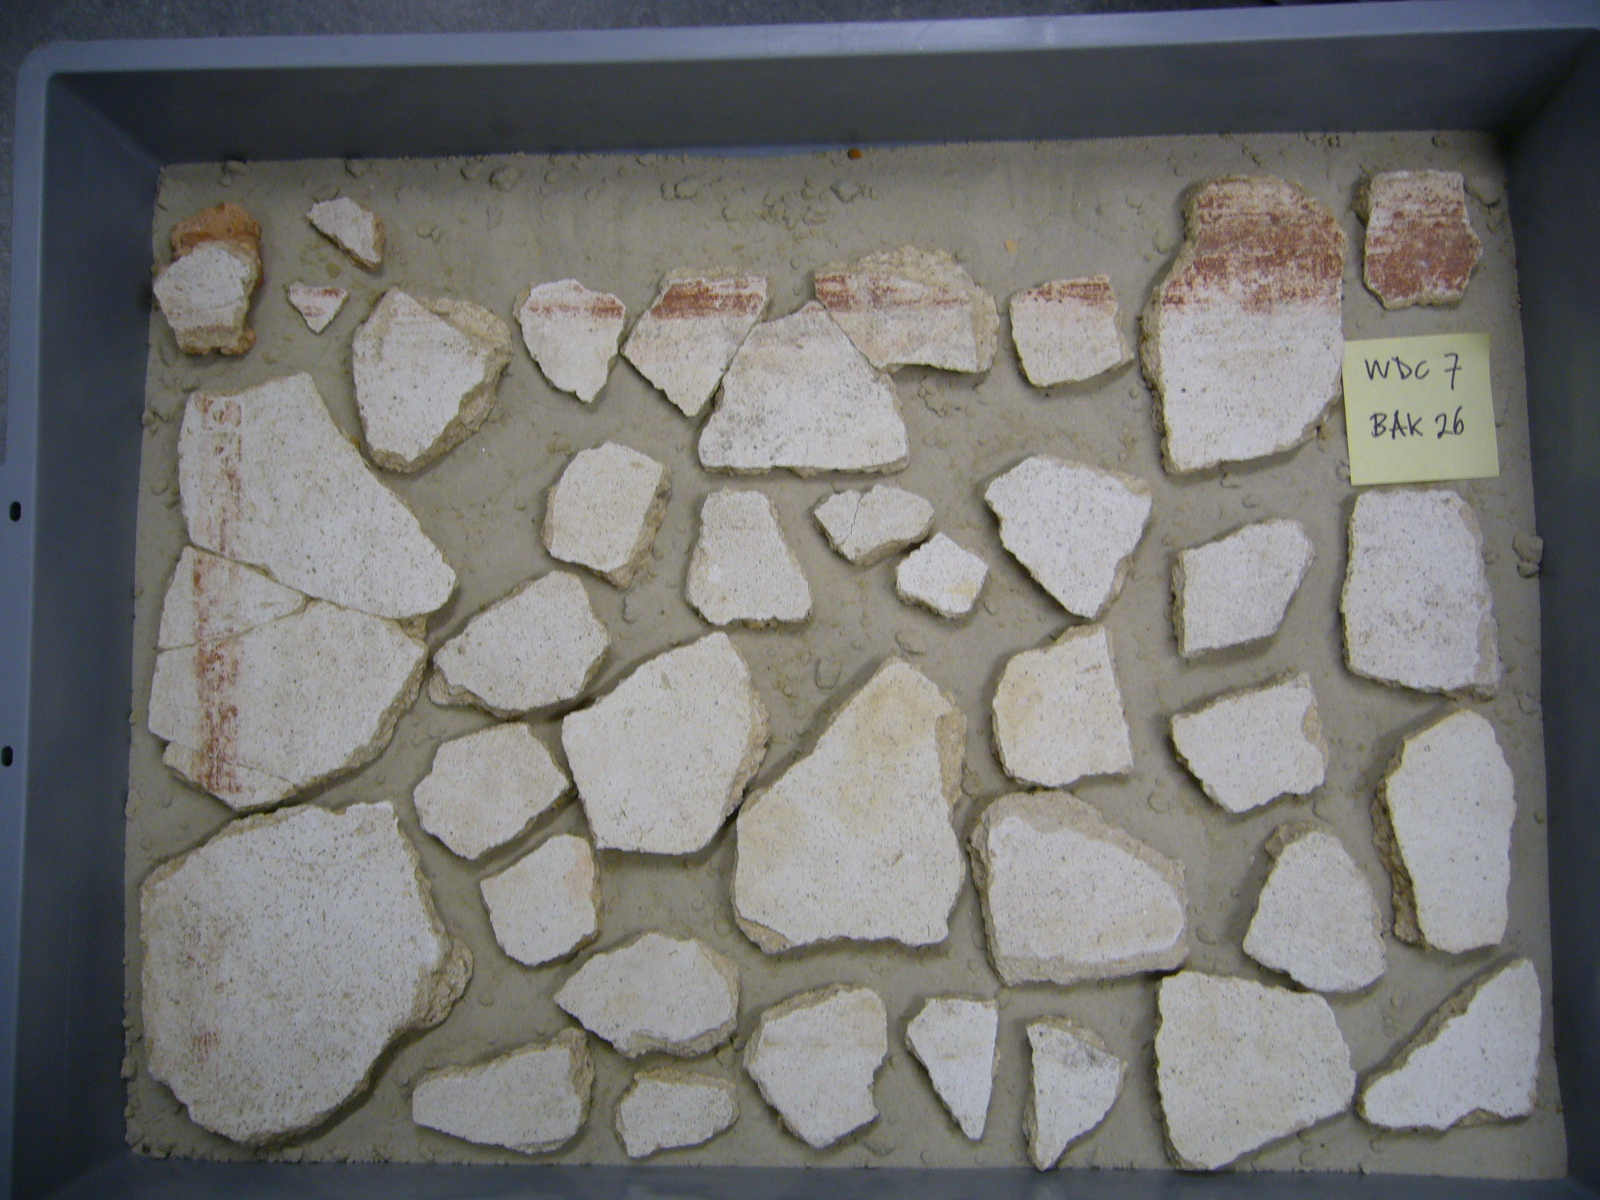
\includegraphics[width=0.6\columnwidth]{images/WDC7_26.JPG}
		\caption{Een bak vol fragmenten die rond dezelfde locatie zijn gevonden, sommige zijn reeds aan elkaar gezet.}
		\label{fig:bakinleiding}
	\end{center}
\end{figure}

De stukken met een nog zichtbaar geometrisch patroon of van de rand van het fresco zijn in vergelijking met de anderen eenvoudig met elkaar te verbinden. Zij zijn door een ervaren archeoloog zonder hulp in elkaar te passen. De overige fragmenten die minder informatie bevatten zijn echter een nachtmerrie om aan elkaar te puzzelen. Er ontbreekt informatie die een structuur vanop een afstand laat zien, het menselijke visuele systeem is blijkbaar niet erg geschikt enkel grillige randen te vergelijken en aan elkaar te zetten. Het enige alternatief lijkt om lokaler te zoeken en elk fragment te vergelijken met elk ander fragment. Deze aanpak is natuurlijk niet mogelijk, er zijn miljoenen combinaties van fragmenten mogelijk.\\

In deze context situeert zich het thera\footnote{Thera is de oude naam voor het huidige griekse eiland genaamd Santorini, waar het project voor het eerst in de praktijk werd toegepast.} project, dat probeert om het werk van de archeoloog gemakkelijker te maken door middel van een software platform~\cite{Brown2008}. De
redenering achter het project is dat een computer de ondankbare taak voorgesteld in de vorige paragraaf kan automatiseren. Dergelijk systeem werd in 2007 aan de \emph{Princeton} universiteit in Amerika geconcipieerd. Sindsdien is er tot op de dag van vandaag door verschillende onderzoekers van over de hele wereld aan gewerkt. De werking van het systeem wordt in het volgende hoofdstuk nader toegelicht.\\

Deze thesis draait rond het maken van een uitbreiding op het platform. De uitbreiding moet de gebruikers van het systeem in staat stellen om de beschikbare data op nieuwe manieren te gebruiken, te visualiseren, aan te passen en te delen met medeonderzoekers. Aangaande terminologie zullen een paar woorden veelvuldig terugkomen: de termen fragment, brokstuk of gewoonweg stuk verwijzen altijd naar een enkel gebroken deel van het originele fresco. De termen fragmentpaar, paar en voorstel zijn gereserveerd voor een aaneenkoppeling van twee fragmenten op een bepaalde plaats. Het valt te benadrukken dat twee fragmenten met elkaar verschillende paren kunnen vormen, indien zij op verschillende punten raken (ook al liggen die punten niet zo ver uit elkeaar). Om deze reden wordt een paar ook vaak een voorstel genoemd, om te benadrukken dat het een mogelijke configuratie is, maar geen zekere. Verder verwijst deze tekst meermaals naar (automatische) herkenners, dit zijn de identificatiealgoritmen die twee fragmenten aan elkaar proberen passen.\\

\section{Overzicht}
Hoofdstuk~\ref{hoofdstuk:overzicht} geeft een overzicht van het bestaande werk en hoofdstuk~\ref{hoofdstuk:doelen} geeft aan op welke vlakken het project zal uitgebreid worden en waarom. Vervolgens behandelt hoofdstuk~\ref{hoofdstuk:ontwerp} het algemene ontwerp van de applicatie. Hoofdstukken~\ref{hoofdstuk:database},~\ref{hoofdstuk:synchronisatie} en~\ref{hoofdstuk:modules} gaan dieper in op enkele specifieke implementaties van het project zoals de database, de synchronisatie en de modules. Tenslotte volgt een besluit in hoofdstuk~\ref{hoofdstuk:besluit}.

\chapter{Overzicht van het thera project}
\label{hoofdstuk:overzicht}
Zoals eerder gezegd bouwt deze thesis verder op een reeds bestaand project. Om ze beter te kunnen situeren in het geheel is het handig om eerst even het thera project bekijken
en dan te zien waar dit project in past.

\section{De opdelingen van het thera project}
Ruwweg gezien kan het reconstrueren van een fresco met behulp van de computer opgedeeld worden in 3~fasen.

\begin{description}
	\item[Acquisitie] Alle gevonden fragmenten worden ingescand met behulp van 3D en 2D-scanapparatuur om zo een virtueel model van elk stuk te bouwen, zie \cite{Brown2008}.  
	\item[Identificatie] Vervolgens worden deze virtuele fragmenten aan een zogenaamde \emph{matcher} gegeven, die voor elk fragmentenpaar gaat kijken of ze mogelijk op elkaar passen. Er zijn verschillende types ontwikkeld, waarvan \'e\'en van de meeste succesvolle de zogenaamde \emph{RibbonMatcher} \cite{Brown2008} bleek te zijn. Deze \emph{matcher} kijkt enkel naar de randen van de fragmenten en kan dus zelfs volledig kleurloze fragmentparen identificeren. Maar het onderzoek gaat verder, in 2010 werd er een nieuw type ontwikkeld dat zijn analyse baseert op een combinatie van verschillende eigenschappen, zoals de sporen die een borstel kan nalaten bij het kleuren van een fresco \cite{TolerFranklin2010}.
	\item[Classificatie \& Reconstructie] De laatste stap bestaat uit het classificeren van wat de vorige stappen produceren (en zodoende het samenstellen van een fresco). Elk voorgesteld paar moet gecontroleerd worden op validiteit. Verschillende statussen kunnen zo toegekend worden aan
	een paar, zoals: \emph{geconfirmeerd}, \emph{misschien}, \emph{nee}, \emph{conflict}, et cetera. De \emph{matcher} produceert namelijk zeer veel mogelijk passende paren, waarvan slechts een klein deel correct zal zijn. De drempel voor het beslissen wat een paar kan zijn en wat niet wordt in de \textbf{identificatie}-stap zo laag ingesteld omdat men wil vermijden dat twee fragmenten die toch passen genegeerd worden (de kost van zogenaamde ``\emph{false negatives}'' wordt hoog ingeschat).
\end{description}

\section{Reconstructie, de bestaande oplossingen}
Het thesisproject besproken in deze tekst tracht de reeds bestaande hulpmiddelen van de reconstructiefase aan te vullen. Hievoor werden reeds programma's ontwikkeld, namelijk \emph{Griphos} en \emph{Browsematches}. Hierop volgt een bondige bespreking van beide programma's, wat ze kunnen en niet kunnen, en eventuele voor- en nadelen. Deze factoren hebben een belangrijke rol gespeelt in de richting van dit thesisproject.

\subsection{Griphos}

Griphos was het eerste programma gericht op het weergeven en beoordelen van de resultaten van de voorgaande stappen. Het werd ontworpen met het doel een centraal zenuwstelsel te zijn voor alle informatie en met deze uiteindelijk een (zo goed mogelijk) gereconstrueerd fresco te maken. Men kan er zowel aparte fragmenten als fragmentparen ge\"identificeerd door een algoritme op een virtueel tafelblad plaatsen en manipuleren. De idee achter een dergelijke voorstelling komt natuurlijk voort uit een rechstreekse vertaling van wat een archeoloog doet op een werkelijk tafelblad naar de computer.\\

\begin{figure}[ht]
	\begin{center}
		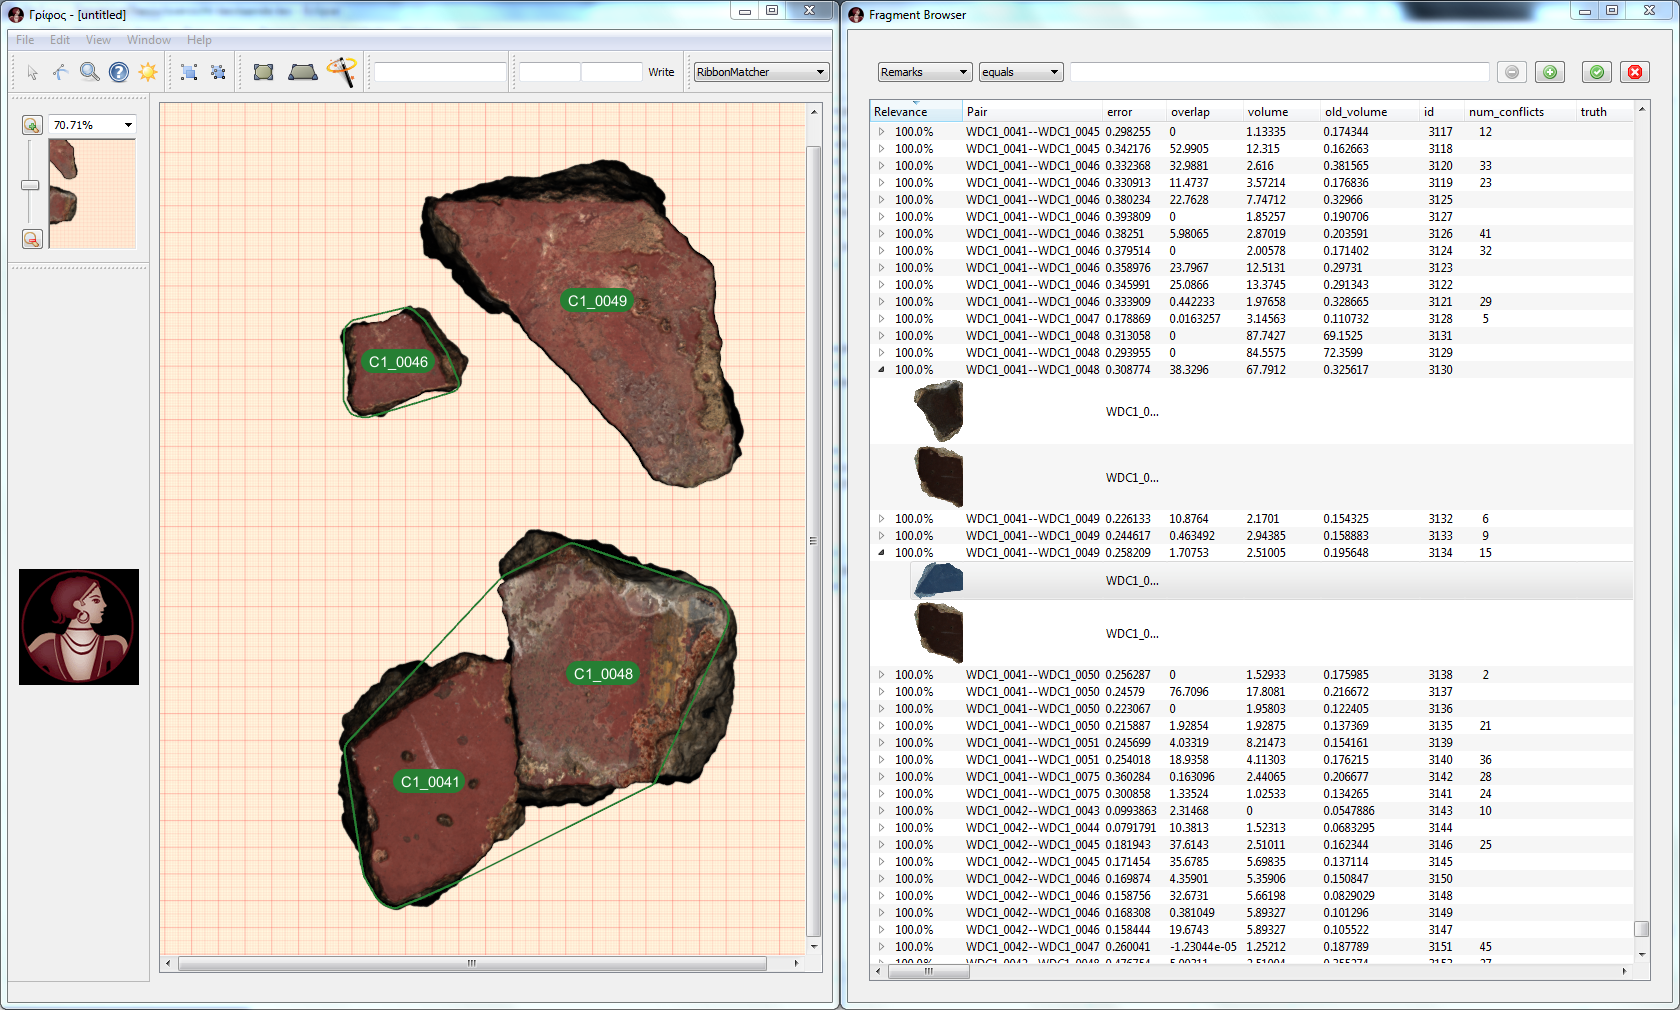
\includegraphics[width=.8\columnwidth]{images/griphos-01-cut.png}
		\caption{Een voorbeeld Griphos tafelblad, 1 voorgesteld paar en 2 aparte fragmenten zijn reeds ingeladen}
	\end{center}
\end{figure}

Het programma wordt echter geplaagd door een paar problemen: het is traag en biedt geen goede wijze aan om de (honderd-)duizenden gegenereerde paarvoorstellen na te kijken. De gebruikte metafoor van het virtuele tafelblad waarin gepuzzeld kan worden stelt weliswaar een belangrijk deel van het reconstructieproces voor, maar schiet tekort als men de nieuwe computergestuurde technieken van fragmentpaar-ontdekking op vloeiende wijze in het proces wil betrekken. Het probleem lijkt te zijn dat er te veel informatie is, en Griphos geen goede manier aanbiedt om door de bomen het bos te zien. De aanzienlijke traagheid van sommige delen van het programma komen vooral voort uit het statische en niet-schaalbare datamodel voor paren (XML bestanden) en de complexiteit van de visualisatie (afbeeldingen van hoge kwaliteit en gedetailleerde 3D-modellen). Dit zorgt voor een soms onaangename werkervaring zelfs indien men er toch in slaagt de juiste fragmentparen te lokaliseren. Desalniettemin is het een krachtig programma dat veel functionaliteit biedt voor de detailinspectie van brokstukken.\\

Het heeft zijn nut al op verschillende vlakken bewezen, behalve detailinspectie is het bijvoorbeeld ook in staat om de posities van fragmenten in een bak te onthouden. Dit betekent een grote snelheidswinst wanneer men bijvoorbeeld denkt een goed paar te hebben gevonden en men wil dit met echte fragmenten verifi\"eren. Als beide fragmenten in dezelfde bak liggen kan het correcte tafelblad ingeladen worden, Griphos kan vervolgens de gezochte fragmenten laten oplichten. Hetgeen veel gemakkelijker is dan zelf te zoeken door de vormen te vergelijken, zeker omdat de brokstukken vaak moeilijk te onderscheiden zijn zoals te zien valt in figuur \ref{fig:griphosbak}. 

\begin{figure}[ht]
	\begin{center}
		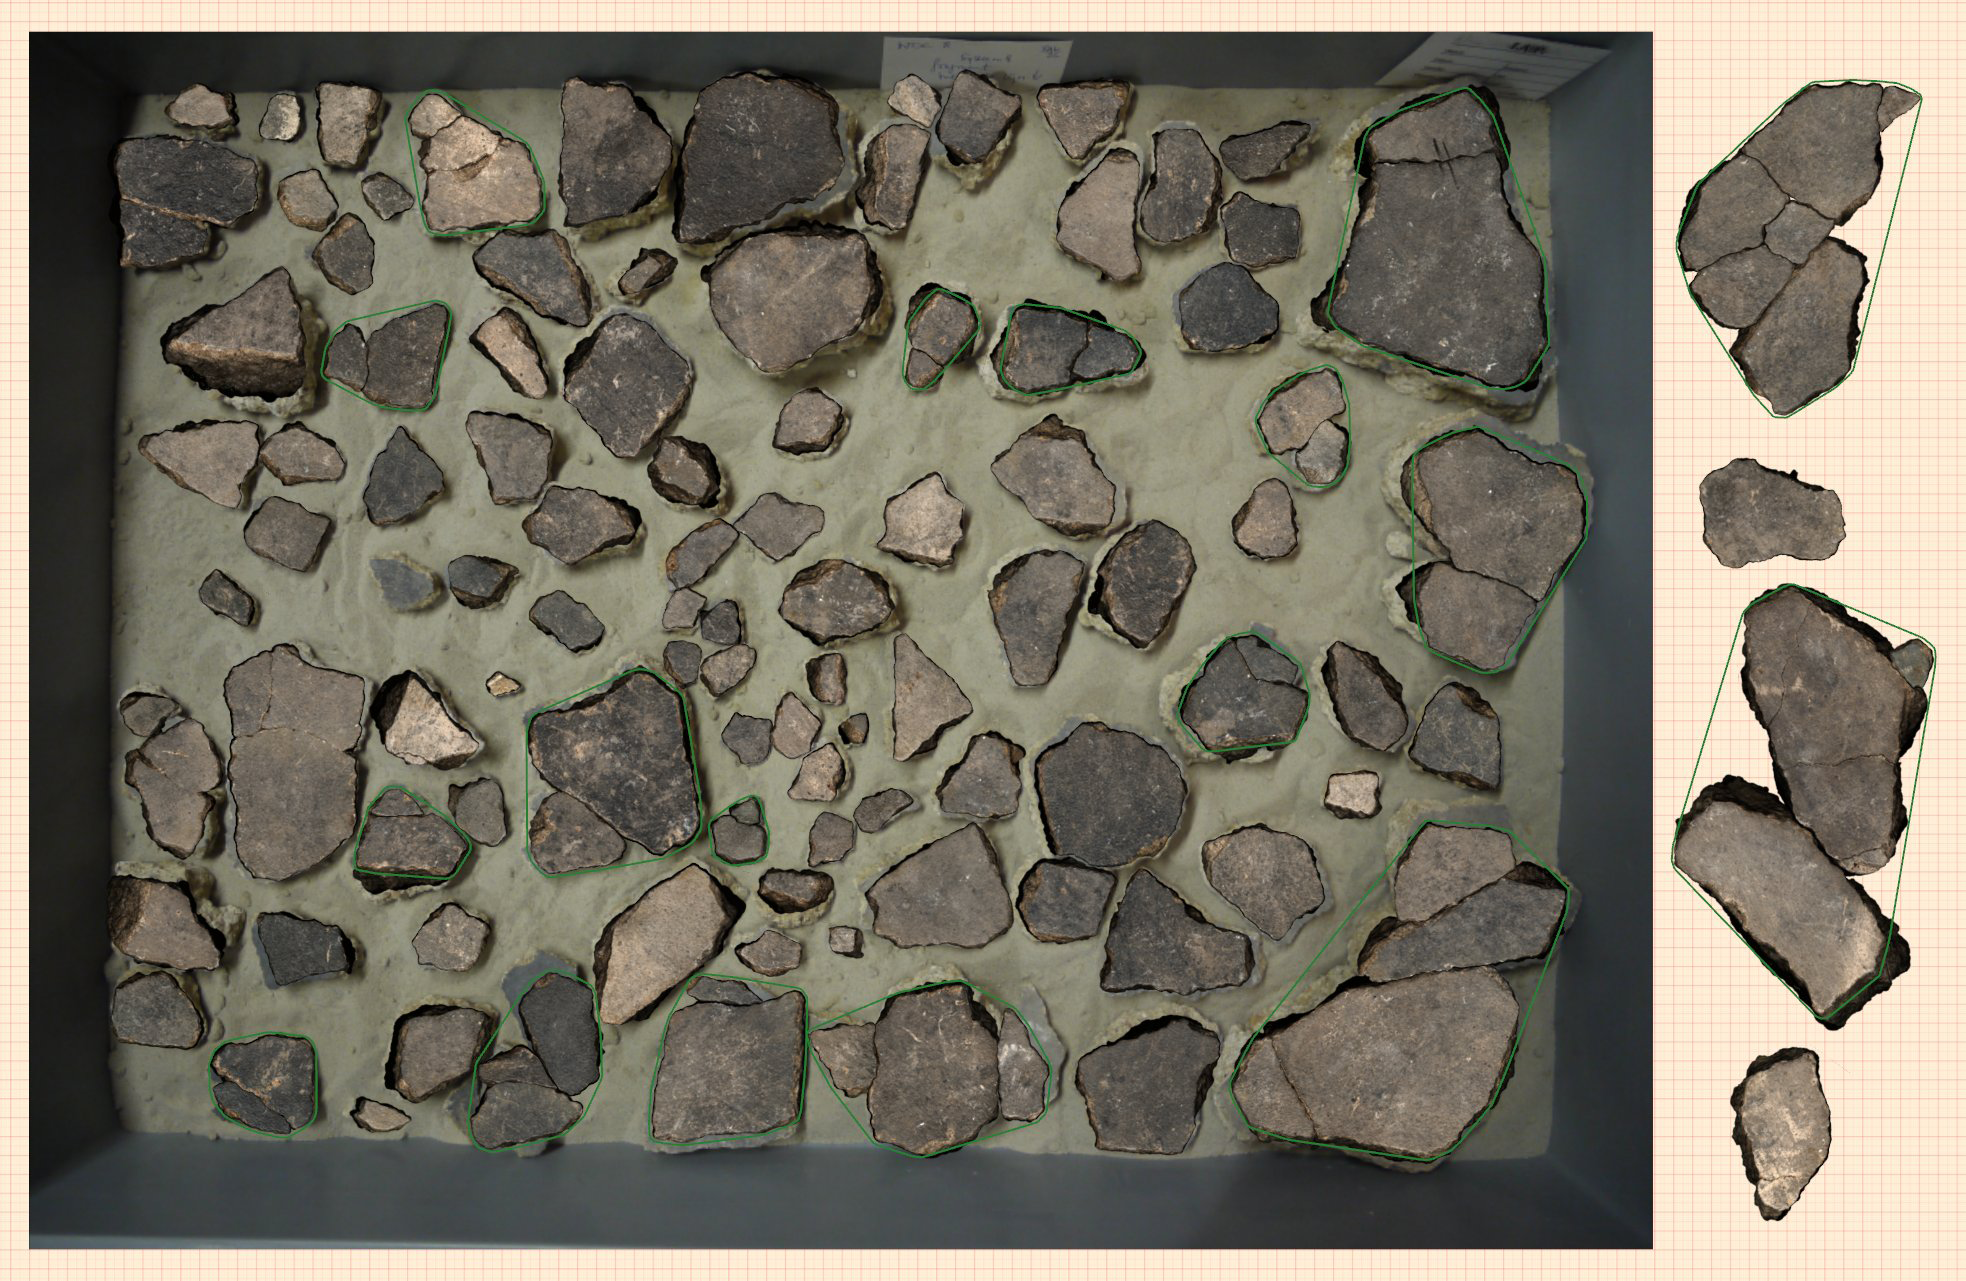
\includegraphics[width=.8\columnwidth]{images/griphos-bak-01.png}
		\caption{Griphos kan gebruikt worden om de posities van fragmenten in hun opslagplaats te onthouden en vervolgens snel terug te vinden. De brokstukken die buiten de bak staan weergegeven zijn verplaatst geweest naar een andere bak. (afbeelding met toestemming gebruikt uit \cite{Brown2011})}
		\label{fig:griphosbak}
	\end{center}
\end{figure}

// te technisch voor dit hoofdstuk, verplaats naar iets later: [TODO: remove]
Het eerste probleem wordt vooral veroorzaakt door trage datatoegang en te complexe visualisaties. Het programma slaagt alles betreffende paren op in een (enorm) XML bestand. Dit is nog doenbaar als men slechts een paar duizend voorstellen heeft maar ondervindt reeds snel onacceptabele vertragingen eens men er meer probeert in te laden. Ter voorbeeld, een kleine voorstellenverzameling van een bepaalde opgraving heeft er reeds 50000. Gekoppeld hieraan laadt Griphos ook steeds een hoge-kwaliteits afbeelding of zelfs een volledig 3D-model in voor elk paar De combinatie van het gebruik van grote XML-bestanden om informatie over de paren in op te slaan, en het steeds inladen van hoge kwaliteits-afbeeldingen en 3D-modellen. om alle info in op te slaan. Dit is bijzonder innefici\"ent en geeft ook bitter weinig mogelijkheden tot uitbreiding. Een ander deel is het gebrek aan zoekmogelijkheden binnen de voorstellen.

\subsection{Browsematches}

Een eerste prototype om de in Griphos ontbrekende delen aan te vullen, werd Browsematches genoemd. Het gebruikte eerst de visualisatiecapabilitieiten van Griphos om kleine afbeeldingen te nemen van elk bestaand paar samen met aan de linkerkant de doorsnede van hun raakvlak, en probeerde er vervolgens zo veel mogelijk te tonen. \\

\begin{figure}[ht]
	\begin{center}
		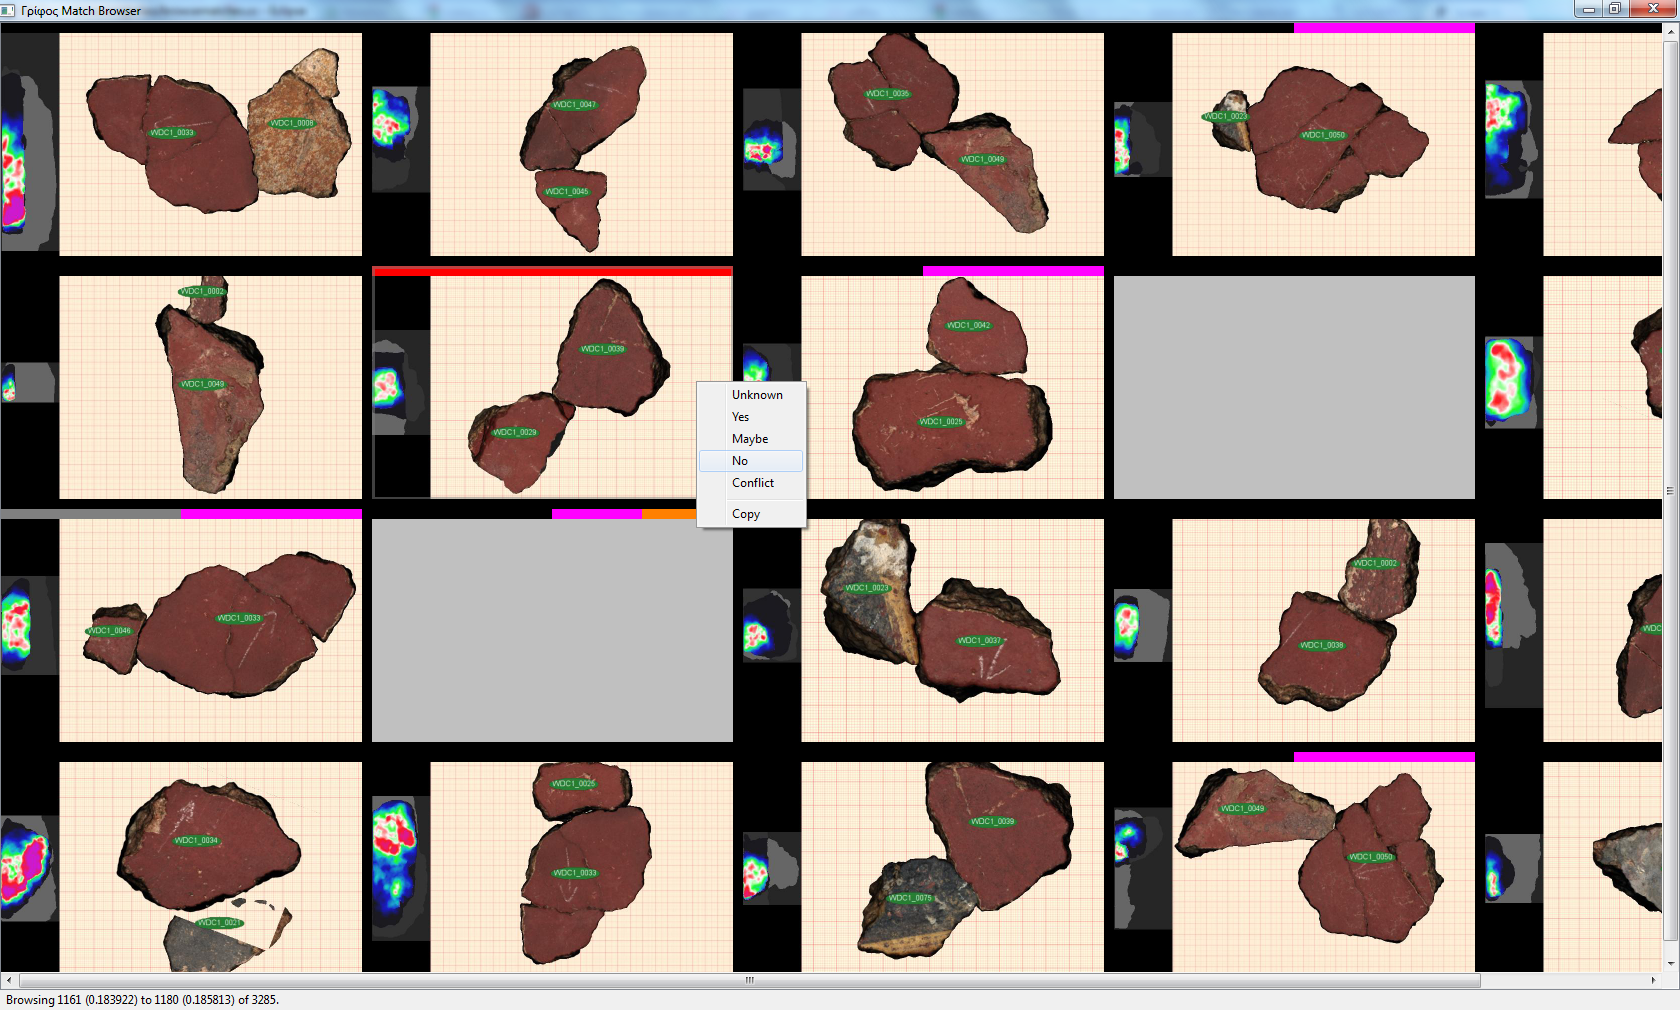
\includegraphics[width=.8\columnwidth]{images/browsematches-01-cut.png}
		\caption{Browsematches in werking, de balken boven de paren duiden een validatie door de gebruiker aan. Rood betekent bijvoorbeeld ``dit voorstel is zeker niet juist''}
	\end{center}
\end{figure}

Dit kleine programma groeide uit noodzaak: het valideren van paarvoorstellen was zo omslachtig met Griphos dat Browsematches in korte tijd in elkaar werd gestoken en met veel succes werd gebruikt om het proces te stroomlijnen. Bij het begin van de thesis, bij wijze van kennismaking met het thera project, werd een verbinding gemaakt met Griphos zodat voorstellen die interessant waren in detail bestudeerd konden worden.\\

Browsematches erfde echter ook enkele van de nadelen van Griphos. [TOOOOOOOOODOOOOOOOOOOOOOO]Het datamodel schaalde nog steeds niet goed, was moeilijk uitbreidbaar en deelbaar en mistte doorzoekbaar, gemakkelijk uitbreidbaar of deelbaar. Daarenboven was het programma slechts een prototype en niet bedoeld voor algemeen gebruik. Het simpele maar succesvolle concept diende als inspiratie en basis voor deze thesis. 

%%% Local Variables: 
%%% mode: latex
%%% TeX-master: "masterproef"
%%% End: 

\chapter{Doelen \& Motivatie}
\label{hoofdstuk:doelen}

Het hoofddoel van het thera project is het reconstrueren van fresco's uit de oudheid zo gemakkelijk mogelijk te maken. Er moet een manier gevonden worden om een waardevolle contributie te maken aan het thera-ecosysteem zodat het zijn doel beter kan vervullen. Dit is onder andere mogelijk door delen die ontbreken aan de vorige oplossingen aan te maken of bestaande componenten veelzijdiger te maken.\\

Gezien de huidige stand van zaken besproken in hoofstuk \ref{hoofdstuk:overzicht}, valt het op dat er nog behoorlijk wat dingen kunnen toegevoegd worden op het gebied van informatie en het visualiseren ervan. De ongelooflijke hoeveelheid data die het thera project reeds heeft geproduceerd en blijft produceren kan op een betere manier behandeld worden zodat het ware potentieel ervan naar de oppervlakte komt. De laatste stap in het sterk geautomatiseerde virtuele reconstructieproces wordt gekenmerkt door een nood aan interactie met de mens die elk soort hulpmiddel moet krijgen om zo correct en snel mogelijke beslissingen te maken. Natuurlijk gaat er niets boven de feitelijke fragmenten fysisch vastnemen en ze aan elkaar te proberen zetten. Maar gezien dit een zeer tijdsrovende bezigheid is, moet dit zo veel mogelijk beperkt worden.\\

Er werd gesproken over Griphos en diens weinig ontwikkelde ondersteuning voor het behandelen van automatisch voorgestelde fragmentparen, alsook over de eerste poging om dit recht te trekken: Browsematches. Deze thesis tracht de lijn van Browsematches verder te zetten, vertrekkende van de goede idee\"en en ervaring waaraan het zijn ontstaan te danken heeft. Dit houdt in dat de focus niet meer zozeer ligt op het actief puzzelen en brokstukken op een tafelblad plaatsen, maar eerder op het beoordelen van de omvangrijke verzameling voorstellen, waarvan slechts een zeer klein deel correct kan zijn. De hoop en verwachting is dat dit zeer kleine deel meteen ook een significante hoeveelheid van de werkelijk overblijvende paren voorstelt.\\

Daarmee valt te benadrukken dat dit project geen vervanging probeert te zijn van de bestaande software, het is eerder bedoeld als een complement. Merk op dat gevalideerde paren niet kunnen conflicteren en dus rechtstreeks in een groep op een tafelblad geplaatst kunnen worden. In de limiet, wanneer alle mogelijke paren correct geclassificeerd zijn vloeit hieruit op natuurlijk wijze een (zo compleet mogelijk) fresco voort. Daarom valt de implementatie in de thesis te zien als een extra tussenstap, chronologisch v\'o\'or het plaatsen van de fragmenten op een tafelblad en na het uitvoeren van de herkenningsalgoritmen. Figuur \ref{fig:flow} stelt dit visueel voor.

\begin{figure}[ht]
	\begin{center}
		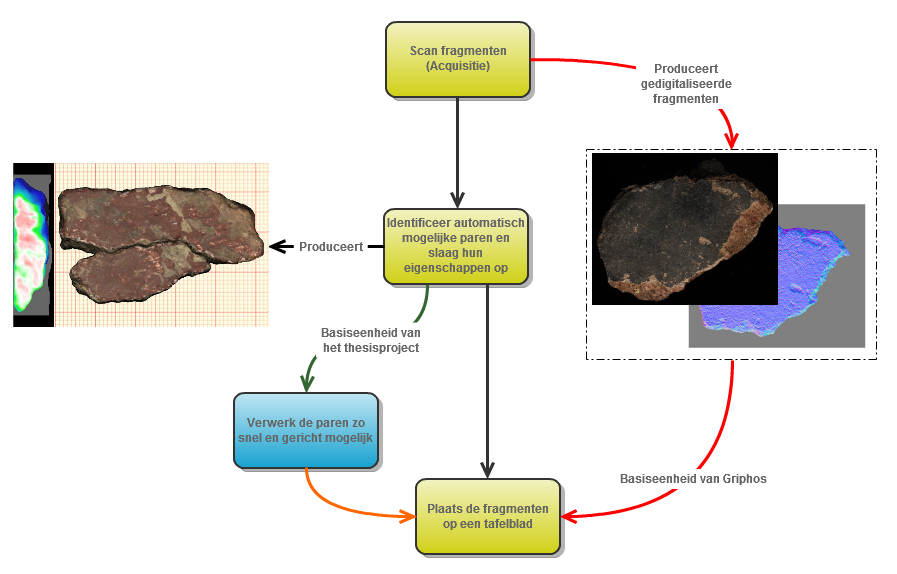
\includegraphics[width=1.0\columnwidth]{images/flowchart-focus-01.png}
		\caption{Het huidige proces met de aanvullingen van de thesis in het blauw}
		\label{fig:flow}
	\end{center}
\end{figure}

Een van de meest fundamentele verschillen tussen de centrale filosofie van Griphos en die van dit project is dus dat terwijl bij Griphos de focus ligt op aparte geplaatste fragmenten, het thesisproject eerder de automatisch gevonden paren behandelt. Het is in Griphos wel degelijk mogelijk om voorstellen van de automatische paarherkenning in te laden maar de naald in de hooiberg vinden is moeilijk.\\

\section{Aspecten waarop de thesis tracht te verbeteren}
Hieronder staan verschillende deelaspecten waarop dit thesisproject verbeteringen tracht te maken. Bij elk aspect staat beschreven wat de vereisten zijn waar het project aan zal moeten voldoen en eventueel een voorbeeldscenario. Men kan deze aspecten desgewenst onafhankelijk bekijken maar vaak steunen ze op elkaar om werkelijk tot hun recht te komen. Een visualisatiemethode heeft bijvoorbeeld een manier nodig om de data die het wil visualiseren te krijgen. Omgekeerd is een databeheersysteem niet bijzonder nuttig zonder de mogelijk de data te manipuleren. Om de verbeteringen en idee\"en te bundelen en te testen is er ook een applicatie gemaakt die dient om reeds een voorproef te geven van wat er mogelijk is met de ontwikkelde technologie.  

\subsection{Integratie}
Zoals eerder vermeld staat dit thesisproject niet alleen maar maakt het deel uit van een groter geheel. Binnen de grenzen van het mogelijke zou er moeten rekening gehouden worden met de integratie van de geschreven code met die van de andere onderzoekers. Dit verhoogt de kans dat het werk aanvaard wordt en ingang vindt in andere subprojecten. 

\subsection{Collaboratie}
Ideaal gezien zouden archeologen steeds toegang moeten krijgen tot hun project op eender welk moment vanop eender welke plaats. Dit kan een gedeelde collectie zijn die over het internet beschikbaar wordt gesteld, of een lokale kopie. Een mogelijk scenario hierbij is dat een ervaren archeoloog in de Verenigde Staten gevraagd wordt om zijn opinie te geven over de huidige stand van zaken (reeds ge\"identificeerde correcte paren, moeilijke gevallen, \ldots). Alle aanpassingen en commentaren die hij maakt worden automatisch ingevoegd en centraal beschikbaar gesteld voor de onderzoekers ter plekke. Op termijn moet het bijvoorbeeld zelfs mogelijk worden om amateurs te laten kijken naar de voorstellen en hun beoordeling te gebruiken om de nog na te kijken voorstellen te rangschikken.\\

Van cruciaal belang is dat alle verzamelde data (zoals de classificatie van voorstellen) op een robuuste manier opgeslagen, gedeeld en ge\"incorporeerd kan worden. De toegang naar en manipulatie van deze informatie moet effici\"ent zijn. De huidige oplossingen zijn hiervoor ontoereikend en traag, zoals besproken in hoofdstuk \ref{hoofdstuk:overzicht}. De mogelijkheid van meerdere en zelfs lokale kopie\"en impliceert ook de nood om te kunnen synchroniseren\footnote{Naar het model van de zogenaamde \emph{Distributed Version Control System (DCVS)} systemen zoals Git, Mercurial, \ldots}. Dit is ook nodig omdat er reeds verschillende huidige verzamelingen bestaan die eventueel in het nieuwe systeem ge\"importeerd en gecombineerd moeten worden. Dergelijk systeem is ook nuttig voor het maken van (kleinere) pocketversies en in gebieden waar de internetconnectiviteit niet adequaat of onbestaande is. Belangrijk is dat er steeds een manier is om waardevolle data te combineren en aan te vullen zodat niets verloren gaat.

\subsection{Schalering}
De bestaande oplossingen voor het valideren van voorgestelde paren werken noodgedwongen met een sterk gereduceerde verzameling. E\'en van de redenen hiervoor is het gebruik van een groot XML bestand om alles in op te slaan. Deze techniek werkt goed voor bijvoorbeeld het opslaan van tafelbladen --- waar er bijvoorbeeld 50 fragmenten en hun locaties moeten opgeslagen worden --- maar schiet tekort voor paarvoorstellen. Een snelle rekensom geeft de reden aan: een laag aantal fragmenten voor een specifieke opgraving is bijvoorbeeld 1500. De meeste paarherkenners gaan alle brokstukken een keer met elk andere brokstuk vergelijken en zodoende het meest waarschijnlijke aankoppelingspunt vinden. Het is zelfs mogelijk dat een fragment meerdere keren een plausibel paar vormt met eenzelfde stuk. Naar onder afgerond komen uit deze stap reeds 2 miljoen configuraties gerold, de ene wat waarschijnlijker dan de andere. Dit nummer stijgt kwadratisch in het aantal fragmenten en zelfs met hogere drempels om volgens een bepaalde maatstaf paren automatisch te verwerpen stijgt het aantal configuraties snel.

\subsection{Gebruiksvriendelijkheid}
De uiteindelijke gebruikers van de applicatie zijn niet de ontwikkelaars van het thera project zelf, maar de archeologen. Om deze reden is het belangrijk dat er rekening gehouden wordt met de noodzaak van een visueel aangename en intuiti\"eve gebruikservaring. Om deze intu\"itiviteit te bereiken moet in het programma steeds de aandacht gevestigd blijven op hetgeen het belangrijkst en meest herkenbaar is: de paren en hun fragmenten. Bij voorkeur moet elke operatie gemakkelijk ontdekbaar zijn in de context waar ze kan gebruikt worden, met eventueel een woordje uitleg erbij.\\

Volgens vele studies op het gebied van gebruikersinterfaces \cite{Hoxmeier00,Shneiderman84,Nielsen94} geraken gebruikers gefrustreerd vanaf een operatie een zekere tijd duurt. Deze frustratiedrempel hangt een af van de aard van de operatie (het resultaat), de frequentie waarmee die uitgevoerd wordt, of er visuele tekenen van voortgang zijn en of er tijdens het wachten (steeds) iets anders kan uitgevoerd worden. Om deze reden is het belangrijk dit aspect in acht te nemen bij het ontwikkelen van de applicatie. Dit is vooral zo omdat veel van de acties die mogelijk moeten zijn het potentieel hebben traag te lopen en dus de gebruiker te frustreren. Een algemene vaststelling: de tijd die een operatie mag innemen is omgekeerd evenredig met de frequentie waarmee deze operatie moet uitgevoerd worden. Deze regel in acht nemend is het duidelijk dat bijvoorbeeld het inladen van een scherm vol voorstellen zoals bij Browsematches, het veranderen van een attribuut van een paar, het filteren en sorteren en dergelijke meer acties zijn die met de grootst mogelijke snelheid moeten worden uitgevoerd. Hoe functioneel ook, een programma dat sloom reageert en elke computer op z'n knie\"en dwingt zal zo weinig mogelijk gebruikt worden \cite{Joel2001}.\\

// hoort mss bij [DESIGN]
De gebruikersinterface van de oude programma's was goed en kon effici\"ent gebruikt worden mits enige training. Maar voor het ondersteunen van collaboratief werken moeten er natuurlijk allerhande nieuwe operaties toegevoegd
worden. Tijdens het implementatieproces werd het duidelijk dat de reeds bestaande code van het Browsematches niet uitbreidbaar genoeg was en die van Griphos te complex en belangrijk. Daardoor werd de beslissing genomen om de
basisinterface van Browsematches over te nemen maar alle onderliggende code te herschrijven zodat die uitbreidbaar zou zijn. Bij het opnieuw construeren van dit alles zijn er een aantal verbeteringen gebeurd die niet meteen te maken hebben met het collaboratie aspect maar wel met de workflow van het classificeren. Dit werd gedaan om het hele programma gebruiksvriendelijker en krachtiger te maken in functie van het hoofddoel van het project.

\subsection{Uitbreidbaarheid}
Het samenstellen van werken uit de oudheid is een zeer vakkennis- en ervaringsintensief proces. Hoewel men luistert naar wat de archeologen hierover te vertellen hebben --- wat ze graag zouden zien of kunnen doen --- zijn er vele zaken die nu nog niet duidelijk zijn maar in de toekomst zeker aan het licht zullen komen. Dit kan bijvoorbeeld zijn omdat de onderzoekers in kwestie niet goed kunnen uitleggen waar ze naar kijken of hoe ze zoeken: na zovele jaren vertrouwen ze op hun moeilijk te defini\"eren intu\"itie. Anderzijds is het vertalen van het proces om fresco's samen te stellen naar de computer nog niet zo vaak geprobeert in het verleden. Dit betekent dat een goede werkwijze in de realiteit misschien niet zonder meer de effici\"entste is als men de transitie naar virtueel reconstrueren maakt (zoals bij Griphos). Daarbovenop zijn er nog vele kansen om innovatieve nieuwe technieken aan te wenden die niet werkbaar zijn als men enkel over fysische fragmenten beschikt.\\

Het is dus onwaarschijnlijk dat het laatste woord over de ideale metafoor reeds gezegd is waardoor er een grote kans is dat het platform zal moeten vervangen of herbouwd worden als het niet met uitbreidbaarheid in gedachte ontworpen wordt. Er moeten moeiteloos nieuwe delen aan de applicatie en de onderliggende lagen kunnen toegevoegd worden om snel nieuwe idee\"en te incorporeren. Dit alles moet best mogelijk zijn zonder de ervaring van gebruikers met oudere versies of andere gebruikersinterfaces te degraderen.

\subsubsection{Data}
De eerder besproken uitbreidbaarheid die nodig is manifesteert zich op het niveau van de data bijvoorbeeld bijboorbeeld op deze manier: een onderzoeker vindt een nieuw algoritme om fragmentparen te rangschikken op ``goedheid'' of men wil informatie over het dikteverschil tussen twee fragmenten opslaan. Idealiter zouden deze zaken als een attribuut bij een paar moeten kunnen toegevoegd worden zodat elke gebruiker er op kan zoeken en sorteren zonder iets extra te hoeven doen.\\
 
Enkel data die op geen enkele manier om te vormen valt naar een attribuut van een enkel paar zal een speciale module vereisen om te kunnen gebruiken. Een vereiste is natuurlijk wel dat dit geen effect mag hebben op de delen van het platform die hier geen weet van hebben.
 
\subsubsection{Visualisatie}
Er zijn vele visualisatiemanieren denkbaar die elkaar kunnen aanvullen bij het volbrengen van het zoek- en classificeerprocess. Zo stelt men zich bij de uitdrukking ``fresco's samenstellen'' waarschijnlijk een grote puzzel voor waar men ten alle tijde het overzicht kan behouden en stukken proberen te passen.\footnote{Het Griphos programma gaat uit van het idee van kleine beheersbare stukken van de reuzenpuzzel (elk tafelblad zou een verzameling kunnen zijn van stukken die gerelateerd waren, bijvoorbeeld door hun vindplaats)} Deze puzzel visualisatie is visueel aantrekkelijk en biedt het menselijke patroonherkenningsvermogen\footnote{Iets waar computers de mens nog altijd niet in evenaren. Een ander thera subproject onderzoekt wel de mogelijkheid om zogenaamde 'clusters' te identificeren en te gebruiken voor reconstructie.} de mogelijkheid om zich van zijn beste kant te laten zien. Echter, door de grote hoeveelheid aan fragmenten en dus mogelijke paren is het moeilijk om hier aan te beginnnen. Maar, hoe meer reeds geconfirmeerde paren er zijn, hoe duidelijker het globale beeld kan worden. Dit staat toe om een overzicht te krijgen van de vooruitgang en gerichter te zoeken naar stukken die nog ontbreken. Dit is een voorbeeld van een macro-perspectief.\\

Een alternatief is te beginnen door te kijken naar waar de computer w\'el goed in is: fragmenten aan elkaar passen en rangschikken naar kans/overeenkomst/et cetera. Door een gemakkelijk navigeerbare lijst op te stellen van alle voorstellen die de reconstructie algoritmes hebben gedaan, kunnen er snel op elkaar passende fragmenten ge\"identificeerd worden. Dit kan men zien als een micro-perspectief of \emph{bottom-up} manier om fresco's te reconstrueren. Het is ook de aanpak die in Browsematches gebruikt wordt. Nadat men bijvoorbeeld met deze manier een deel acceptabele paren heeft ge\'identificeerd, kunnen deze bijvoorbeeld weergegeven worder als een grote puzzel en dienen zij als beginpunt om verder te puzzelen. Dit maakt het globale beeld veel informatiever: stel dat duidelijke "gaten" ontstaan in een resem goede fragmentparen, dan kan er gericht gezocht worden naar een fragment dat erin past door te zoeken naar een fragment dat met elk van deze insluiters past (indien het gevonden werd bij de opgraving).\\

Kortom, het is duidelijk dat een visualisatie die in alle gevallen de meest geschikte is niet bestaat. De beschikbare informatie moet soms gewoon op andere manieren worden weergegeven. Om deze reden is het wenselijk om het mogelijk te maken snel nieuwe visualisaties in te bouwen die kunnen communiceren met andere delen van de applicatie en eventueel de informatie manipuleren. 
\chapter{Ontwerp van het project}
\label{hoofdstuk:ontwerp}

Eenmaal de belangrijkste vereisten gekend zijn kan er een ontwerp opgetekend worden. Daarom even de grote lijnen die te concluderen vallen uit hoofdstuk \ref{hoofdstuk:doelen}:

\begin{itemize}
  \item De data en het visuele aspect van de applicatie moeten zo ontkoppeld mogelijk zijn, elk moet apart uitbreidbaar zijn
  \item Zeer grote hoeveelheden data moeten vlot kunnen behandeld en genavigeerd worden: zoeken, filteren, sorteren, aanpassen, \ldots
  \item De data moet zowel centraal als decentraal toegankelijk zijn en synchronisatie toestaan
  \item Compatibiliteit met de reeds geschreven onderdelen van het project moet indien mogelijk bewaard blijven
  \item Om het ontwerp te verifi\"eren moet een werkend programma gemaakt worden, gebruiksvriendelijkheid, functionaliteit en snelheid zijn hierbij belangrijk
\end{itemize}

\section{De grote lijnen}
Van alle vereisten die rechtstreeks invloed kunnen uitoefenen op de architectuur, is de splitsing van de data en de visualisatie waarschijnlijk de meest fundamentele. Een beproefde aanpak om dit te realizeren is het ontwerppatroon genaamd \emph{Model-View-Controller (MVC)}\footnote{Een algemeen overzicht kan men bijvoorbeeld bekomen op \url{http://en.wikipedia.org/wiki/Model-view-controller}}.\\

Het doel is een ontwerp te maken waarin we een visualisatiemethode kunnen verbinden aan de juiste databron. Enkele zaken moeten echter nog vastgelegd worden, namelijk: wat is de basiseenheid van data? Waar zal een visualisatiemodule achter vragen? Zoals in figuur~\ref{fig:flow} te zien is, ligt de focus bij dit project op koppelingen van fragmenten in plaats van fragmenten op zich. Er zijn op het eerste zicht twee alternatieven om dit te modelleren. De eerste mogelijkheid is een soort van \emph{MatchedFragment} die een fragment beschrijft plus een lijst met alle fragmenten die er potentieel aan gekoppeld kunnen worden en op welke locatie. De tweede mogelijkheid is om elk paar een apart object te laten voorstellen (bvb. genaamd \emph{FragmentPair}). Het eerste alternatief lijkt het voordeel te hebben dat het gemakkelijk is om na te kijken of een fragment reeds ``bezet'' is. Ook zou het dan mogelijk zijn om bijvoorbeeld een grafe op te stellen door van brokstuk naar brokstuk te springen. Echter, dit soort opstelling bevat op het eerste zicht veel redundantie, een fragment zal op die manier een verwijzing met attributen naar een fragment bevatten, en dit fragment zal op zijn beurt een identieke omgekeerde verbinding hebben. De redundantie vermijden en een verwijzing als een apart object voorstellen waar beide fragmenten naar kunnen verwijzen is eigenlijk niets anders dan de tweede optie (een \emph{FragmentPair}). Op die manier wordt de situatie omgedraaid en kan een fragmentenpaar verwijzen naar de fragmenten die het opbouwen. Daarbij kan het probleem van hoe de ``bezetting'' van een object te weten te komen (alsook de grafe, zoals later zal aangetoond worden) opgelost worden door de vereiste zoekfunctionaliteit van het datamodel te benutten.\\

Eenmaal de basiseenheid van informatie gekozen is, valt de kern van de applicatie volgens MVC uit te beelden als in figuur~\ref{fig:basicprogramflow}.

\begin{figure}[ht]
	\begin{center}
		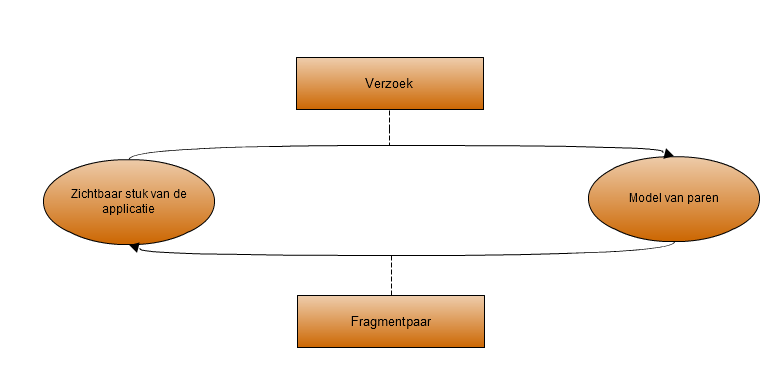
\includegraphics[width=1.0\columnwidth]{images/BasicExecutionFlow.png}
		\caption{Het abstracte model van de applicatie, links staat de \emph{View/Controller} en rechts het \emph{Model}. De controller stuurt een verzoek naar het model voor een bepaalde (sub)set van de data --- al dan niet gesorteerd --- en het model antwoord met alle paren die voldoen aan de criteria}
		\label{fig:basicprogramflow}
	\end{center}
\end{figure}

\subsection{Modellen}

\ldots Elk model heeft een selectie die ook gedeeld kan worden

\subsection{Verzoeken}

\subsubsection{Opvragen}
Het concept achter het opvragen van fragmentparen is dat er steeds wordt begonnen vanuit de volledige beschikbare verzameling. Deze kan dan \textbf{gereduceerd} en \textbf{gesorteerd} worden. \\

Sorteren is eenvoudig en kan op eender welk attribuut in stijgende of dalende zin gebeuren. Filters gebruiken een simpele maar krachtige syntax die volledig gelijk is aan die van de \emph{WHERE}-clausule van een SQL zin (voorbeeld: broncode~\ref{code:sortingfiltering}). Geavanceerde gebruikers kunnen op deze manier zelf filters verzinnen, veelgebruikte filters en sorteeroperaties kunnen echter best als knoppen en invoervelden blootgesteld worden, zoals in figuur~\ref{fig:tangfiltersort}.\\

De voorwaarde die aan filters gesteld wordt is dat ze enkel attributen beschrijven die werkelijk bestaan, filters die naar een onbestaand attibuut refereren worden genegeerd.\\

Er kunnen meerdere filters op een model actief zijn, deze werken dan conjunctief. Op die manier kunnen meerdere modellen filters plaatsen zonder met elkaar in conflict te komen. 

\lstinputlisting[language=C++,label=code:sortingfiltering,caption=Een voorbeeld van hoe een model kan gebruikt worden in een applicatie]{source/sortingfiltering.cpp}

\begin{figure}[ht]
  \centering
  \subfloat[Sorteren]{
    \label{fig:tangsorting}
    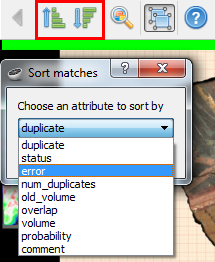
\includegraphics[width=0.30\textwidth]{images/tangerine-sorting.png}
  }\hfill%%%%%%%%%%%%%%%%%%%%%% <========
  \subfloat[Filteren op namen van fragmenten]{
    \label{fig:tangfiltering}
    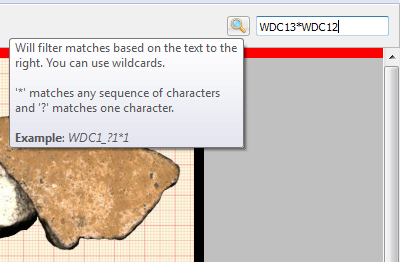
\includegraphics[width=0.60\textwidth]{images/tangerine-namefilter.png}
  }
  \caption{Basis sorteer- en filteroperaties worden via de gebruikersinterface blootgesteld}
  \label{fig:tangfiltersort}
\end{figure}

% \begin{figure}[ht]
%   \begin{minipage}{0.30\textwidth}
%     \centering
%     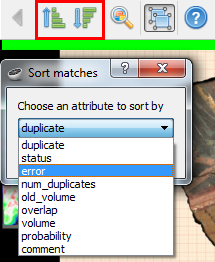
\includegraphics[width=0.60\textwidth]{images/tangerine-sorting.png}
% 	\caption{Sorteren}
% 	\label{fig:tangsorting}
%   \end{minipage}\hfill
%   \begin{minipage}{0.60\textwidth}
%     \centering
%     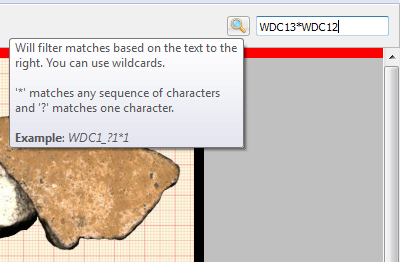
\includegraphics[width=0.60\textwidth]{images/tangerine-namefilter.png}
% 	\caption{Filteren op de namen van de fragmenten}
% 	\label{fig:tangfiltering}
%   \end{minipage}\hfill
% \end{figure}

\subsubsection{Aanpassingen}
Veranderingen aan de inhoud van de database 
Een verzoek\ldots

Er zijn twee grote klassen
Er kan gesorteerd worden op attributen en er kan gefilterd worden o

\subsection{Fragmentenparen}
Het zoeken naar de gewenste verzameling van paren gebeurt via een verzoek en wordt aan het model overgelaten, maar wat kan een component doen met de paren die dan ter beschikking komen? Op zijn minst bestaat een paar uit twee fragmenten en een resem eigenschappen. Die eigenschappen of attributen kunnen gaan van een maatstaf voor de fout toegekend door de automatische herkenner, tot de validatie die een onderzoeker aan het voorstel heeft gegeven. De objecten die geproduceerd worden door de automatische paarherkenners van het theraproject voldoen aan deze twee voorwaarden. Er bestaan reeds veel componenten die hiervan gebruik maken dus dezelfde interface recycleren zou de integratie van het project een heel deel vergemakkelijken. Alle aanpassingen die zich niet kunnen beperken tot \'e\'en paar kunnen via het model afgehandeld worden.\\

\section{Modulariteit}
Om het geheel uitbreidbaar te maken is een pluginsysteem gemaakt. Er is een hoofdapplicatie (codenaam ``Tangerine'') die de connectie maakt met de databeheerlaag en verschillende visualisatieplugins kan laden. Het basissysteem zonder modules bestaat uit een manier om een fragmenten en paren-database in te laden en te kiezen welke module op te starten.\\

De eerste en meest uitgewerkte daarvan werd \emph{MatchTileView} gedoopt. Het geeft de paren op dezelfde manier weer als het Browsematches prototype, maar is natuurlijk uitgebreid qua mogelijkheiden. De bespreking van de toegevoegde functionaliteiten komt aan het bod in het hoofdstuk over modules.\\

\begin{figure}[ht]
	\begin{center}
		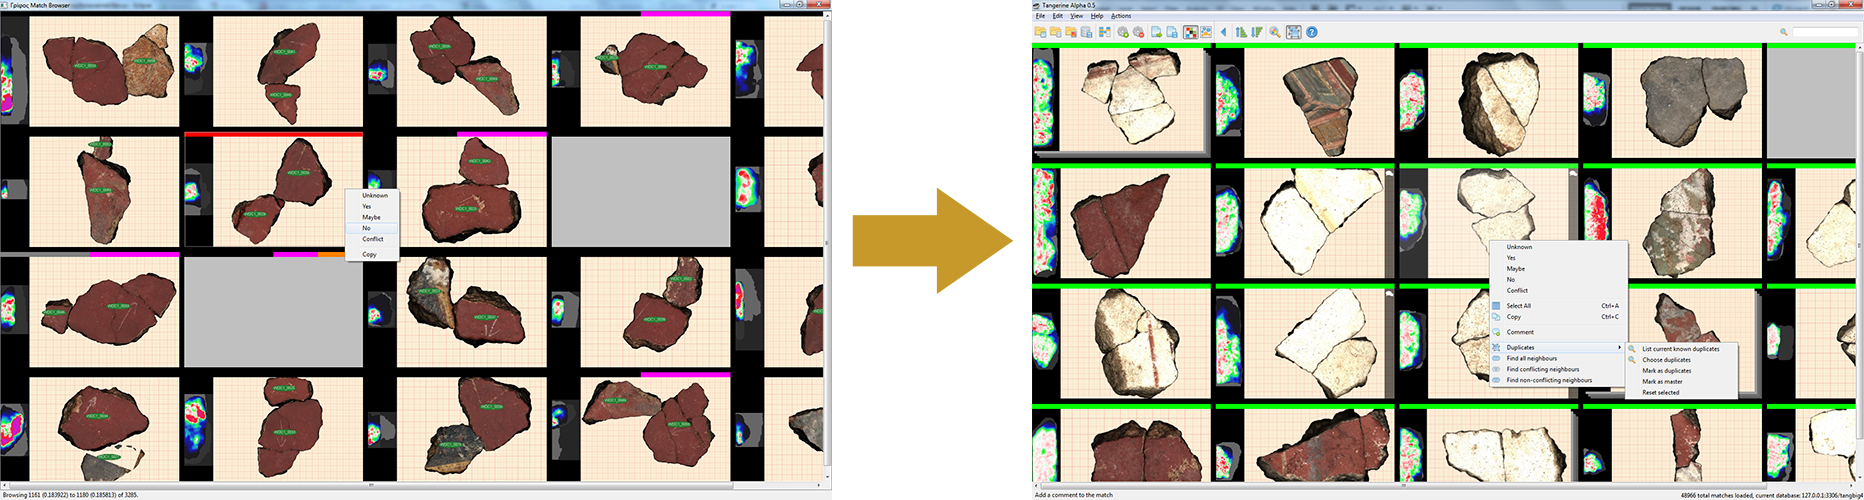
\includegraphics[width=1.0\columnwidth]{images/browsematches-to-tangerine-01.png}
		\caption{De manier van weergeven uit Browsematches werd gekopi\"eerd naar het nieuwe platform, met uitbreidingen}
		\label{fig:browsematchestotang}
	\end{center}
\end{figure}

Elke module krijgt van de applicatie een model toegewezen waar het fragmentparen uit kan opvragen. Dit kan een nieuw model zijn zonder criteria of een gedeeld model. Een gedeeld model behoort niet exclusief tot een module en betekent bijvoorbeeld dat als er \'e\'en beslist om te sorteren op een attribuut zoals ``het verschil van de dikte tussen twee fragmenten'', alle modules die gebruikmaken van ditzelfde model opeens over een gesorteerde dataset beschikken. Via speciale signalen worden zij hiervan op de hoogte gebracht, zodat ze kunnen beslissen of het nodig is een actie te ondernemen. Dit kan handig zijn voor pure visualisatieplugins die geen zoekmogelijkheden aan de gebruiker blootstellen, het kan dan vertrouwen op andere modules om data aan te leveren.\\

Indirecte communicatie via het model is (voorlopig) de enige manier waarop modules elkaar kunnen be\"invloeden. De structuur van de componenten ziet er uit als in figuur~\ref{fig:visualizationlayer}. Merk op dat er een plugin is (\emph{DetailView}) die geen gebruik maakt van fragmentparen maar eerder van een virtueel tafelblad net als Griphos. Zoals eerder aangehaald kunnen fragmentparen automatisch op een tafelblad gezet worden. Dit tafelblad kan dan in 3D weergegeven worden door \emph{DetailView}, waarover later meer.

\begin{figure}[h]
	\begin{center}
		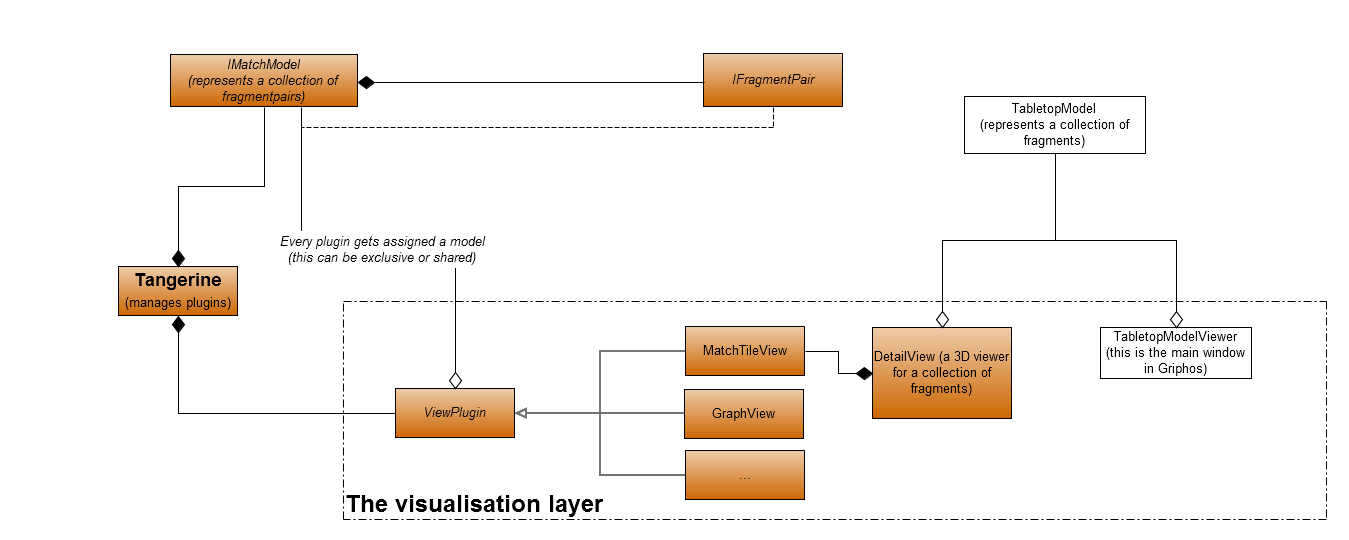
\includegraphics[width=1.0\columnwidth]{images/VisualizationExtract.png}
		\caption{Een vereenvoudigde kijk op de componenten van de visualisatielaag, het hoofdscherm en het model. De componenten in het wit behoren tot de rest van het thera project en zijn niet gemaakt als deel van dit thesisproject.}
		\label{fig:visualizationlayer}
	\end{center}
\end{figure}

\section{Dataoplsag, synchronizatie, \ldots}
De oplossing om aan de vereisten van centrale en decentrale toegang, grote hoeveelheden data en navigatie te voldoen wordt in hoodstuk \ref{hoofdstuk:database} besproken. Het is echter reeds duidelijk dat er een database zal moeten gebruikt worden. Om twee van deze databases te verenigen is er een component ontwikkeld die een aantal fasen doorloopt. De mogelijkheid bestaat om er later nog meer te maken maar voorlopig zijn er 3 fasen: \textbf{Gebruikers}, \textbf{Paren} en \textbf{Attributen}. In elke fase krijgt de gebruiker een scherm te zien met de verschillen tussen de 2 databases die een algoritme heeft gedetecteerd en krijgt ze de mogelijkheid om aanpassingen te maken alvorens naar de volgende fase over te stappen. Het is belangrijk gebruikers keuzes te laten maken waarin ze ge\"interesseerd zijn en ze niet lastig te vallen met keuzes die ze niet willen maken (beide zaken negeren leidt tot frustraties~\cite{Joel2001}). Het algoritme probeert steeds een standaardkeuze in te vullen aan de hand van heuristieken (dit hangt af van de fase), de gebruiker kan deze indien gewenst natuurlijk veranderen. Tegelijkertijd moet de gebruiker ge\"informeerd worden van alle stappen die het algoritme zal ondernemen. 

\subsection{Paren}

Overeenkomsten met verschillende id
Overeenkomsten met dezelfde id
Conflicten met dezelfde id
Geen conflict, geen overeenkomst

Deze subcomponent laat aan de volgende fasen weten welke acties er zijn ondernomen, meer bepaald welke id-transformatie een bepaalde object heeft meegemaakt

\subsection{Attributen}
\subsection{Geschiedenis}

\section{Gebruiksgemak / visuele interface}
De gebruikersinterface en de achterliggende bibliotheken werden gemaakt met behulp van de Qt toolkit~\cite{qtdoc}

Vergelijking van wachttijden tussen Griphos/Browsematches en Tangerine

Geheugengebruik BM na grote db: 350 MB (geen afbeeldingen)

Griphos: tonen van een lijst met aparte fragmenten om uit te kiezen (geen equivalent in BM/Tang)
Griphos: tonen van een lijst met alle paren (zoals te zien in figuur~\ldots): 7 minuten 18 seconden <--- NOOT: Griphos gebruikt dezelfde manier van fragmenten inladen als Browsematches, maar laadt ook op voorhand alle afbeeldingen in. Het geheugengebruik na het openenen van 49471 paren is 1.5 GB RAM, het heropenen van dit scherm neemt evenveel tijd in beslag. Het lijkt erop dat het geheugen niet vrijgemaakt noch herbruikt wordt, want bij de tweede keer moest het besturingssysteem het programma afsluiten wegens te veel geheugengebruik.
Browsematches: opstarten en een lijst van alle paren tonen: 49471 paren = 160 seconden en 350MB
Thesisproject: 

\rowcolors{2}{gray!50}{white}
\begin{center}
	\begin{tabular}{|l|r|r|r|}
	    \rowcolor{gray!75}
	    \hline
	    & \textbf{Griphos} &  \textbf{Browsematches} & \textbf{Thesis (MySQL)} \\
	    \hline
	    \textbf{Opstartsnelheid} & 1 sec & 16 sec & 1 sec \\
	    \textbf{Fragmenten inladen} & 1 min 35 sec  & - & - \\
	    \textbf{\textasciitilde 4000 paren laden} & - & 16 sec & 0 sec \\
	    \textbf{\textasciitilde 50000 paren laden} & 7 min 18 sec & 2 min 47 sec  & 0-3 sec* \\
	    \textbf{\textasciitilde 250000 paren laden} & niet getest & niet getest & 0-15 sec* \\
	    \hline
	\end{tabular}
\end{center}

* Deze getallen zijn afhankelijk van de cache die op de moment aanwezig is, enige vorm van recente activiteit op de database zal ervoor zorgen dat de responstijd rond de 100 milliseconden ligt. De reden dat het soms lang duurt is omdat het programma vraagt achter het totaal aantal fragmenten, en dit is voor de geteste types van databases geen snelle operatie (alles moet geteld worden). Het cijfer verchilt ook per type database

Alle informatie die alleenstaande brokstukken toebehoort --- naam, 3D-voorstelling, contour, \ldots --- wordt opgeslagen als een grote verzameling mappen in het bestandssysteem. Hoewel niet alles meteen wordt ingeladen neemt dit soms toch wat tijd in beslag. Hetzelfde geldt voor een collectie paarvoorstellen waarvan een eerste scherm moet ingeladen worden. Weer een andere bron van vertraging bij het opstarten is het inladen van alle modules, vooral degene die gebruikmaken van OpenGL om fragmenten in 3D weer te geven. Deze stappen  Om deze reden is er voor gezorgd dat deze operaties parallel kunnen lopen, zodat de gebruiker zo weinig mogelijk moet wachten en steeds informatie kan krijgen over de vooruitgang.

De gemiddelde opstarttijd voor Browsematches gemeten op een AMD Athlon X2 5600+ met 2 GB RAM is 10 seconden, waardoor de gebruiker reeds snel gaat denken dat er iets misgelopen is. Bij Browsematches duurde het bijvoorbeeld  is nog  een. 

Alle modules kunnen acties zoals knoppen en menu's  Elk programma dat Bij het initialiseren 

% DATA
\section{Het beheer van de data}

Redenering: Alles vloeit voort uit de paren, het is voorspelbaar (simpel voor te stellen) en ondubbelzinnig

Het zelf kunnen maken van paren is van secundair belang (volgens de thesis), zij kunnen door de HumanMatcher ingevoerd worden in de grote database

Griphos is zeer nuttig -> identificatie locatie van fragmenten in de bak, etc. -> Tangerine is het ontbrekende middendeel!

Dit betekent echter niet dat beide perspectieven elkaar uitsluiten, integendeeel.
 
[TODO: verhuizen naar ontwerp van database]

% VISUALISATIE
\section{Visualisatie, een manier om met de data te werken}

\subsection{Model-View-Controller}

\subsection{UML diagramma}

[maak UML diagramma]\\

\section{Integratie in thera project}
Gebruik van bibliotheken, ...
Extensie door refactoring: FragmentConf -> IFragmentConf ==> SQLFragmentConf | FragmentConf
Hierdoor is het nodig om de reeds bestaande code van het thera project om te zetten naar het gebruik van IFragmentConf waar mogelijk maar het aanmaken van FragmentConf anderzijds
of FragmentConf ==> SQLFragmentConf
Alternatieve oplossing, geen veranderingen in thera code maar SQLFragmentConf sleept dan veel onnodige ballast mee van FragmentConf

\section{Uitbreidbaarheid}
[afbeeldingen invoegen]\\


[afbeelding invoegen, selectie naar grafe transit!]\\
\chapter{Bespreking van het database ontwerp}
\label{hoofdstuk:database}
De visuele delen van het platform bekommeren zich met de \textbf{de manier waarop} er data moet weergegeven worden, de gebruiker kiest \textbf{wat} er moet weergegeven worden. Om de data hiervoor aan te voeren is er een datalaag nodig die elk verzoek juist en effici\"ent kan verzorgen.\\

De hoofdpunten waaraan deze laag moet voldoen werden reeds opgesomd in hoofdstuk~\ref{hoofdstuk:doelen}, namelijk: snelheid, universele toegang, synchroniseerbaarheid en maximale flexibiliteit voor data-analyse. Eerst wordt een analyse gemaakt van de structuur van de data. Vervolgens wordt er gekeken naar de huidige methode die het thera project hiervoor hanteert. Enkele alternatieven worden besproken en op basis daarvan wordt een keuze gemaakt.\\

Alle tijdmetingen werden opgenomen met hetzelfde systeem, een AMD X2 5600 (dual core) met 2GB RAM en een 7200 RPM harde schijf. Als besturingssysteem werd Windows 7 64-bit gebruikt.

\section{Ontleding van de data}

\subsection{Aanwezige data}
De kern van de data is een verzameling fragmentparen, deze bezitten elk een paar onmisbare eigenschappen en vele optionele attributen. De basiseigenschappen beperken zich tot de namen (of een identificatienummer) van de fragmenten en een transformatiematrix die het \'ene brokstuk aan het andere koppelt in de ruimte. Er is geen enkel paar dat deze gegevens mist. Verder kunnen de herkenningsalgoritmen en eventuele \emph{post-processing}-algoritmen allerlei soorten data toevoegen als attributen. Dit kan gaan om een maatstaf afhankelijk van het pasproces zoals de zogenaamde \emph{RibbonMatcherError}~\cite{Brown2008} of een algemene eigenschap zoals het het overlappende volume van twee brokstukken. Verder kan een gebruiker eigen data toevoegen, zoals een validatie, commentaar bij een voorstel, et cetera.

\subsection{Extra data}
De data uit het vorige stuk is reeds terug te vinden in het thera project, maar om collaboratie toe te laten moeten een paar zaken zoals gebruikers en geschiedenis toegevoegd worden.

\subsubsection{Gebruikers}
Behalve paren en attributen is het in een collaboratieve omgeving handig om gebruikers bij te houden. Omdat het systeem in eerste instantie voor selecte groepen is, is een gebruikersnaam en een mailadres voldoende. Op die manier zou men kunnen vastleggen wie welk stukje data heeft toegevoegd of veranderd. Dit is nuttig om de oorzaak van problemen op te sporen als die zich voordoen en te beslissen wiens data voorrang krijgt als eenzelfde fragment door een andere persoon gewijzigd wordt (zie synchronisatie).

\subsubsection{Geschiedenis}
Synchronisatie is een vereiste, hetgeen detectie en resolutie van conflicten impliceert. Om de resolutie voor een deel te automatiseren is een geschiedenis van de attributen nodig (zie hoofdstuk~\ref{hoofdstuk:synchronisatie}). Dit wil zeggen een lijst die aanduidt op welk moment, door wie en naar welke waarde een attribuut is veranderd. Het bijhouden van een geschiedenis heeft ook andere voordelen, zo kan bijvoorbeeld de geschiedenis van een ``commentaar''-attribuut gebruikt worden als een manier om te corresponderen. De overgang van validaties van een paar (bijvoorbeeld \emph{niet geweten} $\rightarrow$ \emph{misschien} $\rightarrow$ \emph{niet correct} of  \emph{niet geweten} $\rightarrow$ \emph{misschien} $\rightarrow$ \emph{correct}) kan een nuttige bron van data zijn voor zowel mensen (statistieken) als computers (lerende algoritmen).
  
%...relationeel van aard? (de geschiedenis wel, denormalisatie nodig voor NoSQL) => SQL database
%Het Eigenschap-patroon (Property pattern)
%Huidige situatie = Properties pattern? % ( http://steve-yegge.blogspot.com/2008/10/universal-design-pattern.html#redacted )

\section{Het oude systeem: XML-bestanden}
De fragmentparen en hun attributen worden door automatische herkenners opgeslagen in een XML bestand zoals in lijst~\ref{code:fragxml}. Dit formaat is uitermate geschikt voor het overbrengen van de data naar andere subsystemen en is leesbaar door een mens. Het is minder geschikt als een permanent opslag- en zoekformaat. Griphos en Browsematches gebruiken het XML-formaat ook voor dat laatste, met enkele nadelen tot gevolg. Om een redelijke snelheid te behouden tijdens het zoeken of sorteren moeten ze het bestand volledig in het werkgegheugen plaatsen. Voor een document met 50000 paren neemt dit reeds een goede 300MB in beslag voor paren met elk 11 attributen (zonder afbeeldingen of 3D-modellen). Dit extrapoleren naar een miljoen paren geeft 5GB aan vereist werkgeheugen, hetgeen bij de meeste systemen van vandaag leidt tot het wegschrijven van data naar het bestandsssyteem of eerder nog een geheugenallocatiefout.\\

\lstinputlisting[float=h,label=code:fragxml,caption=Uittreksel van een fragmentpaarbestand (hier worden slechts 2 paren getoond)]{source/shortmatches.xml}

Het inladen van dit XML bestand is tijdrovend. Tabel~\ref{table:matchesloadspeed} laat zien dat dit minutenlang kan duren en geeft een vooruitkijk op de performantie die het thesisproject haalt. Griphos en Browsematches gebruiken dezelfde manier om data in te lezen, maar vertonen evenwel een groot verschil in laadtijd. De reden is dat Griphos meteen ook de afbeeldingen van elk fragment ophaalt. Meer nog, na het laden van 50000 paren neemt het Griphos proces 1.5GB RAM in beslag. Het lijkt erop dat dit geheugen niet onmiddellijk vrijgemaakt noch herbruikt wordt, want een tweede keer de lijst met fragmentparen openen zorgde er op het testsysteem met 2GB RAM voor dat Griphos keer op keer werd afgesloten wegens overallocatie. Browsematches (en de thesisapplicatie) laden de afbeeldingen pas wanneer ze eigenlijk nodig zijn en besparen op die manier veel geheugen. Het thesisproject gaat eigenlijk nog een stapje verder en laadt zelfs de fragmenten pas in wanneer ze nodig zijn, dit komt later aan bod. De reden dat de tijd dan niet gewoon 0 seconden aangeeft is omdat er steeds moet geteld worden hoeveel voorstellen er in totaal aanwezig zijn, dit kost bij sommige databaseimplementaties wat tijd indien die net opgestart zijn.

\begin{table}[h]
	\rowcolors{2}{gray!50}{white}
	\begin{center}
		\begin{tabular}{|l|r|r|r|}
		    \rowcolor{gray!75}
		    \hline
		    & \textbf{Griphos} &  \textbf{Browsematches} & \textbf{Thesis} \\
		    \hline
		    \textbf{\textasciitilde 4000 paren laden} & 54 sec & 16 sec & 0 sec \\
		    \textbf{\textasciitilde 50000 paren laden} & 7 min 18 sec & 2 min 47 sec  & 0-3 sec* \\
		    \textbf{\textasciitilde 250000 paren laden} & niet getest & niet getest & 0-15 sec* \\
		    \hline
		\end{tabular}
	\end{center}
	\caption{Meting van de tijden die elk programma nodig heeft om een collectie paren in te laden}
	\label{table:matchesloadspeed}
\end{table}

* De tijden voor de thesis vari\"eren afhankelijk van de achterliggende implementatie en hoeveel data er nog in het geheugen geladen is. De maximale tijden kwamen bij tests enkel voor net na het opstarten van de database, de gemiddelde laadtijd is ongeveer 100 milliseconden.\\

Aangezien een verzameling objecten van dergelijke grootte niet volledig kan weergegeven worden, is het nodig te graven achter de juiste informatie. Het thera project biedt een zelfgemaakt predicatenlogica systeem aan. Het systeem wordt weinig gebruikt, maar een analyse van de code levert de volgende conclusies: er is \'e\'en variabele en deze stelt steeds een paar voor, ze is altijd universeel gekwantificeerd. De ontwikkelaar kan dan in dit raamwerk een beperkte logische zin opstellen. Predicaten kunnen aaneengeschakeld worden door middel van operatoren. Conjunctie ($\land$), disjunctie ($\lor$) en exclusie ($\oplus$) zijn de ondersteunde operatoren. Negatie ($\neg$), implicatie ($\implies$) en equivalentie ($\iff$) ontbreken, alsook de existenti\"ele kwantor ($\exists$). Vergelijking~\ref{eq:abstractlogic} geeft het abstract model van een verzoek, vergelijking~\ref{eq:examplelogic} geeft een voorbeeld voor een mogelijke invulling.

\begin{equation}
\label{eq:abstractlogic}
	\forall p (paar(p) \land (\mathbf{zin}))
\end{equation}

\begin{equation}
\label{eq:examplelogic}
	\forall p (paar(p) \land (volume(p,>,0.78) \lor errror(p,\leq,0.22))
\end{equation}

De zin van vergelijking~\ref{eq:examplelogic} invoeren zal alle paren weerhouden die aan het eerste of het tweede predicaat voldoen, gelijkaardig aan de \emph{findall}-functor die in vele prolog-implementaties terug te vinden is. Een volledige eerste orde logica is zeer expressief maar die expressiviteit is niet volledig beschikbaar omwille van de voornoemde beperkingen. Door het combineren van verschillende van deze zinnen met applicatielogica kan de verloren uitdrukkingskracht teruggewonnen worden maar dit komt de effici\"entie noch de uitbreidbaarheid ten goede. In dit systeem proberen uit te drukken dat alle aangrenzende paren van een een verzameling voorstellen moet moeten weerhouden worden is moeilijk, zeker als de eis erbij komt dat de aangrenzende paren de origele paren moeten connecteren (clustering). Groeperen of aggregeren is ook niet mogelijk en vereist dus applicatielogica. Kortom, het is niet mogelijk zinnen te maken die over verschillende paren tegelijkertijd gaan.\\

Het predicatensysteem biedt dankzij de dichte integratie met de automatische herkenners wel de mogelijkheid aan om een predicaat aan te maken dat eist dat een paar past volgens een specifieke herkenner. Dit paar kan bijvoorbeeld door een mens of een andere herkenner gevormd zijn. Deze flexibiliteit wordt echter in de werkelijkheid niet veel gebruikt, voorlopig enkel als een gebruiker vraagt om twee fragmenten aan elkaar te koppelen. Een gewone methode-oproep zou hier echter ook volstaan. Ondanks het feit dat er duidelijk tijd en denkwerk in deze manier van werken is gestoken, is het niet echt optimaal. Het is niet erg handig om mee te werken, mist expressiviteit en is traag. De eerste opmerking is niet zo gemakkelijk objectief aan te tonen, maar het schaarse gebruik binnen de bestaande componenten is reeds een aanwijzing. Browsematches vraagt bijvoorbeeld gewoon alle paren op en filtert en sorteert de lijst zelf door er telkens volledig over te itereren. Voor de performantie te meten zijn spijtig genoeg geen uitgebreide vergelijkende tests uitgevoerd. De simpelste soort zoektochten, namelijk een conditie op een enkel numeriek attribuut, nam echter steevast $>3000$ milliseconden in beslag na een paar herhaalde zoektochten op een database van 4000 paren. Verder kan dit systeem enkel overweg met paren, een geschiedenislijst of andere zaken doorzoeken gaat niet. Omdat een zin in deze predicatenlogica niet in pure tekst kan uitgedrukt worden is de uitbreidbaarheid naar de gebruikerskant toe eerder beperkt.\\

Zelfs indien de implementatie van de predicatenlogica zou gegeneraliseerd worden -- wat geen eenvoudige taak is -- zou er nog veel werk nodig zijn om het te laten werken op grote collecties. Op dit moment maakt het systeem geen gebruik van versnellingsstructuren en is het dus geforceerd om steeds de volledige verzameling door te lopen (voor elk predicaat).

\section{Alternatieven}
In deze sectie worden enkele alternatieven op het huidige systeem besproken. Er zijn reeds vele complexe stukken software geschreven die dezelfde of betere capabiliteiten hebben als het huidige systeem, en de minpunten ervan niet vertonen.\\

De huidige combinatie van XML-bestanden en predicaten is niet houdbaar omdat het onder andere steeds de volledige collectie voorstellen in het geheugen nodig heeft. Afgezien hiervan zou het verloren werk zijn een netwerkprotocol uit te vinden om collaboratief te werken aan eenzelfde database: dit soort zaken bestaat reeds en die implementaties zijn effici\"ent en goed getest. Daarom kan tenminste het zoeken op predicaten niet behouden worden.\\

Commerci\"ele oplossingen komen niet in aanmerking omdat dit financieel niet haalbaar is voor de vaak ondergefundeerde archeologieprojecten, ze zouden ook moeilijk te verkrijgen zijn om te testen voor dit thesisproject. Het is puur toeval maar ook een voordeel dat alle vergeleken systemen ook vrije software zijn, hun broncode is te verkrijgen en aan te passen indien gewenst.\\ 

XML-bestanden kunnen als een conventionele database gebruikt worden, systemen als Sedna en eXist zijn gebaseerd op XML-bestanden maar zijn niet bedoeld voor grote verzamelingen~\cite{Green08}. Verder kijken dan XML-oplossingen levert een grote vari\"eteit aan oplossingen, waarvan de populairsten in het vakjargon onderverdeeld worden in SQL- en NoSQL-databases. Een oppervlakkige studie van de mogelijkheiden van beide systemen wijzen uit dat ze voldoende krachtig zijn om aan alle vereisten te voldoen. Om een optimale keuze te maken is een iets diepere studie nodig. De volgende sectie beschrijft de verschillen tussen beide aanpakken en probeert uit te zoeken welke de meest geschikte is.

\section{SQL of NoSQL}
Deze sectie bespreekt de cruciale verschillen en gelijkenissen tussen de SQL en NoSQL aanpakken en hoe deze van toepassing zijn op dit project. Omdat het NoSQL domein zo uitgebreid is werden verschillende implementaties nader bekeken, deze zijn: Berkeley DB, Tokyo Cabinet, CouchDB, MongoDB, Cassandra en Neo4j

\subsection{Datamodel}
SQL is een afkorting voor \emph{Structured Query Language} en staat voor zowel de taal die gebruikt wordt om met de database te communiceren als de databases zelf. De taal en de structuur van dit soort databases is gebaseerd op het formele model van de relationele calculus~\cite{Codd90}. Kort gezegd moet alle data passen in tabellen die bestaan uit rijen en kolommen. Elke kolom heeft een naam en bevat een specifiek type data. Een voorstel zou dus overeenkomen met een rij van een aantal kolommen: een identificatienummer, twee namen van fragmenten, een transformatie en een aantal attribuut-kolommen. Het ``relationele'' van de relationele calculas bevindt zich in het feit dat tabellen aan elkaar verbonden kunnen worden door middel van sleutelwaarden. Aan de hand van een sleutel kan een enkele rij in een tabel ge\"identificeerd worden. Het identificatienummer van een paar is in dit geval een sleutel voor voor de tabel van alle paren. In de geschiedenistabel zal een rij -- die een aanpassing voorstelt -- steeds een kolom met het identificatienummer van het paar waarop de aanpassing is gebeurd bevatten. In dit project zijn er twee relaties, die tussen paren en hun geschiedenis, en die tussen de geschiedenis en gebruikers.\\ 

Op het eerste zicht lijkt het relationele concept goed te passen voor de data, maar wat is het alternatief? Gezien het feit dat NoSQL in feite staat voor niet-relationele database, is het niet verassend dat dit een brede waaier van verschillende idee\"en en implementaties voorstelt. De drie meest invloedrijke subcategorie\"en zijn \emph{sleutel-waarde}, \emph{document} en \emph{graaf}. Een bondige bespreking wijst uit welke toepasselijk is:

\subsubsection{Sleutel-waarde}
\emph{sleutel-waarde} databases zijn in feite niets meer dan een externe hashtabel met wat extra functionaliteit en is een idee dat reeds lang bestaat (Berkeley DB bijvoorbeeld al 35 jaar). Het is mogelijk om alle data van het project in dit soort databases op te slaan door voor elk attribuut een hashtabel aan te maken, maar er wordt geen ondersteuning gegeven voor relaties tussen deze tabellen, een object ophalen vergt dus tenminste zoveel hash-opzoekingen als het attributen heeft. Daarbovenop is de ondersteuning voor zoeken of sorteren bijna niet bestaande. Dit type databases moet dus niet overwogen worden.

\subsubsection{Document}
\emph{Document} databases zijn het type databases waar bedrijven als Google en Amazon hun infrastructuur op gebaseerd hebben, het spreekt voor zich dat dit impliceert dat ze zeer goed schaleren naar grote datahoeveelheden. Het is een verdere uitwerking van het \emph{sleutel-waarde} concept in de zin dat de \emph{waarde} een structuur kan hebben: het kan uit verschillende velden bestaan. Wat is dan in feite het verschil met de eerder besproken relationele databases? Daar waren ook een sleutelkolom en verschillende niet-sleutelkolommen (waarden). Er zijn een paar kleine verschillen, maar het voornaamste dat van toepassing is op dit project is dat de structuur van de waarden kan vari\"eren. Dit wil zeggen dat een bepaald voorstel een ``commentaar''-veld kan hebben en een ander niet. Lijst~\ref{hashrepresent} geeft een voorbeeld van hoe dit eruitziet. Het lijkt er op dat \emph{document} databases qua datamodellering nog net iets beter geschikt zijn voor voorstellen dan een relationeel model. De formele relaties tussen voorstellen, geschiedenis en gebruikers onderbreken echter. Dit kan gesimuleerd worden door de applicatie indien nodig.

\lstinputlisting[label=hashrepresent,caption=Een document database kan vari\"erende kolommen binnen een tabel aan, language=C++]{source/documentdb.js}

\subsubsection{Graaf}
Een fresco, bekeken vanuit het standpunt dat het opgemaakt is uit verschillende fragmenten (iets waar de originele kunstenaars misschien een probleem van zouden maken), kan men voorstellen als een graaf. Elk fragment is een knooppunt en elk paar een zijde. Ook dit lijkt dus een valide aanpak. De geschiedenislijst heeft niet zo'n natuurlijke vertaling naar een graaf, maar de meeste databases van dit type laten ook knooppunten zonder zijden toe, waardoor een ``normalere'' aanpak kan gesimuleerd worden. Alternatief kan men ook gewoon een andere database gebruiken voor de geschiedenis en gebruikers.\\

Het voordeel dat deze modellering heeft is dat het soort verzoeken dat moeilijk te optimaliseren valt in andere databasetypes, bijzonder snel kunnen beantwoord worden. Zo'n verzoek is bijvoorbeeld: geef alle fragmenten die te bereiken zijn van dit fragment en geconfirmeerd eraan passen (d.w.z.: de zijde(n) die hen verbinden hebben zijn gevalideerd). Dit verzoek zou een cluster van correcte fragmenten teruggeven en dus een stukje gereconstrueerd fresco voorstellen. Dit laatste is met een zeker snelheidsverlies nog uit te voeren met conventionele databases, maar er zijn nog moeilijkere denkbaar. Bijvoorbeeld: geef de cluster die het dichtst bij dit fragment ligt en alle fragmenten die op het pad ernaartoe liggen met een fout kleiner dan een getal. Omwille van exponenti\"ele explosie is het moeilijk zonder versnellingsstructuren op dit verzoek te antwoorden, \emph{graaf} databases zijn hier speciaal voor gemaakt. Dit impliceert wel een onacceptabele vertraging op 

\subsection{Expressiviteit}
Het doel van dit project is tweevoudig: aan de ene zijde moeten paren op een snelle manier uit een database gehaald worden, anderzijds moet er dit op zo'n divers mogelijke manieren gebeuren. Anders geformuleerd: op welke soort vragen kan een database allemaal antwoorden? Dit bevindt zich in het domein van de expressiviteit. De gereduceerde predicatenlogica van het reeds bestaande systeem is niet expressief genoeg om vragen die meerdere paren aangaan te beantwoorden, zoals hierboven aangetoond.\\

De expressiviteit van SQL zonder procedures is volledig gelijk aan die van volledige eerste orde logica indien oneindige tabellen niet toegelaten worden, zoals werd aangetoond door Abiteboul et al.~\cite{Abiteboul95}. Meer nog, de SQL:2008 standaard is Turing compleet\footnote{Dit is niet steeds een voordeel wegens het halting probleem, er bestaan queries in deze nieuwe standaard die niet eindigen.} en heeft dus dezelfde expressiviteit als gelijk welke programmeertaal. Dit laatste is wel nog niet door alle makers van SQL databases ge\"implementeerd. Op het vlak van data-analyse is SQL dus moeilijk te verslaan.\\

Het lijkt erop dat er nog geen (succesvol) onderzoek werd gedaan naar de formele expressiviteit van NoSQL-type databases, dit verschilt ook per implementatie. Binnen elke subcategorie zijn de implementaties niet uniform, sommigen bieden zoekfunctionaliteit aan en andere laten dit over aan de applicatie. De algemene filosofie van het NoSQL concept is om expressiviteit en integriteit (van data) om te ruilen voor performantie. Dat gezegd zijnde, de meest uitgebreide van het eerder besproken \emph{document} type, MongoDB, even expressief als SQL als men binnen een tabel blijft~\cite{sqlnosql}. Figuur~\ref{fig:sqlmongo} geeft dit grafisch weer. Het ontbreken van het relationele aspect bij NoSQL betekent dat twee tabellen niet kunnen verbonden worden door enkel de functionaliteit van de database te gebruiken. De gebruikelijke oplossing hiervoor is denormalisatie, een proces dat verschillende tabellen samenvoegt. De redundantie en de conflicten die hierdoor ontstaan worden dikwijls voor lief genomen uit snelheidsoverwegingen. Ruimte op een harde schijf is niet duur. Een alternatieve oplossing is om in de applicatielaag meerdere verzoeken uit te voeren en deze zelf te combineren, dit zorgt wel voor een gelijkaardig probleem als dat van de predicatenlogica.\\

De conclusie is dat SQL de meest expressieve taal is, sommige NoSQL varianten komen in de buurt en evenaren SQL met omwegen (denormalisatie).

\subsection{Gebruiksgemak}
Hoe gemakkelijk is het --- voor de ontwikkelaar en de gebruiker --- om het systeem te gebruiken? Hier heeft wederom SQL een licht voordeel, alle verzoeken worden uitgedrukt in een declaratieve taal die niet moet gecompileerd worden voor gebruik. De meeste NoSQL systemen hebben geen gelijkaardig tekstsysteem en vertrouwen op bindingen met de programmeertaal, wat het moeilijker maakt om complexe verzoeken van een gebruiker te incorporeren.\\

NoSQL schuift de verantwoordelijkheid voor het verbinden van verschillende soorten data door aan de applicatie. Als het gaat om een verzoeken als ``vind een paar met eigenschap X en geef daar de geschiedenis van'' is dit niet zo erg, in NoSQL moet dan eerst een verzoek gestuurd worden voor het paar en vervolgens \'e\'en voor de geschiedenis. In SQL kan dit in een enkele query, NoSQL verspilt dus de de bandbreedte van \'e\'en identificatienummer van een paar (en de tijd van een bericht heen-en-weer naar de server). Als de paren die weerhouden moeten worden echter geconditioneerd zijn op de geschiedenis en op eigen attributen is het bij NoSQL moeilijk te vermijden dat er een grote hoeveelheid data heen-en-weer moet gestuurd worden. Denormalisatie is dus onontbeerlijk. Het opslagen van de geschiedenis als een onderdeel van het attribuut zelf maakt het onmogelijk om deze data voor te sorteren op tijdsstip, met als gevolg dat incrementele synchronisatie zoals besproken in~\ref{hoofdstuk:synchronisatie} niet mogelijk zou zijn.

\subsection{Conclusie}
Beide modellen ondersteunen in principe dezelfde soort operaties, de verschillen bevinden zich vooral in het gebruiksgemak en de performantie. NoSQL biedt grote snelheid op vaak uitgevoerde verzoeken en gemakkelijke schaleerbaarheid~\cite{cassandradatamodel}, SQL biedt gebruiksgemak en uitgebreide data-analyse zonder teveel in te boeten aan snelheid. Het valt niet te vergeten dat er talloze bedrijven zijn die SQL databases gebruiken om tabellen met miljoenen rijen te manipuleren~\cite{postgrescluster, mysqlcluster}, de advertertentiedienst van Google (\emph{Adsense}) is trouwens gebaseerd op MySQL. Een voordeel van SQL systemen is dat er eenvoudig tussen verschillende implementaties kan gemigreerd worden als de vereisten veranderen. Een broekzakversie die bij momenten geen connectie met het internet heeft kan op het compacte SQLite vertrouwen terwijl een krachtige server een heel grote database kan draaien met MySQL/PostgreSQL/Oracle/\ldots. Al deze verschillende implementaties kunnen met dezelfde subsystemen aangesproken worden. In conclusie, aangezien het onwaarschijnlijk is dat de performantie van een SQL database tekort schiet noch of het geoorloofd is aan expressiviteit en gebruiksgemak in te boeten, is dit een veilige keuze. De trage respons van NoSQL databases op zogenaamde ad-hoc (arbitraire) verzoeken is de finale nagel in de doodskist.\\

De wereld van het databeheer bevindt zich in een stroomversnelling en op elk gegeven moment kan er een fantastische nieuwe oplossing uit de bus komen. De manier waarop er nu van een XML database gemigreerd zal worden naar een andere technologie, kan later (gemakkelijker) herhaald worden als er een duidelijk betere oplossing zich voordoet. Het gros van de operaties op objecten vindt plaats via het model (zie hoofdstuk~\ref{hoofdstuk:ontwerp}), een database-agnostische interface. De schijnbare uitzondering op deze regel lijkt het filteren te zijn, waar een valide (vereenvoudigde\footnote{Hoewel er niet gecontroleerd wordt of er geen SQL subqueries in de modelfilter aanwezig zijn, is het gebruik ervan niet ``officieel'' ondersteund}) SQL WHERE declaratie gebruikt wordt om te zoeken. Deze zijn echter niet zo complex (zie \ref{code:sortingfiltering}) en dus eenvoudig door het model om te bouwen naar iets wat elke onderliggende database w\'el kan begrijpen. Indien dit niet genoeg is, is er nog de optie om meerdere filtertypes toe te laten, een SQL-type, een MongoDB-type, enzovoort. Een implementatie van een model zal dan zelf moeten uitzoeken hoe het alles moet vertalen of gewoon de filter weigeren. De linkerkant van figuur~\ref{fig:databaselayer} geeft aan welke componenten zouden moeten gemaakt worden om een nieuw database-type te ondersteunen, de rechterkant toont de integratie tussen het oude en het nieuwe systeem gebaseerd op SQL.

\begin{figure}[ht]
	\begin{center}
		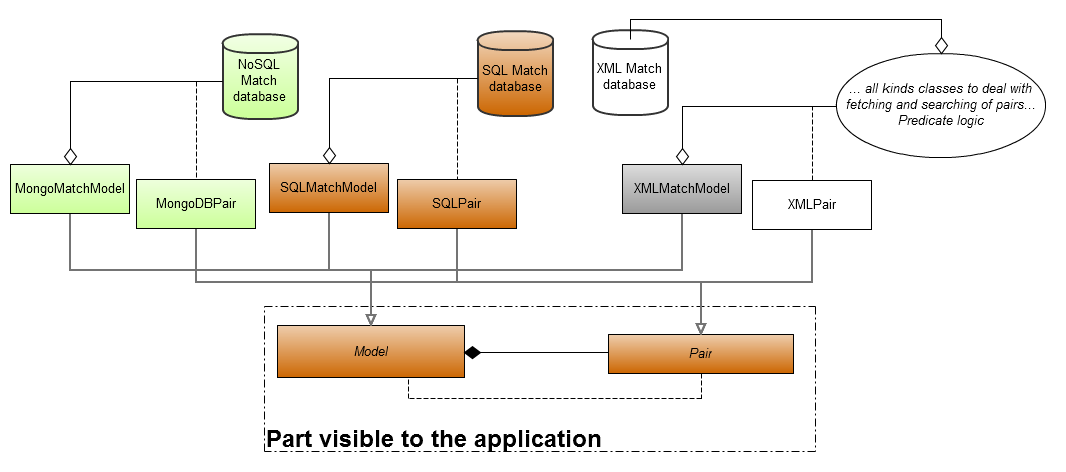
\includegraphics[width=1.0\columnwidth]{images/databaselayer.png}
		\caption{Overzicht van het database systeem, links (groen) is een mogelijke uitbreiding, het middelste deel (oranje) stelt de thesis voor en helemaal rechts (wit) staan de componenten van het thera project.}
		\label{fig:databaselayer}
	\end{center}
\end{figure}

\section{Implementatie}
Ondanks de simpliciteit van de te modelleren data zijn er verscheidene manieren om dit te doen binnen het relationele concept. In figuur~\ref{fig:databasemodel} staat een schematisch model dat moet omgezet worden in SQL tabellen. Het staat buiten twijfel dat tenminste de geschiedenis en de gebruikers in een aparte tabel moeten: voor elk attribuut kunnen er immers verschillende rijen in een geschiedenistabel staan, en meerdere rijen in een geschiedenistabel kunnen door dezelfde gebruiker veroorzaakt zijn. Attributen zouden als kolommen in de ``voorstel'' tabel kunnen gaan, of elk een eigen tabel hebben. De eerste versie komt min of meer overeen met hoe een NoSQL \emph{document} database dit zou voorstellen. Het voordeel van de kolom-aanpak (die \emph{de}normaler is dan de tabel-aanpak) is grotere snelheid bij het opvragen (geen JOINs\footnote{Het commando om twee tabellen met elkaar te verbinden heet een JOIN in SQL. Hoewel de database dit expliciet voorziet en opsplitsen in tabellen aangemoedigd wordt, is het verbinden van veel tabellen vaak nefast voor de performantie.}) en het neemt minder ruimte in op de harde schijf omdat er geen verwijzingen moeten bijgehouden worden voor elk attribuut. Het laatste voordeel voert de snelheid nog eens op want er kan zo meer data in het werkgeheugen blijven. Anderzijds laat de tabel-aanpak toe om attributen te defini\"eren die niet voor alle fragmentparen bestaan, bijvoorbeeld als slechts 1000 van het miljoen paren een commentaar bevat. Op die manier kan afhankelijk van de verdeling van de attributen zelfs nog meer ruimte bespaard worden. SQLite, de implementatie voor kleine lokale kopie\"en kan ook geen kolommen verwijderen van een tabel. Omdat het eenvoudig is de tabel-aanpak om te zetten in de kolom-aanpak is deze preferibel om te beginnen. De eigenlijk beslissing kan uitgesteld worden tot wanneer blijkt dat er performantieproblemen zijn.\\

\begin{figure}[ht]
	\begin{center}
		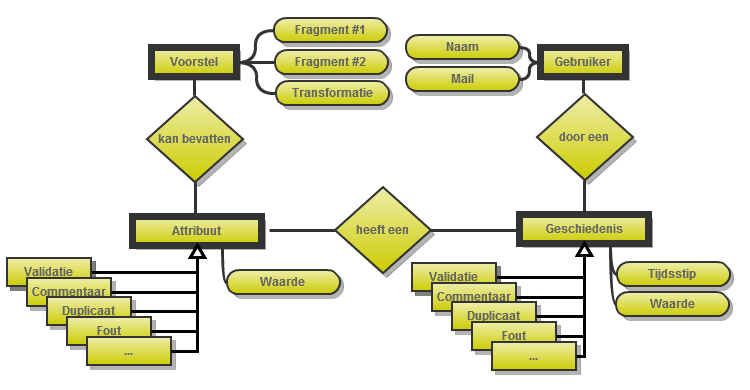
\includegraphics[width=1.0\columnwidth]{images/databasemodel.png}
		\caption{Een relationele modellering van de data}
		\label{fig:databasemodel}
	\end{center}
\end{figure}

\subsection{Normale attributen}
Dit model heeft een groot voordeel: het is voorspelbaar maar uitbreidbaar. De voorspelbaarheid van het attribuut-formaat zorgt ervoor dat queries automatisch kunnen gegenereerd worden, omdat elk veld aan een specifieke structuur voldoet. Steeds is het mogelijk om attributen toe te voegen en te verwijderen: de databaselaag ``herkent'' elke tabel die eruitziet als een attribuut en brengt alle ge\"interesseerde componenten hiervan op de hoogte.

\subsection{Complexe attributen}
De (verplichte) voorspelbaarheid van de attributen kan ook op een dwangbuis lijken: er is zeker informatie denkbaar die niet simpelweg in \'e\'en kolom past of gaat over meer dan \'e\'en paar tegelijkertijd. In extremis is het mogelijk om dit soort data toe te voegen en te onderhouden door een module te schrijven. Er bestaan dan tabellen waarmee de databaselaag niet kan werken, maar de module kan wel via ruwe queries aan die data. Dit heeft natuurlijk het nadeel dat een heel deel van de infrastructuur op die manier ontweken wordt. Andere modules kunnen deze data niet ``ontdekken'' en weergeven en de queries worden niet automatisch geoptimaliseerd. Filters en sorteeroperaties zijn dan ook niet toegankelijk via de normale interface.\\

Een oplossing hiervoor zijn meta-attributen. Deze zijn niet schrijfbaar omdat ze opgemaakt zijn uit samengestelde data van andere tabellen. Voor de rest gedragen ze zich exact zoals normale attributen. Dit wil zeggen dat ze automatisch kunnen ontdekt en gebruikt worden. Het beste hieraan is dat dit allemaal in de declaratieve taal van de database kan gebeuren, waardoor extra modules of een hercompilatie van het programma niet nodig zijn.\\

Deze functionaliteit wordt ge\"implementeerd met behulp van SQL Views, een manier om een verzoek als een tabel voor te stellen. Als er een verzoek op onregelmatig gevormde data kan gemaakt worden dat \textbf{lijkt} op een attribuut, kan dit een meta-attribuut zijn. Om de zojuist beschreven zaken wat minder abstract te maken, volgt een voorbeeld van een twee echte meta-attributen:\\

\subsubsection{Duplicaten}
De automatische herkenners stellen soms paren voor die hard op elkaar gelijken maar niet exact dezelfde zijn (zie figuur~\ref{fig:duplicates}). Om data-analyse redenen worden deze niet automatisch verworpen, ze hebben licht verschillende eigenschappen en het kan nuttig zijn deze te onderzoeken.\\

\begin{figure}[ht]
	\begin{center}
		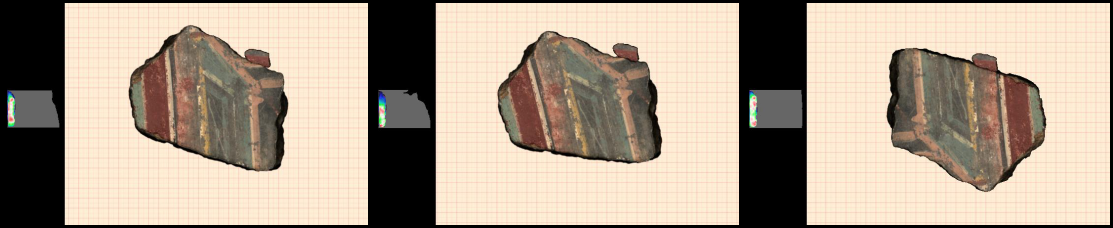
\includegraphics[width=1.0\columnwidth]{images/duplicates.png}
		\caption{Duplicaten: het tweede paar is een duplicaat van het eerste, het derde niet.}
		\label{fig:duplicates}
	\end{center}
\end{figure}

Als men niet specifiek op zoek is naar duplicaten, is het dikwijls beter om enkel het beste paar uit een groep duplicaten te laten zien. Tegelijkertijd moet de gebruikersomgeving een visuele hint kunnen geven dat een bepaald voorstel enkele duplicaten heeft. Opslaan welk paar representatief is, kan nog voorgesteld worden als een attribuut. De waarde van dit attribuut, ``duplicaat'' genaamd, is een verwijzing naar het representatieve paar van de groep of het getal 0. Als de waarde 0 is, geeft dit aan dat een paar de beste uit zijn groep is (elk paar is dus in het begin de beste uit de groep die alleen het paar zelf bevat). Als men wil aanduiden dat een groep paren een duplicaat is van een ander, volstaat het om de waarde van hun ``duplicaat''-attribuut op het identificatienummer van dit paar te zetten.\\

Er is slechts \'e\'en probleem over: door te kijken naar het ``duplicaat''-argument kan men niet weten of dit paar duplicaten heeft of niet (enkel of het een duplicaat of een representatief paar is). Op het eerste zicht lijkt het nodig een apart attribuut ``aantal\_duplicaten'' bij te houden en dit telkens aan te passen als er ergens een in ``duplicaat'' een verwijzing veranderd. Dit is mogelijk maar zeer gevoelig voor corruptie (desynchronisatie van beide tabellen). Eigenlijk kan het aantal duplicaten rechtstreeks uit het ``duplicaat''-attribuut worden gehaald: voor het paar waarvan men wil weten of het een duplicaat heeft, tel hoeveel ernaar verwijzen. Een apart attribuut bijhouden zou dus redundant zijn. Deze telsom valt in een SQL-verzoek te vertalen:

\lstinputlisting[label=code:duplicates,caption=Deze query kan als view dienen om het aantal duplicaten per paar als meta-attribuut te gebruiken, language=SQL]{source/duplicates.sql}

De databaselaag kan van deze zin een meta-attribuut maken dat aangeeft hoeveel duplicaten een paar heeft. Het gedraagt zich als een extra tabel maar is in feite gewoon een datatransformatie. De \emph{MatchTileView} module die later wordt besproken kiest ervoor om dit meta-attribuut weer te geven door een paar laagjes onder een afbeelding van het paar te tekenen, zoals in figuur~\ref{fig:duplicatesdone}.

\begin{figure}[!h]
	\begin{center}
		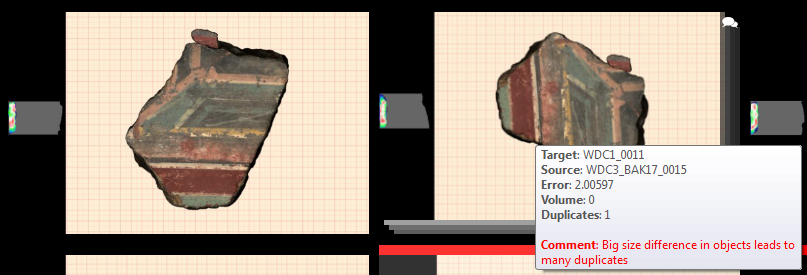
\includegraphics[width=1.0\columnwidth]{images/duplicates-2.png}
		\caption{Duplicaten: het tweede paar van figuur~\ref{fig:duplicates} verwijst nu naar het eerste paar}
		\label{fig:duplicatesdone}
	\end{center}
\end{figure}

\subsubsection{Correspondentie}
Een ander voorbeeld van een meta-attribuut is correspondentie. Alle commentaren die ooit op een fragment zijn gegeven kunnen aan elkaar worden gezet! Een voorbeeld van een query die hiervoor kan dienen is broncode~\ref{code:correspondence}\\

\lstinputlisting[float=htpb,label=code:correspondence,caption=Deze query kan als view dienen om de geschiedenis van een ``commentaar''-attribuut om te vormen tot een ``correspondentie''-attribuut, language=SQL]{source/correspondence.sql}

Zo zijn er nog vele andere meta-attributen denkbaar, er is geen beperking op hoeveel tabellen er moeten gecombineerd worden om het te verkrijgen zolang het resultaat maar de vorm van een normaal attribuut heeft.

\subsection{Querygeneratie}
Omdat verschillende modules en bij extensie gebruikers andere noden hebben, worden de verzoeken naar de database steeds opnieuw gegenereerd uitgaande van een stel parameters.\\

De eerste iteratie van het systeem was zeer eenvoudig: een query bestond uit een sorteerveld, sorteerrichting en een enkele filter op een attribuut. Dit werkte acceptabel voor kleine collecties zoals degene waar Browsematches en Griphos mee moeten werken, maar was niet echt vernieuwend.\\

Een aanzienlijk probleem was bijvoorbeeld dat alle fragmenten die voldeden aan de filtercriteria werden opgehaald. Een duizendtal paren van een SQL implementatie die lokaal draait (of zelfs volledig in het geheugen, zoals SQLite) is snel. Tienduizenden paren gaat niet meer zo vlot. Niet alleen nemen die veel geheugen in, de informatie in het verzoek moet elke keer verwerkt worden en omgezet in evenveel C++ objecten. Dit is vooral traag omwille van de opslag van de transformatiematrix als pure tekst, die telkens omgezet wordt naar een matrix van (32-bit) decimale getallen. De tekstopslag laat arbitraire precisie toe, wat belangrijk is om het voorstel van de automatische herkenner zo getrouw mogelijk te maken. De volgende subsecties bespreken eerst hoe filters mogelijk zijn en daarna enkele optimalisaties die het systeem effici\"ent maken voor grote datasets en over (trage) netwerkverbindingen.

\subsubsection{Filters}
In hoofdstuk~\ref{hoofdstuk:ontwerp} werd reeds uit de doeken gedaan dat er meerdere filters tegelijkertijd mogelijk zijn. Alle attributen zitten opgeslagen in aparte tabellen, in SQL moet een query deze expliciet vermelden. Aangezien de filters willekeurige tekst zijn die hopelijk welgevormde SQL voorstellen, is een tekstanalyse nodig om te bepalen op welke attributen ze steunen. Dit wordt gedaan met reguliere expressies\footnote{Een formele taal die het mogelijk maakt om ingewikkelde patronen in tekst te herkennen.}. Alle filters worden conjunctief (met het ``AND'' sleutelwoord) in een WHERE-clausule gezet en alle ontdekte afhankelijkheden worden met een ``JOIN'' in het domein gebracht.\\

Merk op dat indien eerder de kolom-aanpak --- d.w.z. alle attributen als extra kolommen in de parentabel --- was genomen, deze tekstanalyse niet nodig zou geweest zijn. Gelukkig blijkt de analyse nuttig voor andere optimalisaties die hieronder worden beschreven. 

\subsubsection{Standaardisatie}
Ondanks het feit dat SQL een gestandaardiseerde taal is, gebruikt elke implementatie wel een eigen dialect. Daarom loopt een preprocessor steeds door de volledige query om de dialecten te unificeren, ook hiervoor worden reguliere expressies ten volle benut.

\subsubsection{Paginatie}
Tienduizenden paren ophalen werd al aangegeven als een oorzaak van traagheid, zelfs op lokale installaties. Hetzelfde probleem doet zich nog veel erger voor als de verbinding naar de database over het netwerk loopt. Zonder de effici\"entieverliezen van de databaseopslag neemt elk paar zonder attributen ongeveer 924 bytes in\footnote{Het grooste deel hiervan is afkomstig van de tekstvoorstelling van de transformatiematrix}. Het is niet ongewoon om verzamelingen van 10000 paren te weerhouden, wat een ondergrens van 8.8MB over het netwerk zou betekenen. Een redelijk doel lijkt om alle verzoeken binnen een seconde af te werken, wat niet mogelijk is met zulke hoeveelheden data.\\

Om die reden zal het model bijna nooit de volledige set aan de database opvragen, maar slechts een klein deeltje. Allereerst wordt aan de database gevraagd hoeveel paren aan de criteria voldoen, zodat het model kan rapporteren dat het X aantal paren in bezit heeft. Dit laadt ook meteen veel noodzakelijke data in het werkgeheugen van de server. Als een component dan vraagt om een bepaald paar, zal het model kijken of de aanvraag binnen het bereik van het huidige venster past. Indien niet, wordt het venster opgehaald waarin de aanvraag wel past. Dit proces is transparant voor de componenten die van het model gebruik maken. Ze kunnen de parameters zoals venstergrootte wel be\"invloeden door hints te geven, hoewel het model niet verplicht is deze te volgen. Dit is vooral handig voor componenten die een willekeurig toegangspatroon naar de data hebben, waarvoor vensters bijzonder ineffici\"ent zijn omdat er bij elke aanvraag een volledig nieuw venster opgehaald wordt.

\subsubsection{Voorladen}
Een component kan aan een fragmentpaar vragen welke waarde het heeft voor een bepaald attribuut. De eerste versies van zo'n fragmentpaar-objecten vuurden een query af naar de database elke keer een attribuut opgevraagd werd. Dit is eenvoudig en zorgt ervoor dat de waarde altijd zo actueel mogelijk is. De query op zich is bijzonder eenvoudig en kan razendsnel afgehandeld worden door de database. In een venster van de belangrijkste module passen 20 fragmentparen. De module heeft van elk paar ongeveer 5 attributen nodig om weer te geven, dit geeft 100 extra verzoeken aan de database na het ophalen van de paren zelf. Voor een lokale server is dit geen probleem, maar als de verzoeken over het netwerk moeten komt er tenminste 100 maal de heen-en-weer tijd van een netwerkpakket bij.\footnote{Queries worden niet parallel uitgevoerd}\\

Onafhankelijk van de snelheid van het verzoek maakt deze techiek werken over het netwerk te traag. Om die reden beschikt elk fragmentpaar over een datastructuur waarin het eerst zal kijken of het geen lokale kopie van het attribuut heeft. De querygenerator werd voorzien van de capabiliteit om een parameter ``voorlaadvelden'' aan te nemen, die ervoor zorgt dat een paar reeds voorgevuld wordt met de gevraagde attributen. Het aantal queries per venster loopt dan terug naar 1. Dit heeft geen impact op de versheid van de data, de attributen worden in ieder geval slechts bij het laden van het venster opgevraagd.

\subsubsection{Geforceerde indexen}
Een index is een versnellingsstructuur die de database toelaat om niet de volledige collectie af te gaan bij elk verzoek. Meestal gaat het hier over een binaire boom die ervoor zorgt dat queries op exacte waarden en bereiken (vb. $error < 0.50140$ $\land$ $error > 0.45713$) zeer snel gaan. Indexen zijn gedefinieerd per kolom of groepering van kolommen, het voorbeeld van daarnet heeft dus een index op de ``error'' kolom nodig. Dit is \'e\'en van de zaken die het predicaten-systeem van het thera project mistte.\\

De query planner van MySQL en SQLite is niet zo geavanceerd als die van de commerci\"ele databases, en maakt daarom nogal eens grove fouten als het aankomt op het kiezen van de juiste index. Meer nog, deze twee implementaties zijn gelimiteerd tot \'e\'en index per query, en als deze verkeerd gekozen wordt kan dat soms desastreuze gevolgen hebben voor de snelheid. Om deze cruciale beslissing te maken kijken zij vooral naar de selectiviteit. Samengevat: de query planner kiest over het algemeen de index voor de conditie die de dataset hopelijk het meest verkleint. Als er geen condities maar er wel een gesorteerd resultaat is aangevraagd, zal de planner een index gebruiken om te sorteren als die bestaat (binaire bomen worden gesorteerd bijgehouden).\\

Het probleem is dat deze heuristiek geen rekening houdt met een paar belangrijke zaken. Stel een database met een miljoen paren voor en een conditie in een query brengt dit terug naar een half miljoen, dit half miljoen is niet gesorteerd. Indien er toch gesorteerd moet worden, moet dat in situ gebeuren, zonder een index. Dit is reeds zeer traag op zich. Daarbovenop past zo'n resultaat niet in het werkgeheugen, dus de database sorteert in stukjes door het resultaat weg te schrijven naar het bestandssysteem. Dit gebeurt allemaal ondanks het feit dat er uiteindelijk slechts enkele paren gaan opgevraagd worden.\\

Daarom is het beter om in dit geval selectiviteit te laten voor wat het is en een index te gebruiken om het resultaat reeds gesorteerd op te vragen. Op die manier moet er geen tijdelijk bestand aangemaakt worden. De querygenerator van dit project is geavanceerd genoeg om te detecteren wanneer het beter is om een sorteerindex te forceren en doet dit ook.

\subsubsection{Snelle paginatie}
Paginatie is goed om de hoeveelheid getransfereerde data te minimaliseren, maar de simpele vorm is traag voor grote databases gecombineerd met vensters ver in de dataset. Zo kan een query die voor venster $[100, 120]$ nog binnen de 50 milliseconden afgewerkt kan worden, plots 7000 milliseconden duren voor venster $[10000, 10020]$. De reden heeft onder andere te maken met het feit dat voor de tweede query alle 10000 rijen die niet moeten opgehaald worden toch worden nagekeken. De database kan niet op voorhand weten welke rij precies de 10000'ste is onder de geldende criteria. Bij grote databases is het erg waarschijnlijk dat deze 10000 rijen niet in elkaars buurt staan op de harde schijf, wat de lange zoektijd verklaart.\\

Een oplossing is om de database contextinformatie mee te geven~\cite{sqlfastpag}. Als het vorige opgevraagde venster afdalend gesorteerd was op de \emph{fout}, dan zal het volgende venster beginnen met een \emph{fout} kleiner of gelijk aan de fout van het einde van het huidige venster. Door dit mee te geven in conditie kan de database gebruik maken van een index en zo de opvraagtijd dramatisch inkorten. Voor dit project is deze techniek uitgebreid geweest naar een krachtigere variant die ``relatieve positionering'' werd gedoopt. Dit wil gewoon zeggen dat de querygenerator altijd de meest dichtbijzijnde gekende waarde zal gebruiken om een nieuw venster op te halen.

\subsubsection{Late rijopzoeking}
Late rijopzoeking is uiteindelijk de meest effectieve optimalisatie van allemaal. Het maakt sommige queries zo snel dat het effect van de andere optimalisaties niet meer te merken is. E\'en van de voornaamste redenen waarom queries traag zijn is dat elke keer er een waarde uit een rij nodig is, alle gevraagde kolommen worden opgehaald, of de rij nu in het uiteindelijke resultaat zit of niet. Als het veld dat nagekeken moet worden een simpel geheel getal is van 4 bytes, is het bijzonder kwistig om meteen nog eens een slordige 1000 bytes aan misschien onnodige informatie op te halen. Om de zaken erger te maken staan deze 1000 bytes met grote kans opnieuw niet dicht bij elkaar op de harde schijf\footnote{Dit proximiteitsargument is niet van toepassing op \emph{Solid State Drives}}, wat voor hoge zoektijden zorgt.\\

Dit slecht gedrag ontwijken kan door middel van een subquery. Het basisidee is: de binnenste query reduceert de dataset zoveel mogelijk en haalt enkel de nodige informatie op om de correcte rijen te identificeren (een sleutel). De buitenste query haalt dan al de nodige informatie op aan de hand van die sleutel. Met een venster kunnen er dus nooit meer rijen volledig opgehaald worden dan de venstergrootte.\\

Om de binnenste query zo effici\"ent mogelijk te maken is het voordelig te weten welke velden en tabellen nodig zijn om de dataset te reduceren en welke kunnen doorgeschoven worden naar de buitenste query. Dat is waar de afhankelijkheidsanalyse van daarstraks goed van pas komt.\\

Normaalgezien zou de queryplanner van de database deze optimalisatie zelf moeten uitvoeren, maar zowel SQLite, MySQL en verassend genoeg PostgreSQL\footnote{De queryplanner van PostgreSQL staat bekend als een van de meest geavanceerde, en zou zelfs specifiek late rijopzoeking ondersteunen.} leken hier (veel) voordeel bij te halen.

\subsubsection{Experimenteel: materialized views}
Een spijtig nadeel van de kracht van meta-attributen is dat ze queries sterk vertragen. Hun dynamische aard zorgt ervoor dat de achterliggende query steeds wordt uitgevoerd voor elk verzoek. Een rij ophalen van ``aantal\_duplicaten'' impliceert op die manier een volledige scan de ``duplicaat'' tabel. Vele oplossingen voor dit probleem werden getest maar geen enkele bracht de nodige verbetering of waren slechts van toepassing op een beperkte subset van de mogelijke verzoeken. Het enige wat overbleef was doen wat meta-attributen net proberen te vermijden: een echte tabel maken van de view. Natuurlijk moest dit gebeuren zonder de nadelen van een echte tabel die niet gedesynchroniseert kan geraken met de originele tabellen.\\

Het concept op zich heet een gematerialiseerde view. De opzet is om een automatische verbinding te maken tussen de moedertabellen en het meta-attribuut, zodat elke update gepropageerd wordt. Dit is een simpel uitgangspunt, maar heeft een verassend moeilijke uitwerking. De huidige implementatie is zeer rudimentair en werkt alleen in PostgreSQL, de implementatie met de meest geavanceerde programmeermogelijkheden. De resultaten zijn echter veelbelovend, zie sectie~\ref{sec:benchmarks}.

\subsection{Collaboratie}
De verschillende optimalisaties uit de vorige secties maken het mogelijk om een externe database te gebruiken en toch met grote snelheid te navigeren in de dataset. Dit betekent dat iedereen steeds de meeste actuele data te zien krijgt. In deze opstelling is synchronisatie niet nodig, zolang er een netwerk- of internetverbinding beschikbaar is. Als meerdere gebruikers tegelijkertijd met dezelfde paren aan het werken zijn, zullen ze elkaars veranderingen niet zien verschijnen tot ze het venster vernieuwen. Voor deze situatie is een oplossing gemaakt die gebruikmaakt van het feit dat de meeste queries snel afgehandeld worden. Als het model merkt dat het ophalen van een venster snel gaat, zal het periodisch proberen dit venster te vernieuwen. De periode past zich aan de omstandigheden aan, hoe langer het duurt om een venster op te vragen, hoe langer het model zal wachten. Dit is zo omdat de reden voor de traagheid misschien een overbelasting van de database is.\footnote{Ge\"inspireerd door het dynamisch gedrag van het TCP pakketprotocol}\\

Dankzij dit systeem verschijnen de laatste nieuwe veranderingen steeds op het scherm van de gebruiker, zodat geen dubbel werk wordt verricht.

\section{Data mining}
Maak ketting van (yes+maybe) ---> zoek naar alle buren binnen 1 hop (algoritme is geschreven) --- FINDNEIGHBOURS.SQL

Meer mogelijkheden: geef alle paren die recent zijn aangepast.


\section{Benchmarks}
\label{sec:benchmarks}
Er zijn reeds een paar namen gevallen van gebruikte database implementaties: SQLite, MySQL en PostgreSQL. In het begin draaide 
Dankzij de flexibiliteit die nodig was om zowel SQLite als MySQL het grootst mogelijke deel van de code te laten delen

\subsection{Indexering}
Analyse van datatoegangspatroon: vooral SELECT, ORDER BY, GROUP BY ---->
veelvuldig gebruik van indexes

optimize voor fast reads -----> inserts kunnen lokaal gedaan worden, updates hopelijk niet zo veel of lokaal


\subsection{Opstelling}
Beide databases kregen 512 MB RAM aan werkgeheugen toe. Het is natuurlijk niet mogelijk om exact dezelfde configuratie te krijgen omdat de opties verschillen.

De query cache staat af
Om de variabiliteit van de filesystem (nederlands) cache een beetje buiten spel te zetten zijn al deze routines ``opgewarmd''

Pagination
Late row lookup

Ideaal = minder dan een seconden voor elke gegeven query vanuit een gebruikersinteractie standpunt (System Response Time and User Satisfaction pagina 5)

Effect van DB configuratie (veel geheugen\ldots)

Suggested workaround voor het text probleem -> sphinx, restrict fragment names (niet ZO gemakkelijk), string + nummer
Suggested workaround voor het indexing probleem (zoals gezien voor status IN (\ldots)) -> force een index?! dunno\ldots hij pakt in ieder geval de verkeerde!

'High Performance MySQL', Second Edition, O'REILLY, ISBN: 978-0-596-10171-8
MySQL Reference Manual for version 5.1

http://nlp.stanford.edu/IR-book/html/htmledition/permuterm-indexes-1.html (dit is hoe wildspeed werkt) (LIKE performance lijkt niet zo slecht in Postgres, het is de sorting eerder\ldots)
http://www.slideshare.net/techdude/how-to-kill-mysql-performance
http://stackoverflow.com/questions/1540590/how-to-speed-up-like-operation-in-sql-postgres-preferably <--- use trigrams (fail), MAAR BETER IN 9.1 (future research)
https://cgsrv1.arrc.csiro.au/blog/2010/06/23/materializedindexed-views-for-postgresql/
\chapter{Synchronisatie}
\label{hoofdstuk:synchronisatie}
Het thera project bestaat al een tijdje en er zijn reeds vele XML-bestanden met validaties van voorstellen in omloop. Ondanks de eventuele overgang van het oude naar het nieuwe systeem is het belangrijk dat deze resultaten niet verloren gaan, het heeft immers veel werk gekost om ze te maken. Als bestanden verschillende paren bevatten --- omdat ze bijvoorbeeld door een ander identificatiealgoritme zijn gegenereerd --- maar over eenzelfde opgraving gaan, is het ook nuttig om deze te consolideren. Indien er geen internetverbinding is of even geen storing van anderen wil hebben, kan een lokale kopie ge\"extraheerd en later terug ge\"importeerd worden. Dit alles kan gedaan worden met de synchronisatiecomponenten van dit project.

\section{Opzet}
Om te synchroniseren selecteert men een meester- en een slaaf-database, de conventie is dat de slaaf door de meester zal geabsorbeerd worden. Na het proces heeft de meester alle gewenste veranderingen en blijft de slaaf onveranderd over. Er zijn verschillende fasen (voorlopig 3): \textbf{Gebruikers}, \textbf{Paren} en \textbf{Attributen}. In elke fase krijgt de gebruiker een scherm te zien met daarin de verschillen tussen beide databases, het biedt de mogelijkheid om aanpassingen te maken alvorens naar de volgende stap te gaan. Het is belangrijk gebruikers keuzes te laten maken waarin ze ge\"interesseerd zijn en ze niet lastig te vallen met keuzes die ze niet willen maken, beide zaken negeren leidt tot frustraties~\cite{Joel2001}. De algoritmes proberen daarom steeds een standaardkeuze in te vullen aan de hand van heuristieken, deze kunnen indien gewenst verworpen worden. Als er door gebrek aan informatie geen automatische belissing kan genomen worden, moeten alle conflicten eerst manueel opgelost worden. Figuren~\ref{fig:merge-attrib} en~\ref{fig:merge-choose} tonen hoe deze stappen eruitzien en figuur~\ref{fig:merging-overview} geeft een schematische kijk op het systeem. Sommige SQL-implementaties bieden automatische replicatie aan, dit wordt niet gebruikt omdat het minder flexibel is qua conflictresolutie noch compatibel over implementaties heen.\\

\begin{figure}[ht]
	\begin{center}
		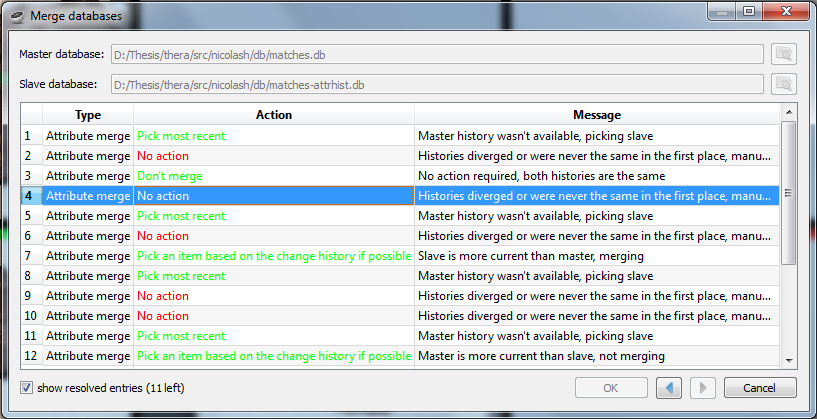
\includegraphics[width=1.0\columnwidth]{images/merge-action-1-small.png}
		\caption{Een uittreksel van de attributen-fase van het synchronisatieproces. ``No Action''  duidt aan dat er geen automatische resolutie toegepast is geweest, hierop dubbelklikken geeft een keuzescherm weer (rechts).}
		\label{fig:merge-attrib}
	\end{center}
\end{figure}

\begin{figure}[ht]
	\begin{center}
		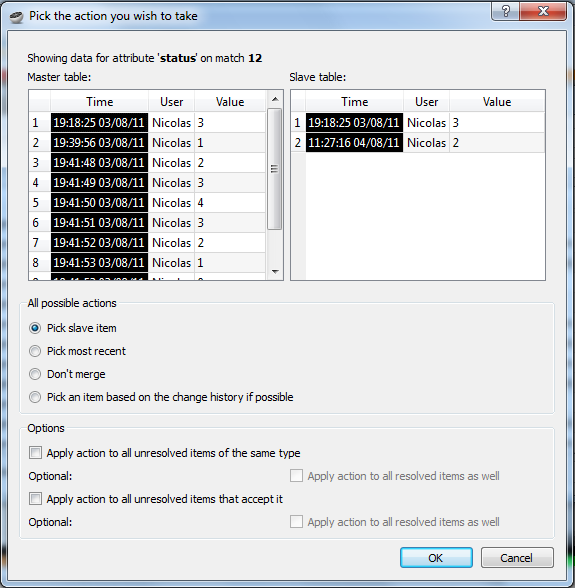
\includegraphics[width=0.5\columnwidth]{images/merge-action-2-small.png}
		\caption{Elk type conflict laat een aantal manieren toe om het op te lossen. Deze figuur beeldt een attribuut-conflict voor.}
		\label{fig:merge-choose}
	\end{center}
\end{figure}

% Het gros van het onderzoek op het vlak van samenvoegingsalgoritmen gaat over het combineren van tekstbestanden, hier werden reeds vele innovatieve aanpakken voor ontwikkeld\footnote{Arbitraire tekst is moeilijk to synchroniseren omwille van de vele vrijheidsgraden, een tekstbestand kan op ontelbare manieren veranderen en het is niet steeds triviaal om te zien hoe twee conflicterende aanpassingen in elkaar moeten gevoegd worden}. Gelukkig vallen vele problemen weg door de eenvoudigere (minder vrije) structuur van de data in dit project. Voor de attributen wordt een geschiedenis bijgehouden. De algoritmen gebruikt voor elke fase worden in de volgende secties uit de doeken gedaan.

\subsection{Paren}
In deze stap worden de voorstellen zonder attributen uit beide databases vergeleken en gesynchroniseerd. Deze objecten bevatten een identificatiecode, twee namen van fragmenten en een 3D-transformatiematrix. De identificatiecode is echter geen uniek gegeven over alle databeses, eerder een manier om effici\"ent naar het object te verwijzen binnen eenzelfde database. Het is echter duidelijk dat als twee voorstellen uit dezelfde fragmenten bestaan en dezelfde transformatie hebben, ze identiek kunnen geacht worden. De aanwezigheid van afrondingsfouten en duplicaten is problematisch. Duplicaten zullen per definitie een gelijkaardige transformatiematrix hebben, hoe ze te onderscheiden van afrondingsfouten? De matrix van een voorstel uit de slaaf-database wordt afgetrokken van de matrix van elk voorstel uit de meester-database dat uit dezelfde fragmenten bestaat, hiervan wordt vervolgens de Frobenius norm\footnote{De euclidische norm van de vector die ontstaat als men de rijen of kolommen van een matrix achter elkaar plaatst.} genomen. Hieruit ontstaat een rij van getallen die aangeven hoe gelijkaardig het voorstel is aan elk van de mogelijke overeenkomstige voorstellen uit de meester-database. Het kleinste getal geeft het meest overeenkomstige paar aan. Indien dit kleinste getal een ordegrootte (10x) kleiner is dan het maximale verschil tussen dit overeenkomstig paar en diens duplicaten, wordt aangenomen dat het de paren in kwestie identiek zijn. Indien niet wordt het paar uit de slaaf-database als een nieuwe paar ingevoerd.\\

De volledige voorstellenlijst van beide databases moet dus nagekeken worden. Eenmaal beiden in het geheugen geladen zijn verloopt het vergelijkingsproces vrij snel (er wordt een hashmap aangemaakt om in constante tijd te kunnen zien welke voorstellen uit dezelfde fragmenten bestaan). Dit wil natuurlijk wel zeggen dat het synchroniseren van pure paren op zich over het internet niet werkbaar is met een database van miljoenen elementen. Gelukkig gebeurt het niet vaak dat onderzoekers paren toevoegen.\\

Paren die overeenkomen worden aan een identiteitsvertaler toegevoegd, waardoor latere fasen weten dat twee verschillende identificatienummers naar hetzelfde object verwijzen. Een paar dat niet gevonden werd in de meester-database wordt niet automatisch ingevoerd maar als een conflict weergegeven. De gebruiker kan gemakkelijk kiezen om dit toch te doen door ``assign new id'' als actie toe te kennen en aan te vinken om dit te doen voor alle gelijkaardige conflicten (zoals in figuur~\ref{fig:merge-choose}). Het alternatief is ``don't merge'', wat ervoor zorgt dat de nieuwe paren niet toegevoegd worden (en genegeerd in de volgende stappen).

\subsection{Attributen}
Het samenvoegen van attributen verloopt op een andere manier. Het is gemakkelijk te detecteren wanneer zich een conflict voordoet, namelijk als de waarden verschillen. Dit conflict oplossen gaat echter niet automatisch, als een \emph{commentaar}-attribuut bijvoorbeeld twee verschillende teksten bevat, welke is dan de juiste? Misschien de meest recente, zeker als blijkt dat een vorige waarde van de meest recente gelijk is aan de minder recente (gemeenschappelijk ouder). Om automatische resolutie te ondersteunen moet er dus een geschiedenislijst bijgehouden worden. Daarnaast kan nog gekeken worden naar de semantische inhoud van het attribuut om eventueel een oordeel te vellen als de geschiedenismethode faalt.

\subsubsection{Gemeenschappelijke ouder}
Indien beide databases voor een bepaald attribuut een stukje geschiedenis delen, is er een kans dat het conflict automatisch opgelost kan worden. Stel dat in een kopie van een database een attribuut veranderd en ditzelfde attribuut is niet aangeraakt in de originele database. In dat geval kan de nieuwe waarde zonder meer overgenomen worden bij synchronisatie. Het kijken naar een gemeenschappelijke ouder om te synchronizeren wordt in de literatuur \emph{3-way merging}~\cite{sync:diff3} genoemd. De zojuist beschreven situatie komt overeen met het meest linkse vak in figuur~\ref{fig:okay-3-way}. Het is de meest voorkomende want uit de grote hoeveelheid paren is de kans klein dat exact dezelfde (in een korte tijdsspanne) bewerkt worden. In het geval dat dit wel zou gebeuren --- het middelste vakje in de figuur --- kan er niet op die manier gesynchroniseerd worden. Hetzelfde doet zich voor als de beide databases geen geschiedenis delen, deze situate wordt voorgesteld door het meest rechtse vakje. Samenvattend kan er dus niet automatisch gehandeld worden als de geschiedenis divergeert ofwel niet gedeeld is.

\subsubsection{Context}
Toch zijn er situaties denkbaar waar er toch een oplossing is. Stel dat de validatiestatus van een bepaald voorstel ``niet geweten'' is en de database wordt gesplitst in database A en B. In database A wordt vervolgens de status op ``misschien'' gezet en in B op ``correct''. Als de synchronisatie afweet van de semantiek van statussen, zal het correct kunnen afleiden dat ``correct'' een krachtiger status is en dit verkiezen. Voor commentaren kan bijvoorbeeld gelden dat het meest recente de bovenhand krijgt. Dit zijn contextbeslissinggen, waarbij de component op de hoogte moet zijn van de betekenis achter de waarden. Dit soort acties kan over het algemeen niet overgezet worden van het \'ene attribuut op het andere, hetgeen aparte routines voor elk contextgevoelig attribuut veronderstelt.\\

Er zijn ook attributen waar dit soort beslissingen niet eenvoudig kunnen genomen worden (bvb. duplicaten), of waarvoor de routines nog niet gemaakt zijn. In dit laatste geval kan er geen automatische resolutie plaatsvinden en moet de gebruiker ingrijpen alvorens verder te gaan. Er zijn heel wat verschillende acties geldig op een attribuut conflict, enkele daarvan zijn: ``pick most recent'', ``prefer user [username]'', ``prefer slave'' en ``don't merge''.

\begin{figure}[ht]
	\begin{center}
		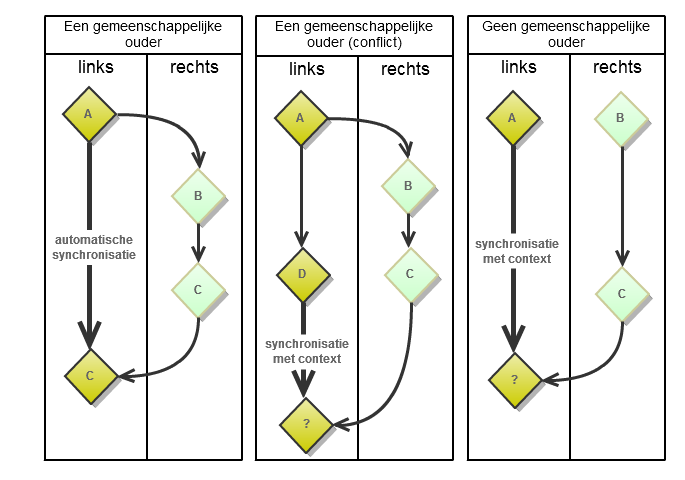
\includegraphics[width=1.0\columnwidth]{images/3-way-merge.png}
		\caption{Situaties waarin automatische resolutie gebaseerd op geschiedenis mogelijk is (eerste figuur) en waar contextinformatie nodig is (tweede en derde figuur). Links is hier gelijk aan de meester-database en rechts is de slaaf-database.}
		\label{fig:okay-3-way}
	\end{center}
\end{figure}

\subsection{Incrementele synchronisatie}
Omdat er een geschiedenis wordt bijgehouden is incrementele synchronisatie voor attributen mogelijk als beide databases geschiedenis delen. De geschiedenis wordt voor elk attribuut apart bijgehouden dus de gemakkelijkste en meest robuuste oplossing is om per attribuut een binair zoekalgoritme te laten zoeken naar het laatste gemeenschappelijke punt. In feite is dit hetzelfde algoritme als hetgene dat gebruikt wordt om de gemeenschappelijke ouder te vinden, met het verschil dat er is deze versie naar alle paren wordt gekeken in plaats van slechts \'e\'en. Dit is robuust omdat er veel verschillende manieren zijn om databases te kopi\"eren en er dus niet kan vertrouwd worden op het aanwezig zijn van splitindicatoren. Enkel de kost van het binair zoeken en het overzetten van de veranderde attributen is dan van belang. Op een database van 50000 paren kan dit een groot verschil opleveren als er bijvoorbeeld slechts 100 attributen veranderd zijn. Op die manier wordt synchroniseren over het internet mogelijk. 
\chapter{Modules}
\label{hoofdstuk:modules}
In dit hoofdstuk komen de voor dit thesisproject ontwikkelde modules aan bod. Zij proberen elk de collectie paarvoorstellen op een andere manier voor te stellen om een beter overzicht te cre\"eren of sneller individuele paren te beoordelen.\\

Modules kunnen ervoor kiezen het model dat ze toegewezen krijgen te manipuleren of niet. Indien wel, zullen alle modules die dit model delen steeds de veranderingen volgen.

\section{MatchTileView}

\begin{figure}[!h]
	\begin{center}
		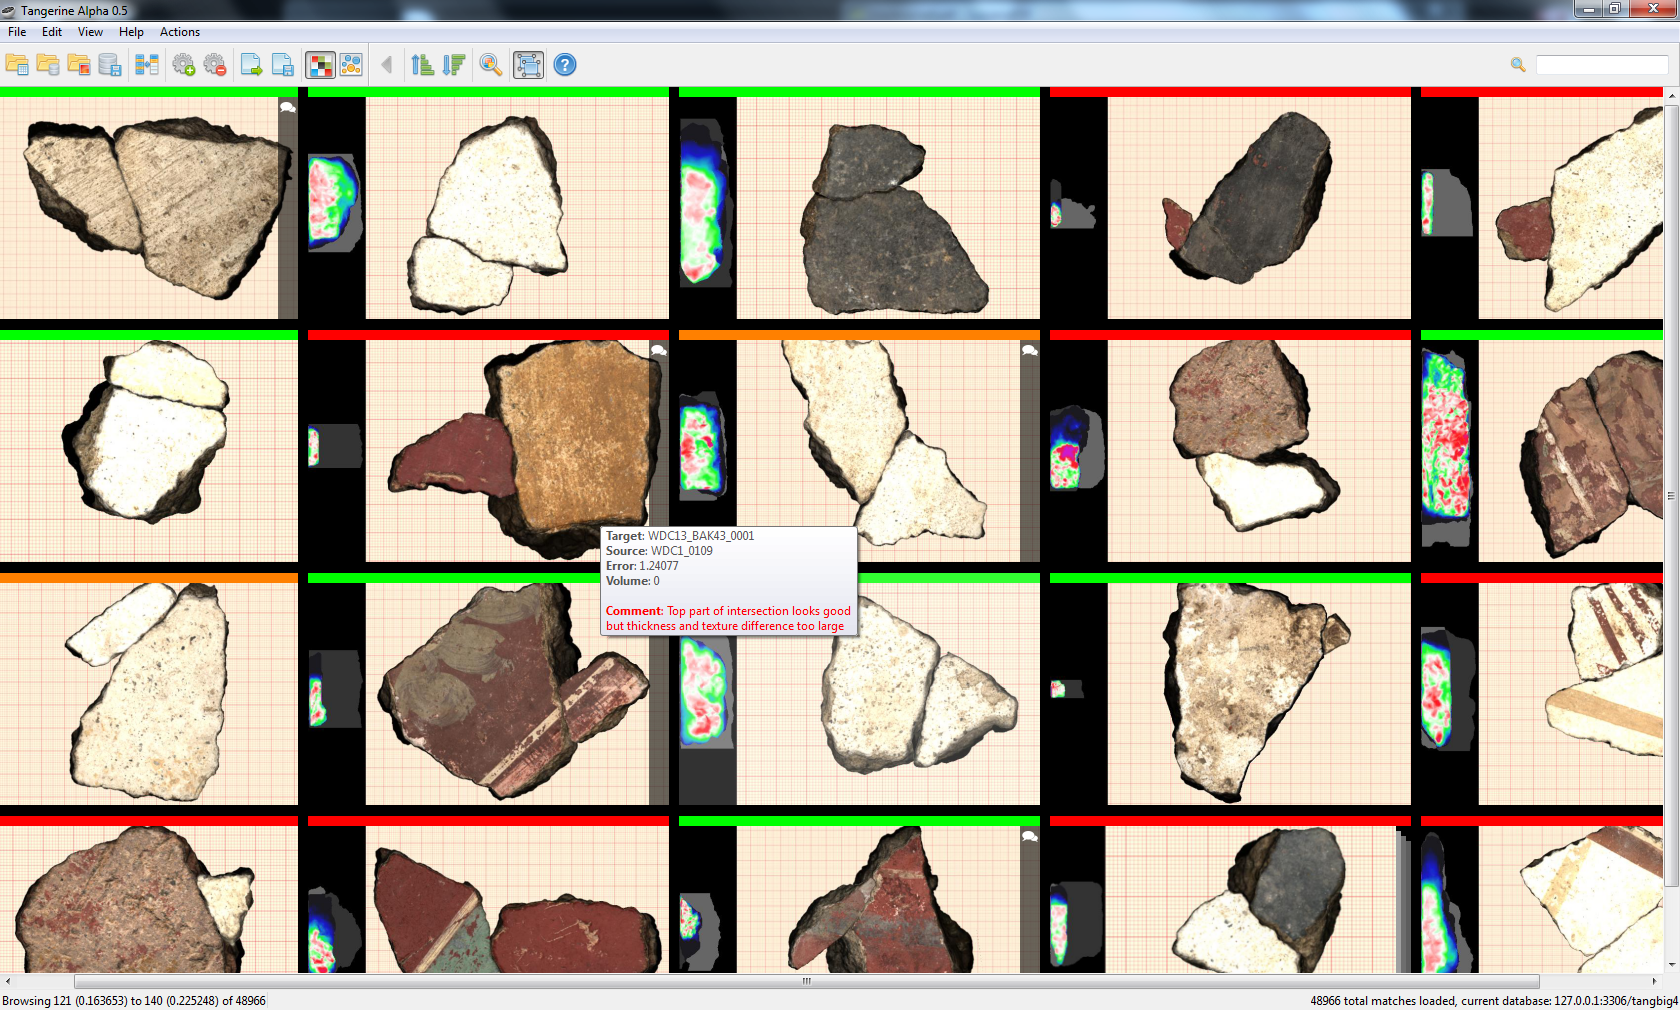
\includegraphics[width=1.0\columnwidth]{images/matchtileview-nice-01.png}
		\caption{De \emph{MachTileView}-module}
		\label{fig:mtv1}
	\end{center}
\end{figure}

\emph{MatchTileView} is de meest uitgewerkte module en stelt de gebruiker in staat om op effici\"ente wijze te zoeken naar de gewenste paren. De manier waarop het die weergeeft is gebaseerd op Browsematches: een dambordpatroon van paren met aan de linkerkant de doorsnede van hun raakvlak en vanboven een kleurcode die aangeeft wat de huidige validatie is\footnote{Groen: zeker correct, Oranje: misschien correct, Rood: zeker niet correct, Grijs: in conflict, Zwart: niet gekend}. De doorsnede is roder/paarser op plaatsen waar de volumes van de fragmenten dieper in elkaar snijden, wit waar ze op elkaar passen en blauwer hoe verder ze uit elkaar staan. Uit ervaring blijkt dat de doorsnede relevant is om te beslissen of een paar interessant is~\cite{Brown2010}. Als men in de realiteit fragmenten op elkaar past, is het natuurlijk niet mogelijk om de doorsnede te bekijken, met als gevolg dat dit nuttige perspectief alleen virtueel te verkrijgen valt. Om deze reden kan de module optioneel enkel de doorsnedes weergeven, waardoor er veel meer paren op een scherm passen (zie figuur~\ref{fig:tileview-reduced-compare}). De aanwezigheid van bepaalde attributen, zoals commentaren of duplicaten, worden visueel weergegeven met iconen en andere tekenstijlen.\\

Met de pijltoetsen kunnen gebruikers navigeren in de verzameling, de statusbalk geeft steeds weer op het hoeveelste scherm men zit en hoeveel paren er aan de huidige criteria voldoen. Er is een werkbalk waarin gebruikers kunnen kiezen op welke eigenschappen er gesorteerd en gefilterd moet worden. Sommige operaties zoals duplicaten uitzetten en verschillende validaties weergeven worden zo frequent toegepast dat ze een eigen knop krijgen op de werkbalk.\\

\begin{figure}[ht]
	\begin{center}
		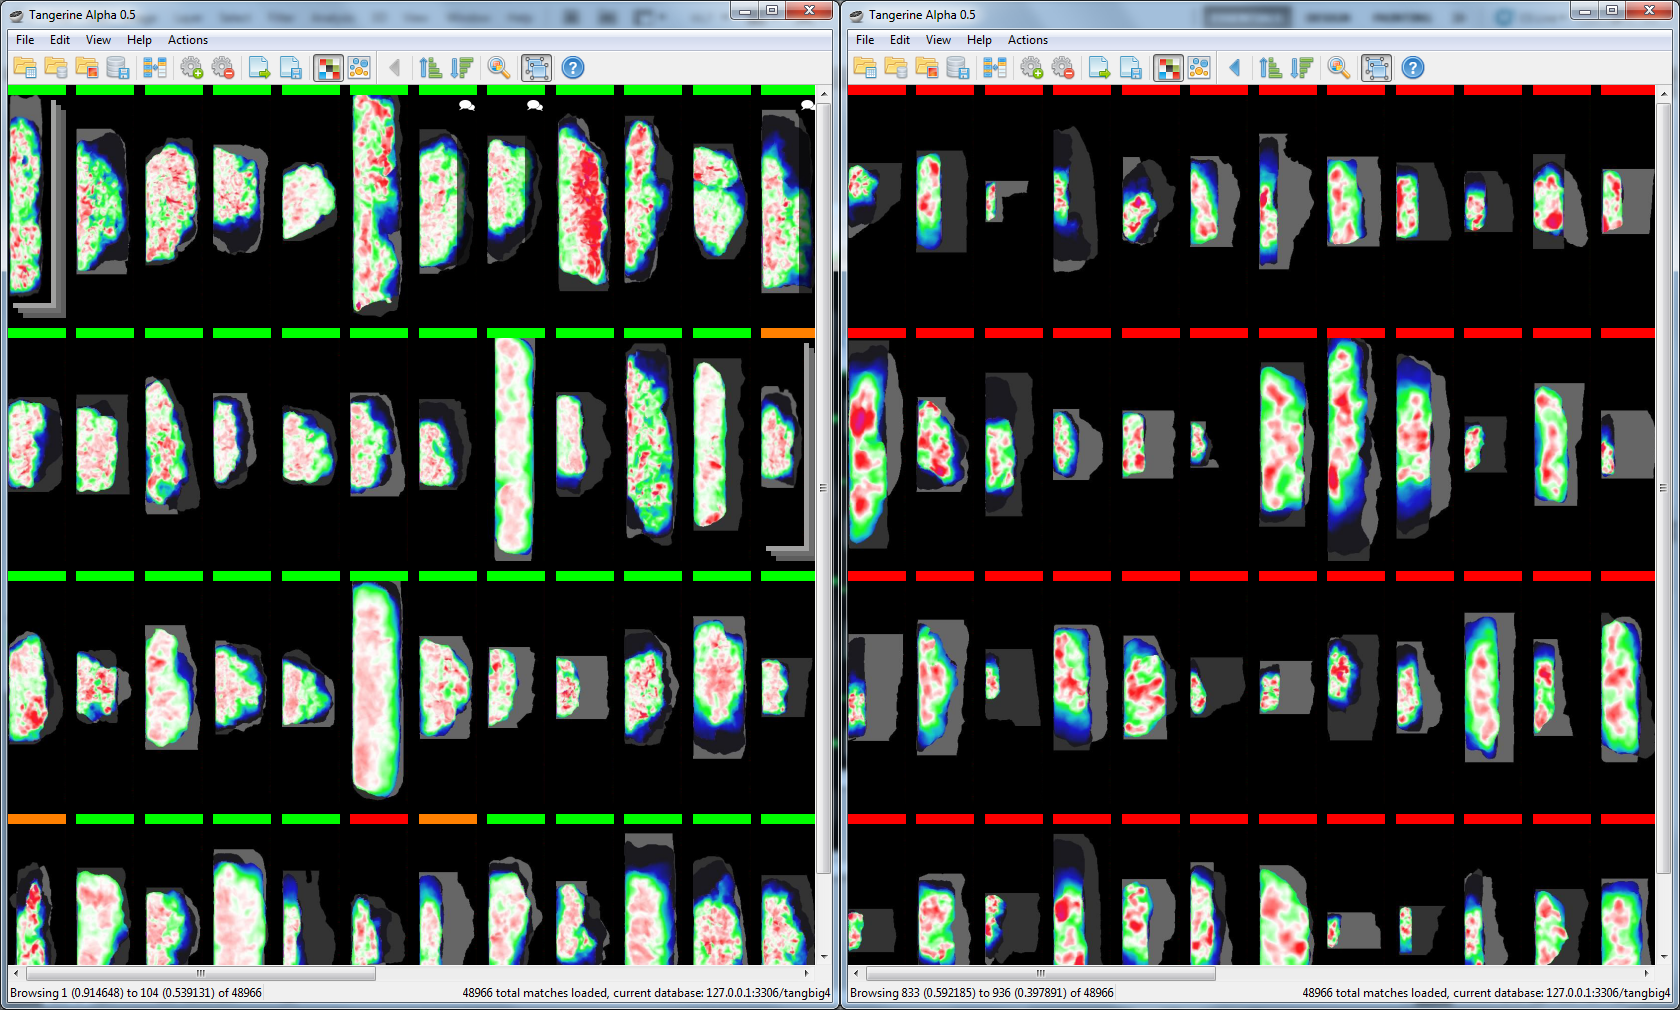
\includegraphics[width=1.0\columnwidth]{images/tileview-reduced-compare-01.png}
		\caption{De doorsnedes van goede paren tegenover die van slechte paren. Een mens kan met ervaring leren om hieruit reeds veel af te leiden. Yassine Ryad bewees dat een algoritme kan gemaakt worden dat deze informatie in een rangschikking omzet.~\cite{Ryad2011}}
		\label{fig:tileview-reduced-compare}
	\end{center}
\end{figure}

In het rechterklikmenu bevinden zich een aantal geavanceerdere filtermogelijkheden die van toepassing zijn op een paar: 

\begin{packed_itemize}
  \item vind alle buren van het paar
  \item vind alle buren van het paar die ermee conflicteren
  \item vind alle buren van het paar die er niet mee conflicteren
  \item vind alle buren van het paar die er niet mee conflicteren en ook niet met elkaar conflicteren
\end{packed_itemize}

Een conflict komt voor als een deel van de rand van een fragment door twee verschillende fragmenten ingenomen wordt. Het kan best zijn dat twee fragmenten niet op dezelfde plaats aansluiten op een andere fragment, maar wel onderlinge volumeintersecties hebben. Dit soort conflicten ook in acht nemen is een toekomstige onderzoeksrichting. De voornoemde operaties zijn vooral handig op voorstellen die reeds te boek staan als \emph{correct} (of zelfs \emph{misschien correct}). De conflicterende buren kunnen bijvoorbeeld onmiddellijk verworpen worden. Tussen de buren die niet conflicteren kan mogelijk een interessant paar zitten. \\

De laatste optie stelt een cluster rond het geselecteerde paar op. Het proces gaat als volgt: de database wordt gevraagd naar alle buren van het huidige paar, gerangschikt op een maatstaf naar keuze zoals de \emph{fout} of de \emph{probabiliteit}. Elke buur wordt dan op het orignele paar geplaatst als de plaats waar die zou terechtkomen nog vrij is. Eerst worden de \emph{correct}-verbindingen aan de cluster toegevoegd, dan de \emph{misschien}-verbindingen, enzoverder. Binnen een validatie wordt er toegevoegd in de volgorde van de maatstaf. Figuur~\ref{fig:tileview-progconflict} laat het resultaat van deze operatie op het linksbovenste voorstel zien. In sectie~\ref{sec:detailview} wordt de module besproken die het aan elkaar gepuzzelde resultaat kan weergeven. \\

\begin{figure}[ht]
	\begin{center}
		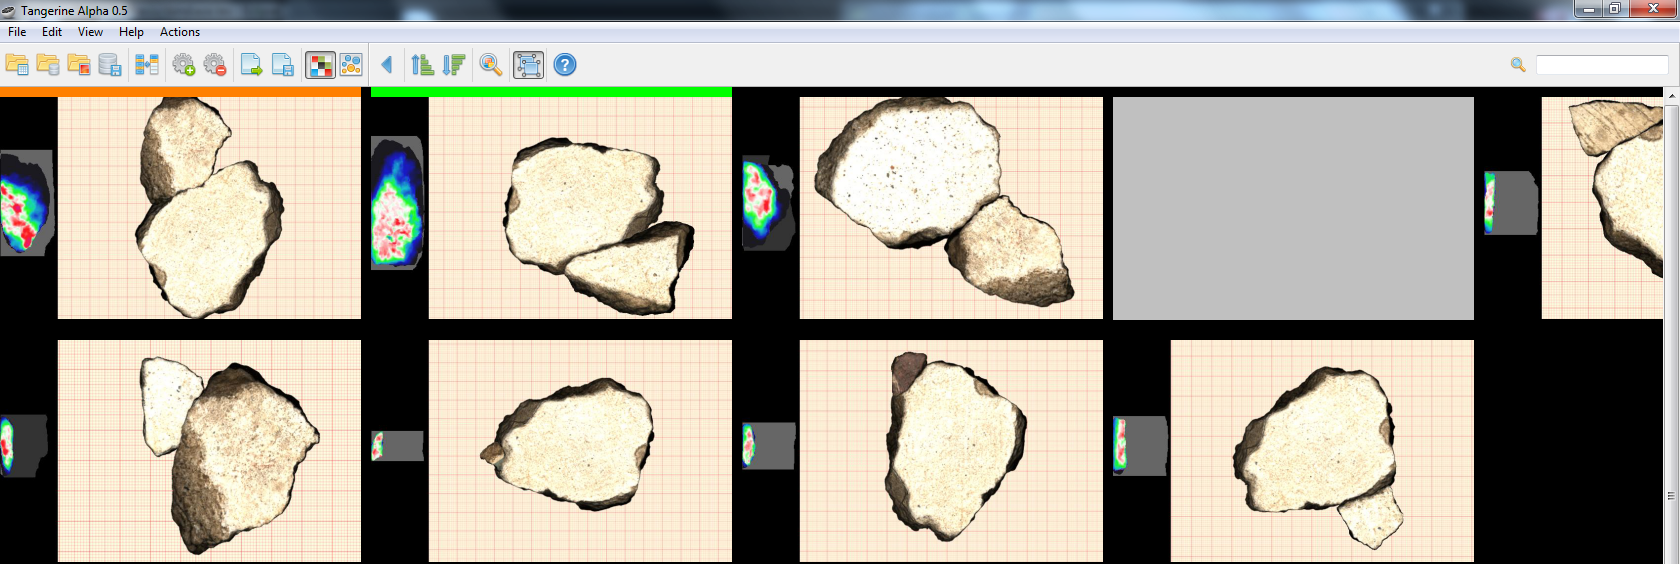
\includegraphics[width=1.0\columnwidth]{images/matchtileview-progconflict-01-reduced.png}
		\caption{Paren die niet conflicteren met elkaar}
		\label{fig:tileview-progconflict}
	\end{center}
\end{figure}

\emph{MatchTileView} kan niet enkel gebruikt worden om te bekijken, maar ook om attributen te veranderen. Men kan onder andere commentaren toevoegen en validaties veranderen. Aanduiden dat bepaalde paren duplicaten zijn gaat ook, hoewel het gemakkelijker is dit door een algoritme te laten bepalen.\\

Als laatste is er kopieerfunctionaliteit, met de gebruikelijke sneltoetsen of het rechterklikmenu kunnen paren naar Griphos overgezet worden om ze in meer detail te bekijken.

\section{DetailView}
\label{sec:detailview}

\emph{DetailView} is een hulpmodule die door andere modules gebruikt wordt om weer te geven wat er kan bij elkaar gepuzzeld worden. Dit is gelijkaardig aan het tafelblad van Griphos, met het verschil dat men met \emph{DetailView} vrij kan navigeren in een 3D-wereld. Hun opzet is verschillend: met Griphos kan manueel gepuzzeld worden, terwijl \emph{DetailView} dient om automatische reconstructies te beoordelen. Dubbelklikken op alle voorstellen in figuur~\ref{fig:tileview-progconflict} zal deze aan elkaar zetten en weergeven in \emph{DetailView}. Het resultaat is figuur~\ref{fig:detailfull}.\\

\begin{figure}[ht]
	\begin{center}
		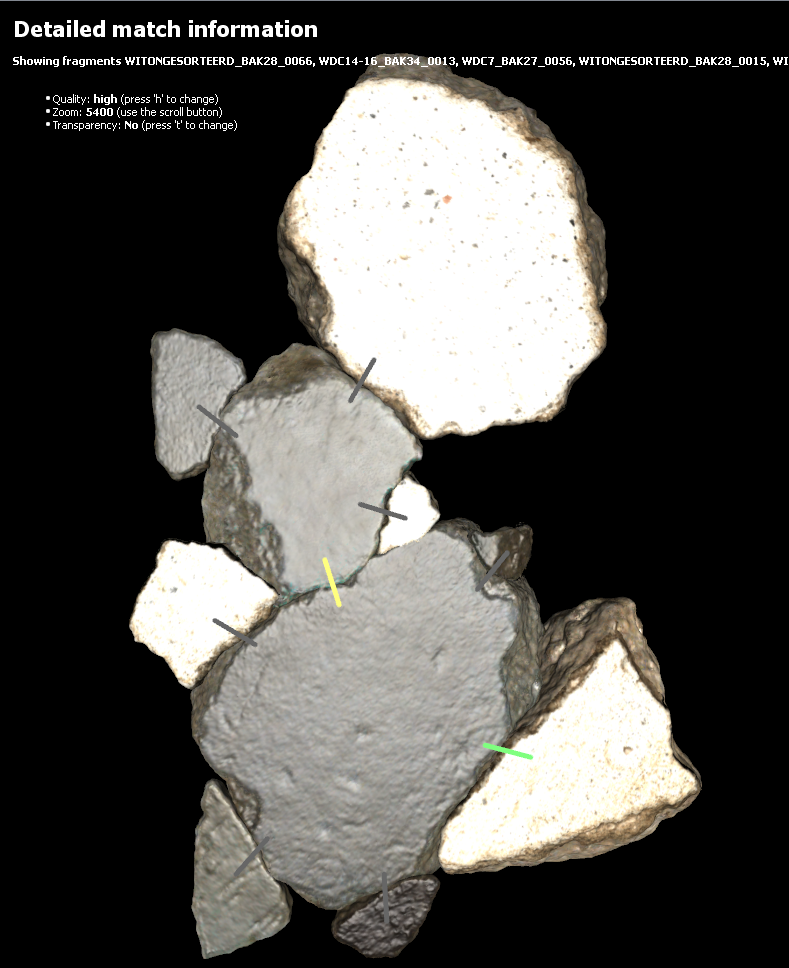
\includegraphics[width=1.0\columnwidth]{images/detailview-interesting-thin.png}
		\caption{\emph{DetailView}: De paren van figuur~\ref{fig:tileview-progconflict} aan elkaar gemaakt in 3D}
		\label{fig:detailfull}
	\end{center}
\end{figure}

\FloatBarrier

\begin{figure}[!hbt]
  \centering
  %\subfloat[De cluster]{\label{fig:detailfull}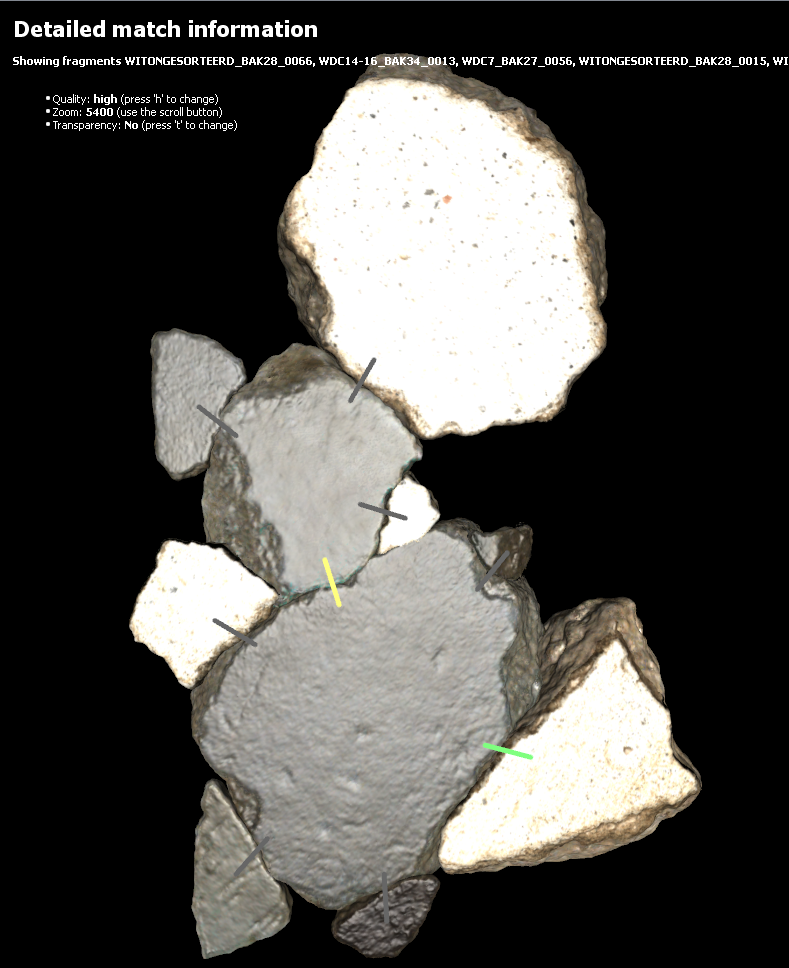
\includegraphics[width=0.33\textwidth]{images/detailview-interesting-thin.png}}                
  \subfloat[Een betere kijk op het interessante stuk]{\label{fig:detailzoom}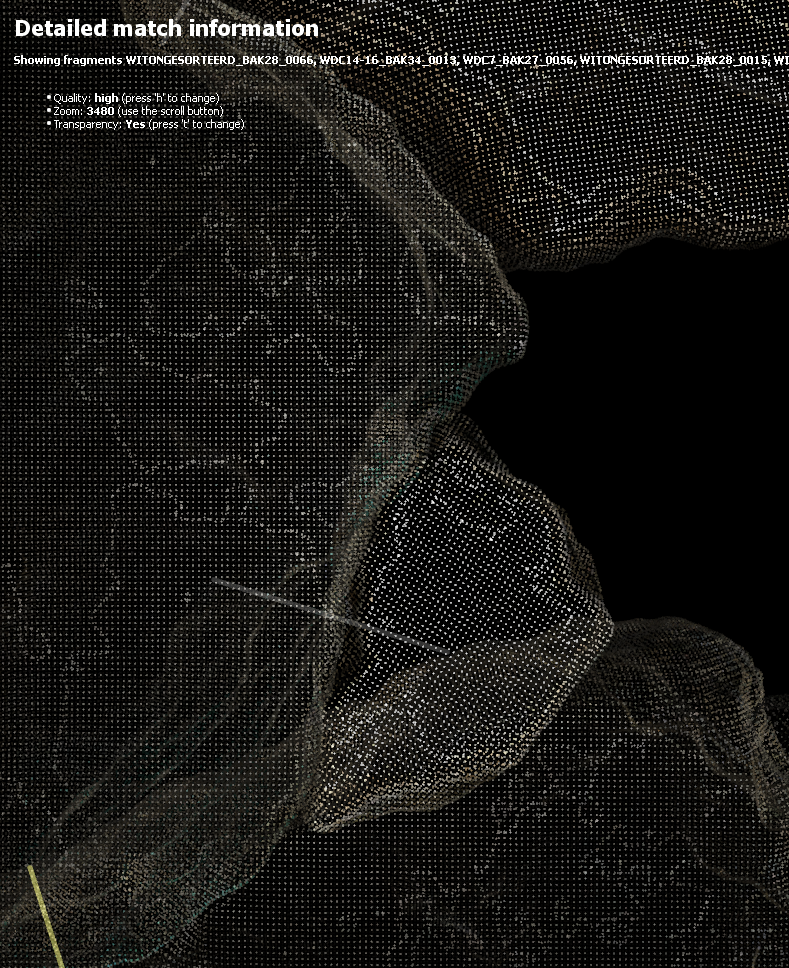
\includegraphics[width=0.47\textwidth]{images/detailview-interesting-thin-zoom.png}}
  \subfloat[De achterkant van het interessante stuk]{\label{fig:detailreverse}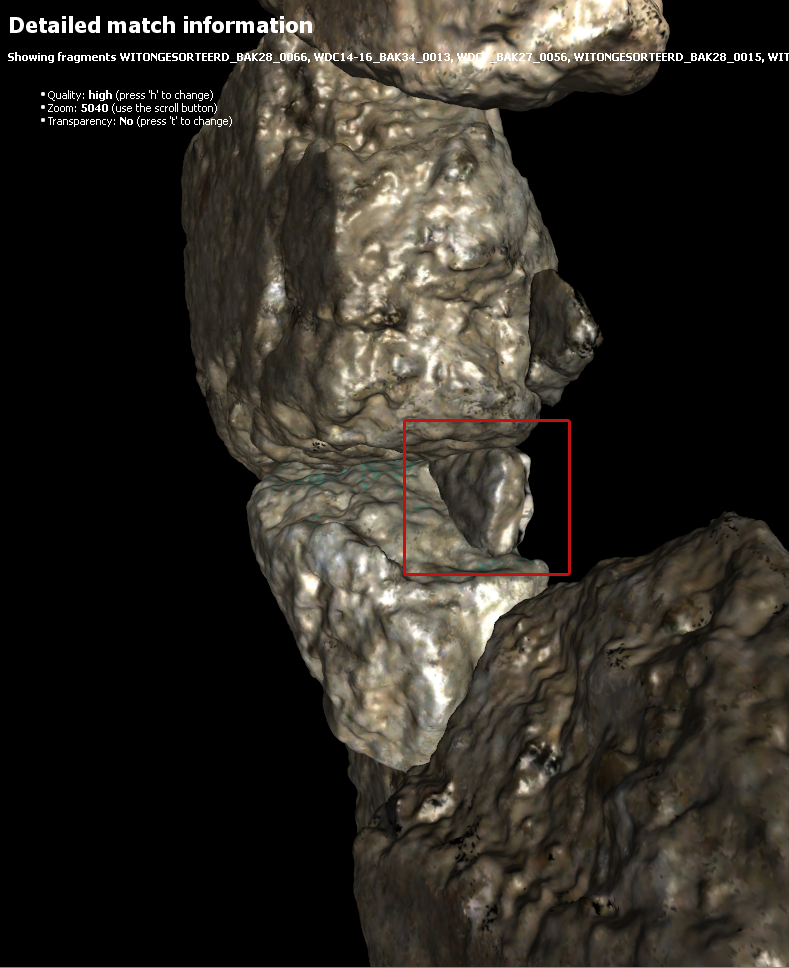
\includegraphics[width=0.47\textwidth]{images/detailview-interesting-thin-zoom-reverse-2.png}}
  \caption{\emph{DetailView} kan gebruikt worden om paren vanuit verschillende standpunten te bekijken}
  \label{fig:detail1}
\end{figure}

Figuur~\ref{fig:detailfull} is informatiever dan het dambordpatroon van \emph{MatchTileView} omdat het nuttige contextinformatie geeft. Het komt vaak voor dat door erosie een voorstel plausibel lijkt maar toch verkeerd is, maar het is veel minder waarschijnlijk dat drie fragmenten plausibel in elkaar passen en verkeerd zijn. Het kleine witte fragment dat geklemd zit tussen de twee grote grijze brokken is hier een voorbeeld van. Merk op dat de kleur van de fragmenten in dit specifieke voorbeeld niet zo relevant is\footnote{door vari\"erende brokstukkwaliteit en scancondities kunnen zelfs in een correct paar grote kleurverschillen optreden}, dit valt ook te merken in het grote kleurverschil bij het reeds goedgekeurde paar.\\

In eerste aanleg lijkt het er op dat een voorheen ongekende connectie is ontdekt, maar een dichtere inspectie toont een paar problemen. Figuur~\ref{fig:detailzoom} toont het geklemde fragment van dichterbij en geeft de geometrie weer als een puntenwolk, waardoor intersecties zichtbaar worden. Spijtig genoeg lijkt het erop dat een aanzienlijk volume van het geklemde fragment in het onderste grijze brokstuk zit\footnote{Dit is minder duidelijk op een kleine afbeelding maar goed te zien op een computerscherm, zeker als er tussen weergaven gewisseld wordt.}. De grafische voorstelling roteren onthult dat het geklemde fragment ook veel dunner is dan de rest, wat weer een aanwijzing is dat het misschien geen goed paar is. Desalniettemin zou dit best eens nagekeken worden met de echte brokstukken.

\section{GraphView}
Pure grafische plugins kunnen vertrouwen op andere plugins voor data-selectie: Om de werkbaarheid van dit systeem uit te testen werd een voorbeeldmodule ontwikkeld die alle huidige paren op een graaf plaatst en hier een ontwarringsalgoritme op toepast met behulp van de GraphViz bibliotheek. Deze voorstelling geeft een globaler beeld van de paren die aan de geldende criteria van het model voldoen.\\

Een gebruiksscenario is bijvoorbeeld om in \emph{MatchTileView} alle paren op te vragen die \emph{correct} of \emph{misschien correct} zijn, en daarna over te schakelen naar \emph{GraphView}. Dit werd gedaan op een database van 50000 paren, de criteria lieten er 245 over. Figuur~\ref{fig:graphyesmaybe} is het resultaat.\\

\begin{figure}[ht]
	\begin{center}
		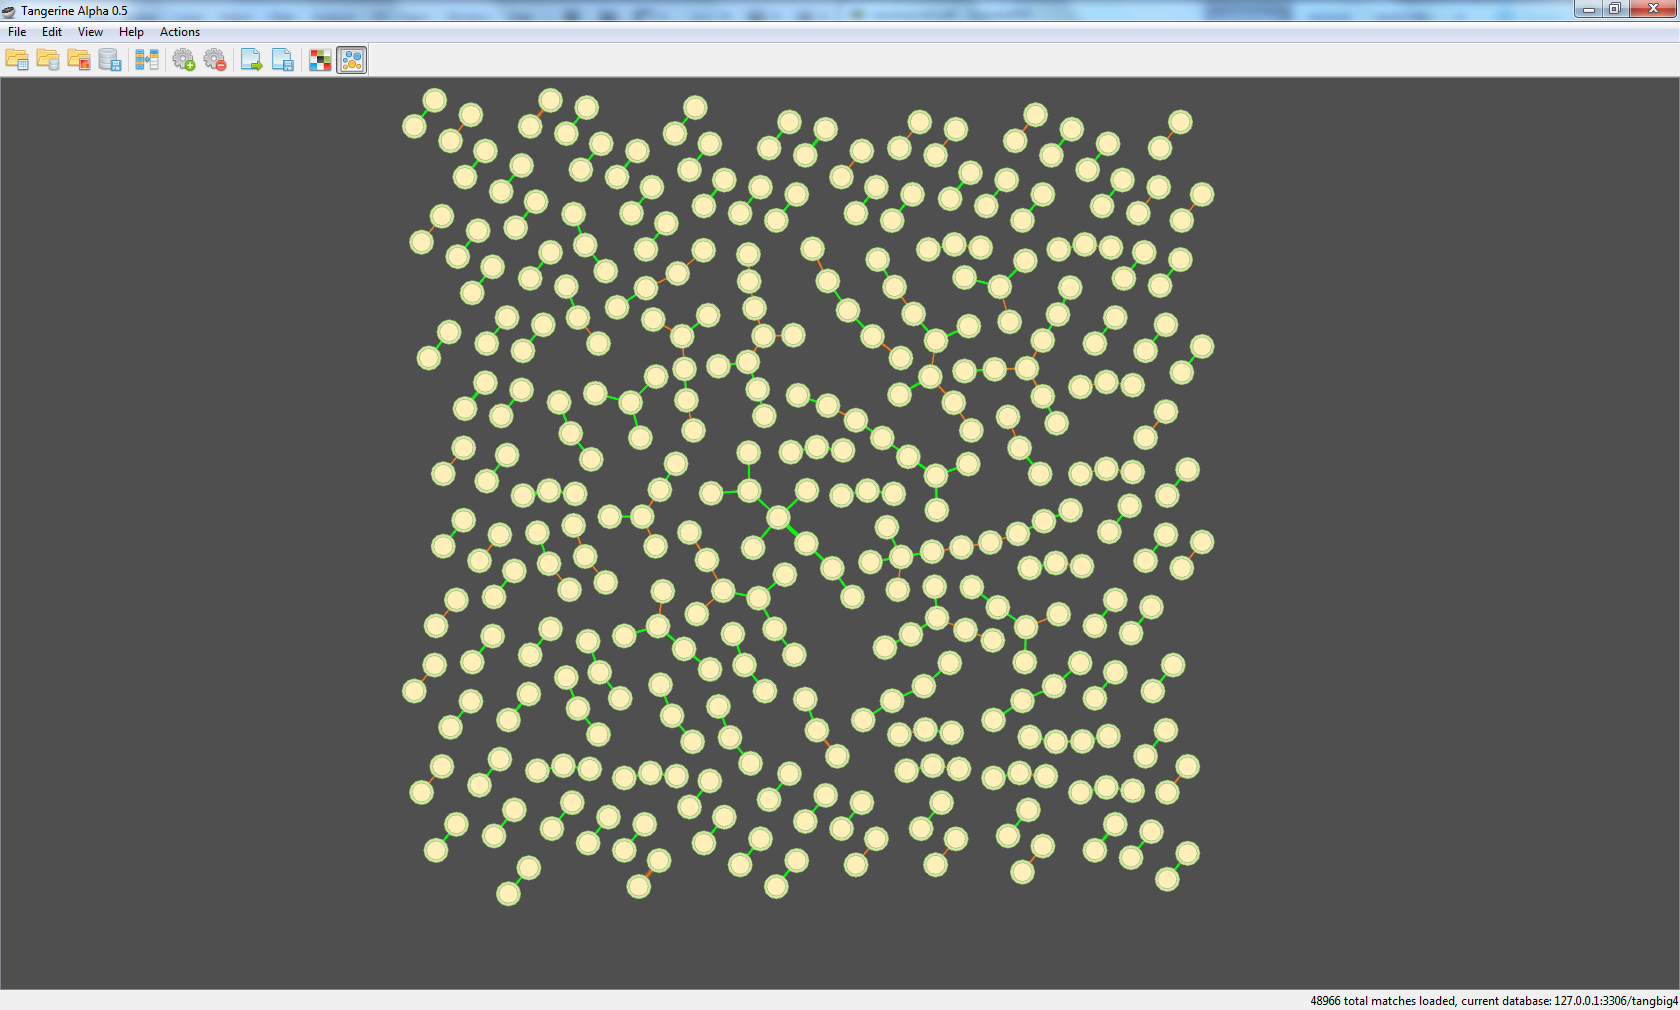
\includegraphics[width=1.0\columnwidth]{images/nodeview-yesmaybe.png}
		\caption{\emph{GraphView}: alle \emph{correcte} en \emph{misschien correcte} paren als een graaf voorgesteld}
		\label{fig:graphyesmaybe}
	\end{center}
\end{figure}

Hoe meer fragmenten er in een ketting aan elkaar kunnen gemaakt worden, hoe meer naar het midden ze worden gezet door het ontwarringsalgoritme. Nu de kettingen gemakkelijk zichtbaar zijn kunnen ze ook gevisualiseerd worden in 3D zoals in figuren~\ref{fig:graphchain1} en~\ref{fig:graphchain2}. Het valt op dat uit beide figuren gemakkelijk af te leiden valt welke \emph{misschien correcte} paren zeker niet correct zijn door naar de volumeoverlappingen te kijken (in~\ref{fig:graphchain1} zitten er zelfs een paar fragmenten volledig in een ander fragment).

\begin{figure}[ht]
	\begin{center}
		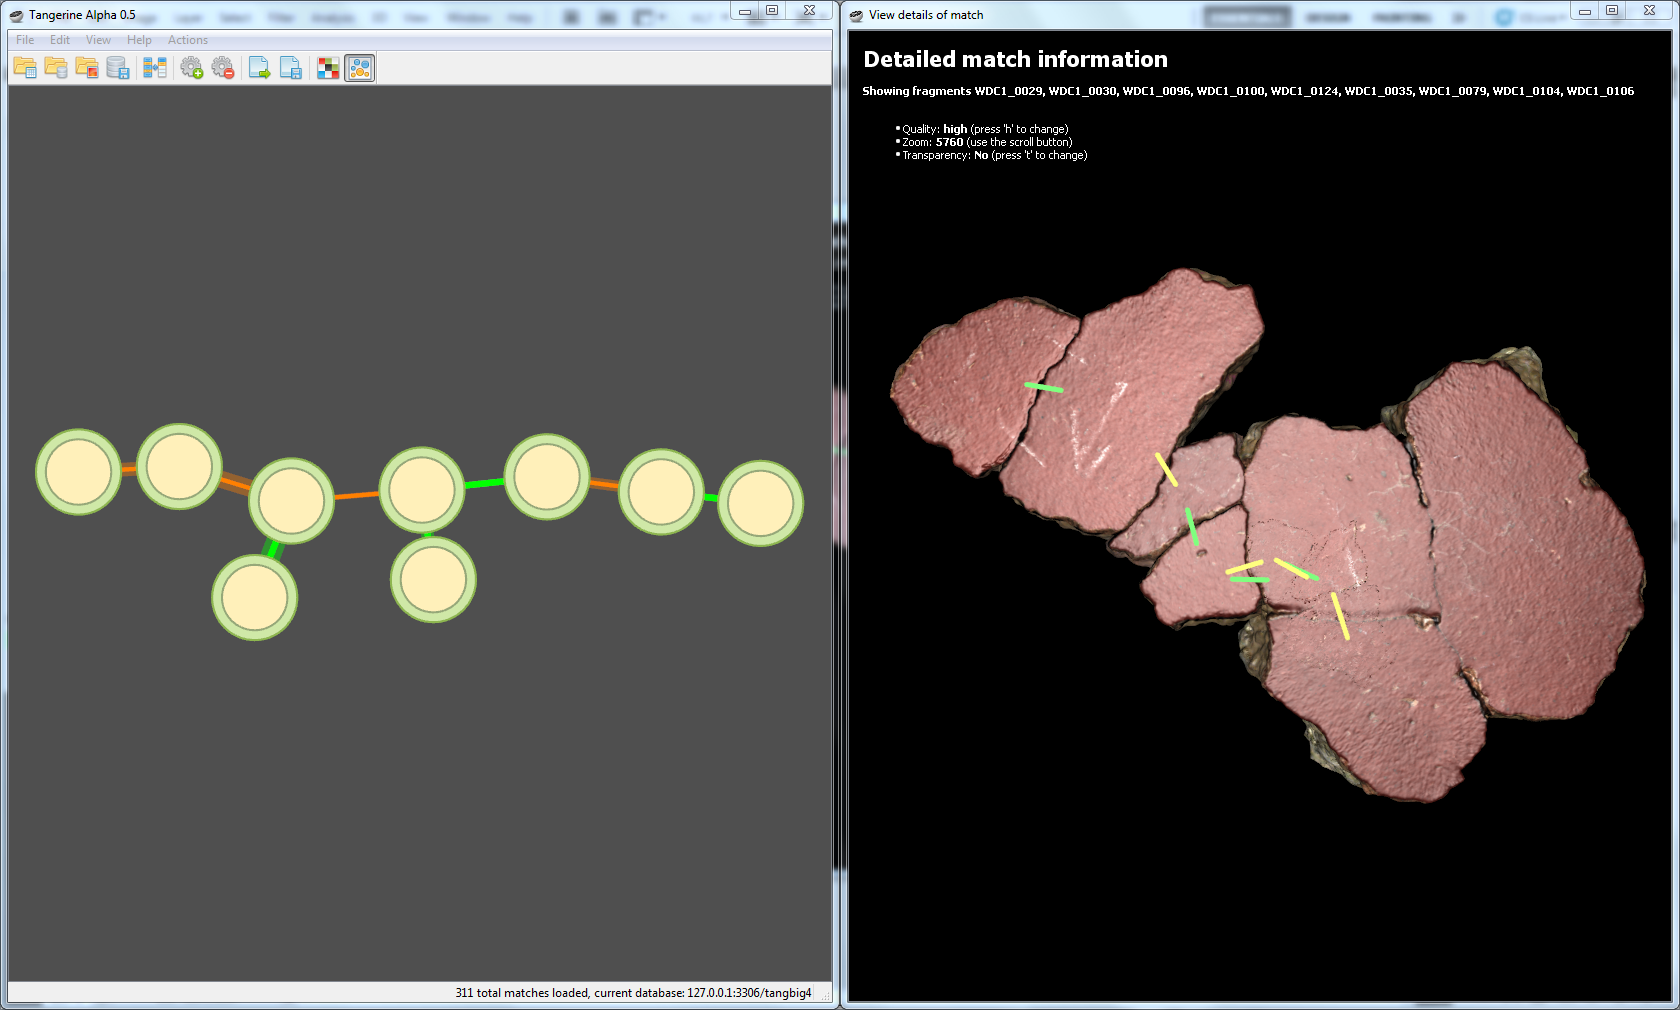
\includegraphics[width=1.0\columnwidth]{images/detailview-chain-02-rawcut.png}
		\caption{\emph{GraphView}: een ketting voorstellen in 3D}
		\label{fig:graphchain1}
	\end{center}
\end{figure}

\begin{figure}[ht]
	\begin{center}
		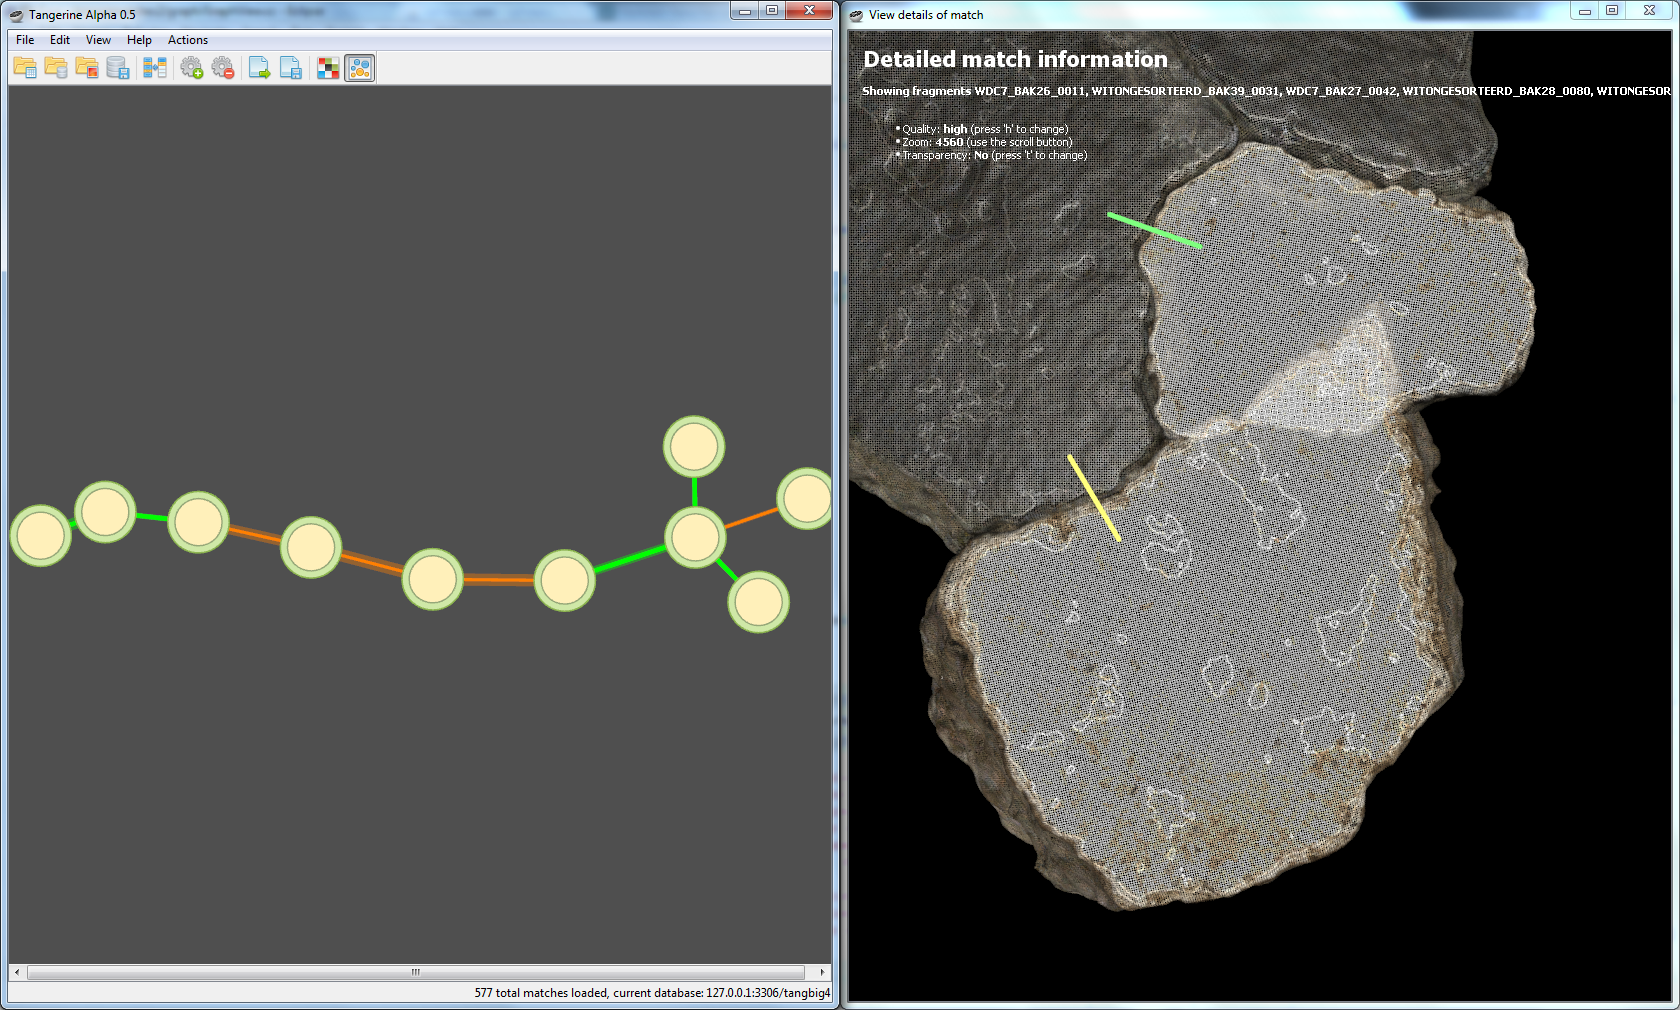
\includegraphics[width=1.0\columnwidth]{images/detailview-chain-10-rawcut.png}
		\caption{\emph{GraphView}: een andere ketting voorstellen in 3D}
		\label{fig:graphchain2}
	\end{center}
\end{figure}
%\chapter{Tests \& Vergelijkingen}
\label{hoofdstuk:tests}
Een goede manier om te weten te komen of het project zoals dit nut heeft gehad is om tests uit te voeren. Er zal worden vergeleken tussen de reeds bestaande oplossingen voor het classificeren van fragmentparen en de nieuwe applicatie waar mogelijk. In sommige gevallen zijn er nieuwe zaken toegevoegd die vroeger op geen of slechts manuele wijze mogelijk waren, hier zal worden vergeleken met (evt. fictieve) alternatieve implementaties. Voor het geval er helemaal geen vergelijking tussen alternatieven mogelijk is, zal een zo goed mogelijke maatstaf bedacht worden zodat er toch een beeld ontstaat van hoe de applicatie het doet.

\section{Use cases}
Elke gebruiker wenst met een applicatie een bepaald doel te bereiken, in dit geval is dat het classificeren van fragmentparen. Hiervoor zullen de mogelijkheden die het programma aanbiedt hopelijk zowel voldoende als gemakkelijk in gebruik zijn.

\subsection{Vind uit bak ONGESORTEERD het paar dat het meeste ruimte inneemt}
\subsection{Vind alle mogelijke paren die conflicteren met een waarschijnlijk paar}
\subsection{Vind alle mogelijke paren die grenzen aan het geselecteerde paar maar niet conflicteren ermee}
\subsection{Voeg een andere database bij de huidige, prefereer de veranderingen van de andere als er conflicten zijn}
\subsection{Gebruik conflict detectie \& 3D voorstelling om correcte paren te identificeren}
\subsection{Duid aan dat een verzameling mogelijke paren eigenlijk hetzelfde paar zijn (duplicaten)}
\subsection{Bekijk alle duplicaten van een paar}
\subsection{Vind alle paren die geclassificeerd staan als 'misschien'/'maybe', schrijf bij een paar je mening ('comment')}
\subsection{Exporteer een database naar een leesbaar formaat (XML)}
\subsection{Importeer een database van een leesbaar formaat (XML)}
\subsection{Kopi�er een aantal paren naar Griphos}
\subsection{Selecteer een aantal paren om te groeperen en in 3D weer te geven}

\subsection{Vindt wat je weet zijn: gebruik de zoek- en sorteerfuncties om snel een gewenst deel van de verzameling paren te zien}
\subsection{Vindt wat je niet weet zijn: gebruik de zoek- en sorteerfuncties om snel veelbelovende paren te vinden}
\subsection{Werken op een externe database (gebruiksgemak)}
\subsection{Databases samenstellen: conflicten oplossen}

\section{Snelheid (objectieve tests)}
\subsection{Opstartsnelheid}

\subsection{Inladen van fragmenten}
Meet het inladen van fragmenten, verschil tussen browsematches en tangerine (intern en extern)

\subsection{Navigeren tussen schermen}
Meet het navigeren tussen schermen, sorteren, filteren

\subsubsection{Teruggaan naar eerder schermen}
Door een caching mechanisme...

\section{Gebruiksgemak (subjectieve tests)}
Subjectieve waardeschattingen van gebruikers

\subsection{Intuitiviteit}
Het doelpubliek van de applicatie bestaat in de nabije toekomst uit archeologen en eventueel later uit amateurs die helpen met de classificatie. Qua gebruikersprofiel passen archeologen in het plaatje van een gebruiker met veel domeinkennis (classificeren), maar weinig kennis of ervaring met het gebruik van geavanceerde computerapplicaties. Anders gezegd: de gebruikers weten wat ze willen en moeten doen, maar niet noodzakelijk hoe ze het moeten doen in de applicatie.\\

Voor elk programma kan training voorzien worden zodat er uiteindelijk optimaal gebruik van kan gemaakt worden, maar het doel is om deze training tot een minimum te beperken. Dit houdt in dat de functies ontdekbaar\\

Informatie-popups (eenmalig/meermalig)

\subsection{Responsiviteit}
// MOVED NAAR DOELEN.TEX
Voor het dagdagelijkse gebruik van een applicatie is het van groot belang dat de gebruiker het niet hinderlijk vindt om ermee te werken. In enkele werken over gebruikersinterface ontwerp [aan elkaar?] [citatie] wordt erop gewezen dat de snelheid waarmee een applicatie reageert een sleutelfactor is voor het gebruiksgemak. Een algemene vaststelling: de tijd die een operatie mag innemen is omgekeerd evenredig met de frequentie waarmee deze operatie moet uitgevoerd worden. Deze regel in acht nemend is het duidelijk dat bijvoorbeeld het inladen van een scherm, het veranderen van een attribuut, het filteren en sorteren en dergelijke meer acties zijn die met de grootst mogelijke snelheid moeten worden uitgevoerd. \\

Voor al deze operaties is sinds het eerste ontwerp van de applicatie rekening gehouden met de implicaties van elke beslissing op de snelheid. Hierdoor is de snelheid van de applicatie op elke vlak verbeterd tegenover zijn voorgangers, soms op dramatische wijze. Om dit objectief vast te stellen zijn er een paar tests uitgevoerd:
\chapter{Toekomstig werk}
\label{toekomst}

Met dit project is ook een verdere stap gezet naar mobiele toepassingen. Het data-luik staat bijvoorbeeld toe om applicaties voor tablets te schrijven die beroep kunnen doen op een externe database om een groot deel van het zware werk over te nemen. Deze soort programma's kunnen het manueel verifi\"eren van paren sneller en aangenamer maken. De huidige werkwijze is als volgt: nadat er een resem waarschijnlijke paren zijn ge\"identificeerd, kan men de kisten met fragmenten uit de opslagruimte halen en nakijken welke er \'echt passen. Gezien de grote hoeveelheid brokstukken is het niet mogelijk om ze allemaal bij de hand te houden. Daardoor duurt het altijd even voor de gewenste fragmenten gevonden worden. In het slechtste geval wordt er gewerkt op een (krachtige) desktop. Hierdoor is het nodig is om ofwel de namen en locaties van de fragmenten te onthouden, of een heleboel afbeeldingen af te drukken. Na het fysisch testen van de fragmenten moet men dan terug naar de desktop om de bevindingen in te geven. Gelukkig behoort een laptop ook tot de mogelijkheden hoewel applicaties als Browsematches en Griphos niet bepaald licht zijn. Het performantieprobleem wordt natuurlijk reeds een deel verholpen door het invoegen van een externe database. Ook kan men nu gemakkelijker met meerdere mensen en laptops tegelijkertijd werken aan de validaties wegens de automatische synchronisatie. Een stap verder zou zijn om een tablet te gebruiken. Er zijn reeds in het verleden experimenten geweest binnen het thera project om aanraakgevoelige omgevingen te maken en de hoop is dat tesamen met de resultaten van deze thesis er in de toekomst iets concreets van gemaakt kan worden.

Het versturen van afbeeldingen over het netwerk! (hoe dit efficient te doen? niet opnieuw uitvinden van het wiel, gebruik een goede codec)
\chapter{Besluit}
\label{besluit}

Dit thesisproject heeft een lange weg afgelegd, waarbij er vaak geen duidelijk doel te bespeuren was, of beter gezegd geen concreet doel (vaag vaag).

Net zoals een gebroken fresco in feite een puzzel is, kan men het thera project zien als de som van vele delen die in elkaar passen. Dit thesisproject is bedoeld als een stuk dat een ander perspectief biedt op het geheel en het in staat moet stellen om meer en sneller resultaten te boeken. Het complementeert de bestaande aanpakken en zorgt ervoor dat de resultaten van de automatische paarherkenning nog nuttiger gebruikt kunnen worden. Omdat het validatiewerk noodzakelijk door mensen moet gebeuren, kan dit niet zonder meer opnieuw door een algoritme gedaan worden indien er iets misloopt. De in dit thesisproject geproduceerde componenten proberen er onder andere voor te zorgen dat dit zo min mogelijk voorkomt.\\

Op het vlak van ontginning van nuttige informatie met nieuwe visualisaties en nieuwe manieren om de juiste patronen te ontdekken zijn er natuurlijk nog steeds vele opportuniteiten. Want --- zoals opgemerkt in een recente paper over het thera project [citatie siggraph submission 2011] --- het vinden van de juiste paren is zoals zoeken naar een naald in een hooiberg. Met elke nieuwe toevoeging aan de mogelijkheden van het platform is er de kans dat deze een manier is om de hooiberg te verkleinen, door te lichten met X-stralen of gewoonweg op een grote krachtige magneet in een windtunnel te plaatsen. Naar deze laatste methode is iedereen natuurlijk op zoek. Tot dan is het zeker belangrijk dat men gemakkelijk kan experimenteren alsook bijhouden en opvragen welk deel van de berg reeds doorkamt is, waar de gevonden naaldrijke aders zitten en wat hun eigenschappen zijn. Wie weet zijn de naalden immers niet van metaal\ldots

% Indien er bijlagen zijn:
\appendixpage*  
\appendix
\chapter{Extra afbeeldingen \& schema's}
\label{app:A}

\section{Omzetting SQL naar NoSQL}
\begin{center}
\hvFloat[
%floatPos=h,
nonFloat=true,
capWidth=1,%
capPos=b,%
rotAngle=0,%
objectPos=c%
]{figure}{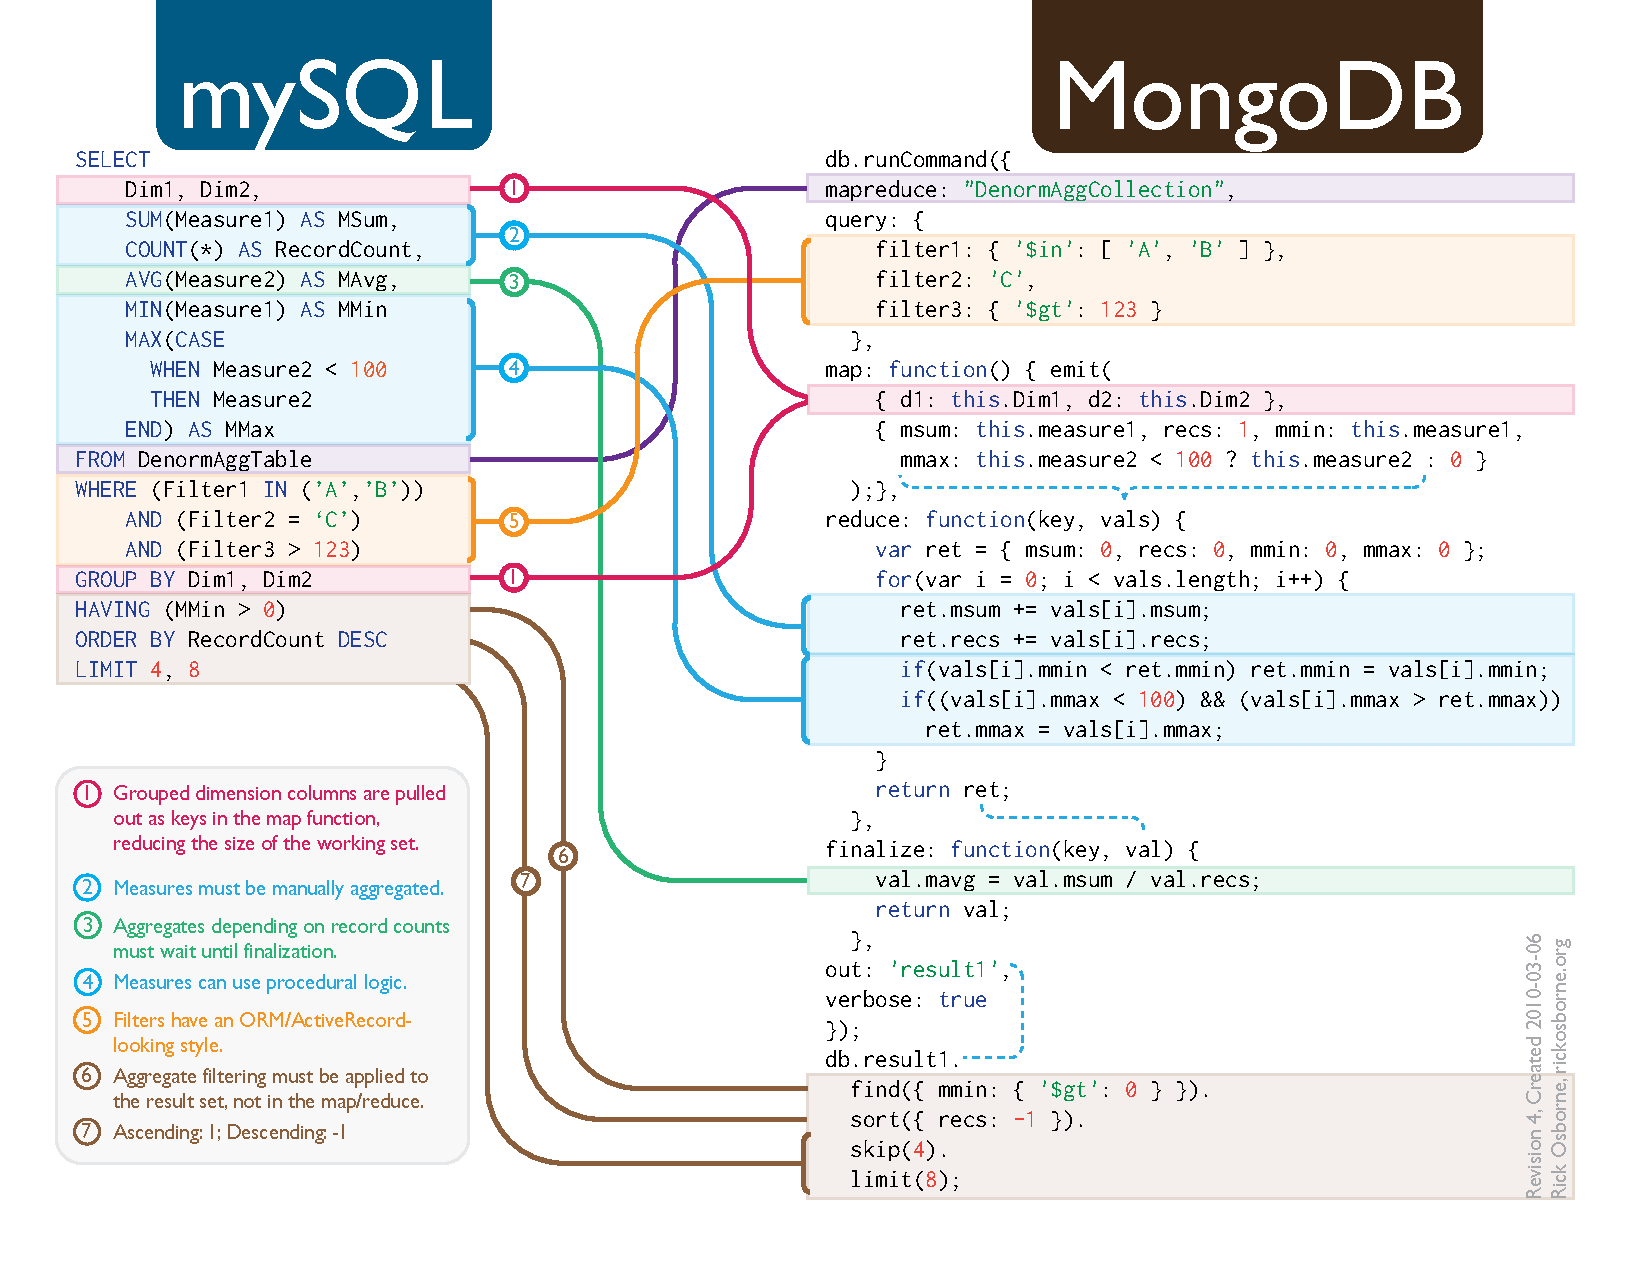
\includegraphics[width=0.7\textheight]{images/SQL-to-MongoDB.pdf}}{Sommige NoSQL systemen --- zoals MongoDB --- beschikken zoals te zien valt in deze afbeelding over dezelfde analytische kracht als een SQL database. De performantiekarakteristieken zijn echter verschillend. Afbeelding gebruikt met toestemming~\cite{sqlnosql}}{fig:sqlmongo}
\end{center}

%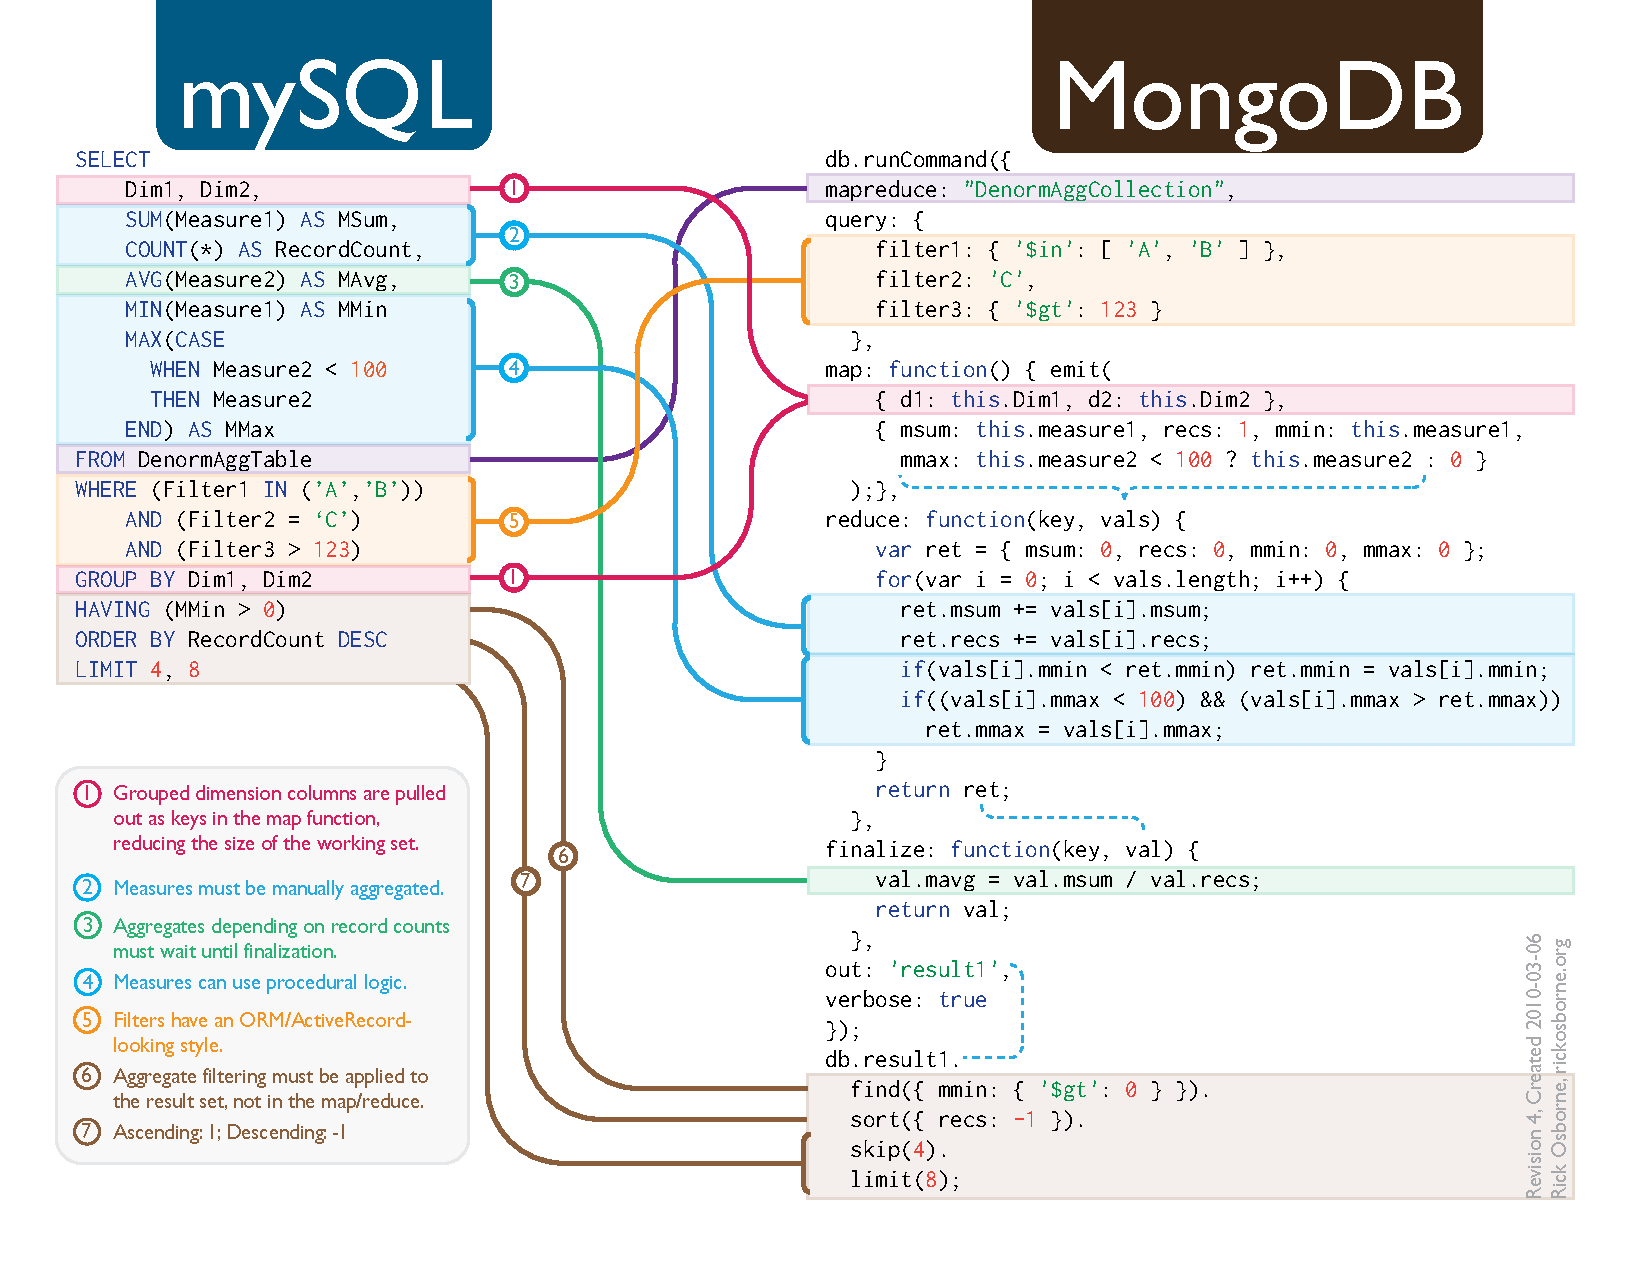
\includegraphics[width=0.8\textheight]{images/SQL-to-MongoDB.pdf}
%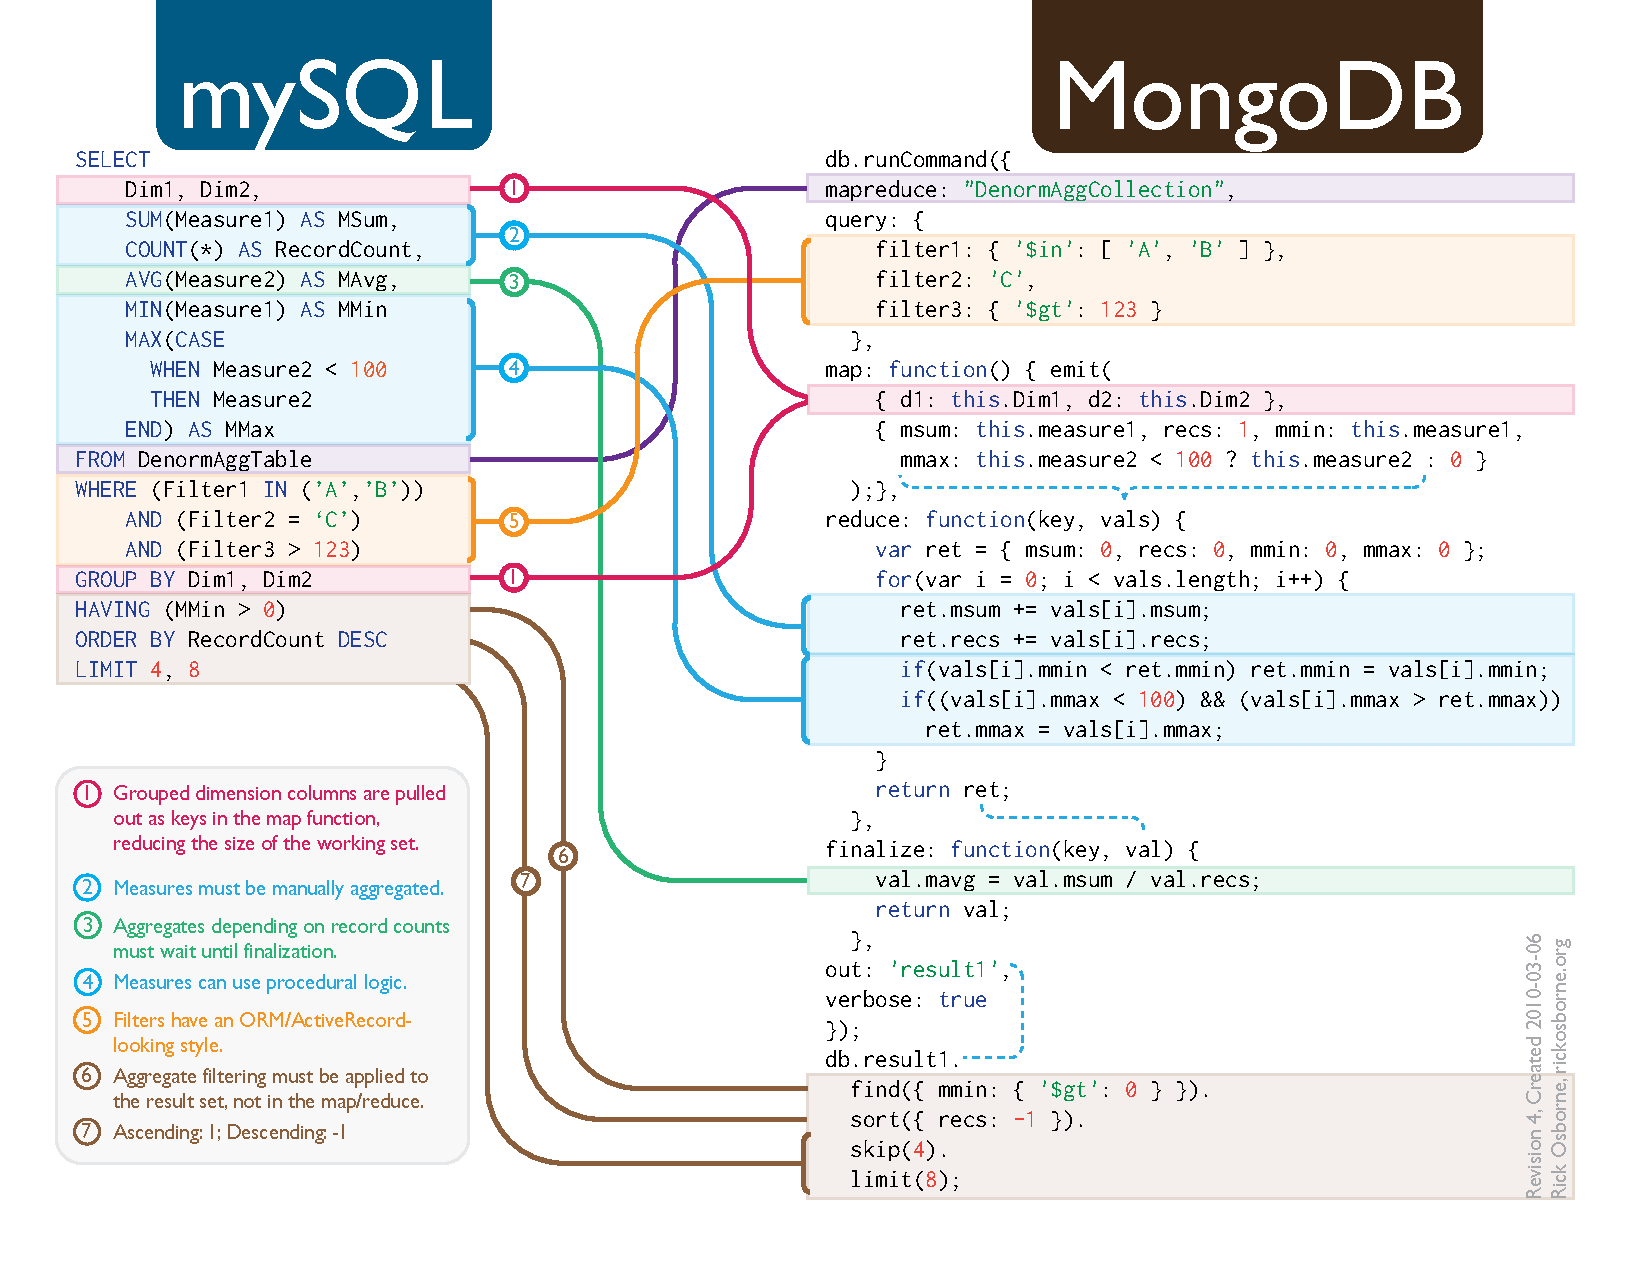
\includepdf{images/SQL-to-MongoDB.pdf}

\section{Componenten}
\hvFloat[
%floatPos=h,
nonFloat=true,
capWidth=1,%
capPos=b,%
rotAngle=90,%
objectPos=c%
]{figure}{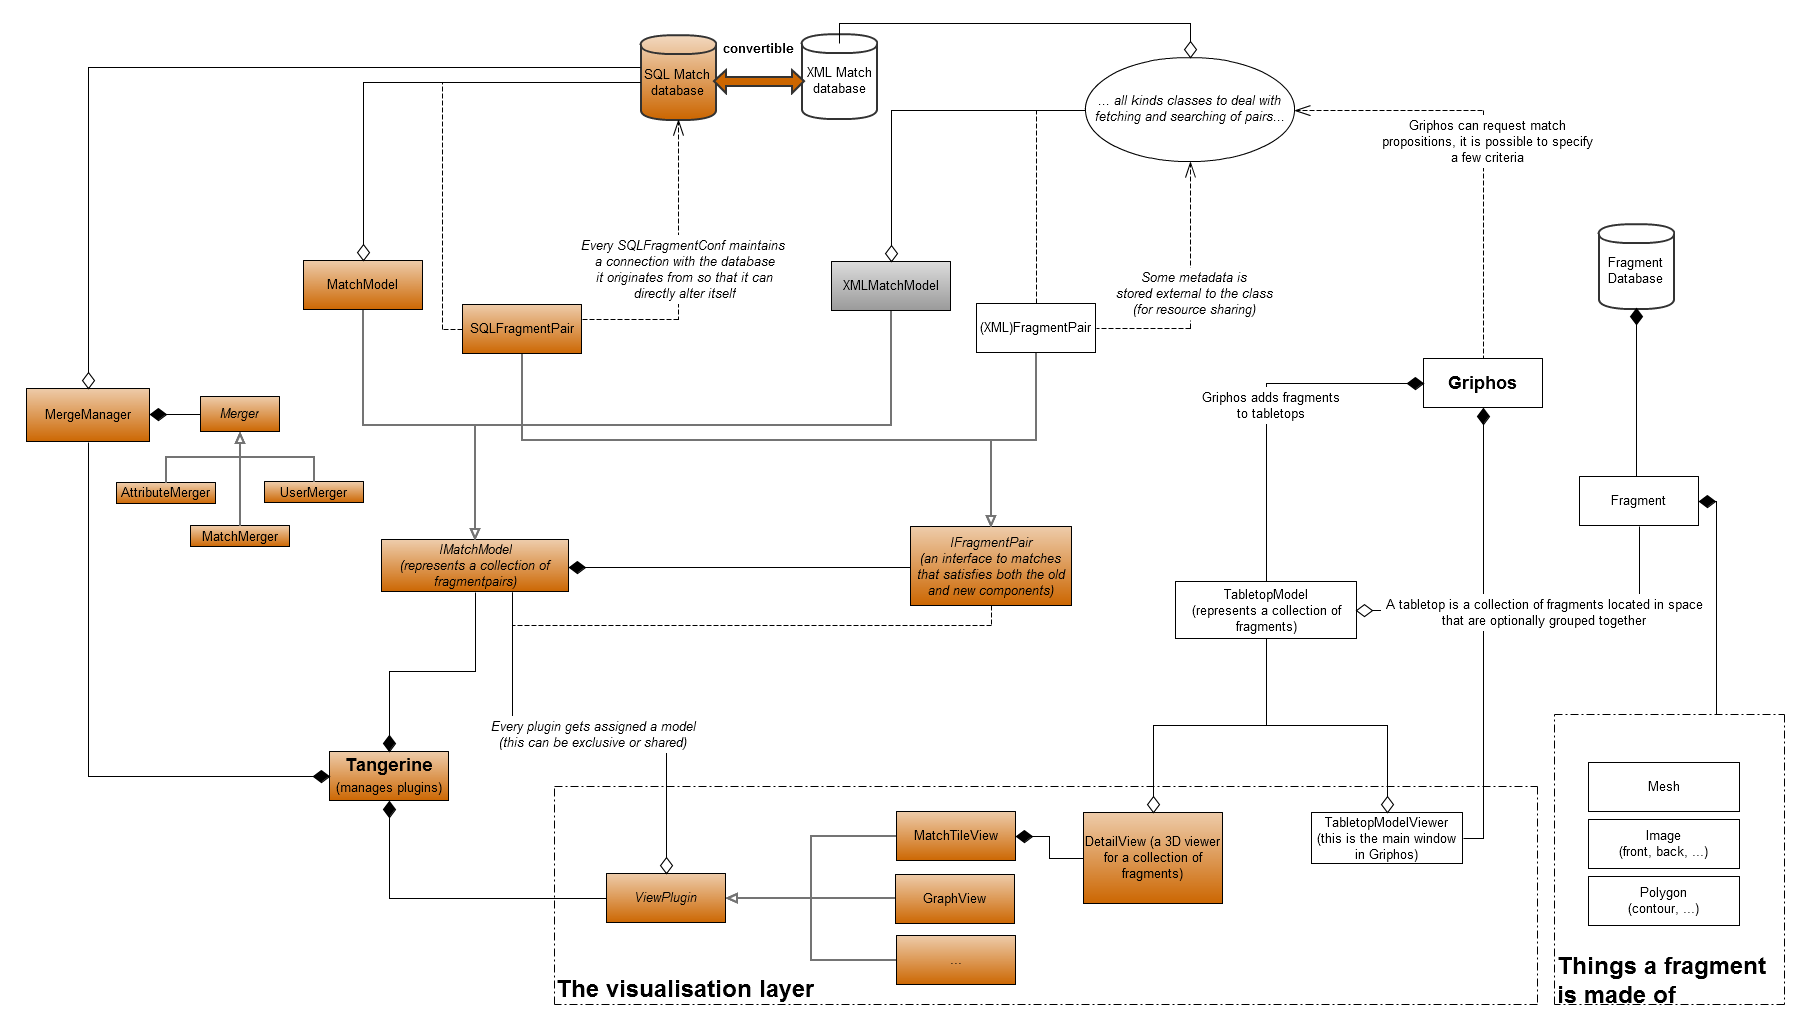
\includegraphics[width=0.95\textheight]{images/Bigtang.png}}{Een ruw overzicht van de componenten in het project en hoe het interageert met het reeds bestaande systeem.}{fig:tangbig}


\clearpage

\backmatter
%\bibliographystyle{abbrv}
\bibliographystyle{ieeetr}
\bibliography{referenties}

\end{document}
